\documentclass{thesis}
\newcommand{\normal}[2]{\mathcal{N}\left(\, {#1} \,,\,~{#2} \,\right)}
\newcommand{\multinormal}[4]{\mathcal{N}_{#1\times #2}\left(\, {#3} \,,\,~{#4} \,\right)}
\newcommand{\matrixnormal}[4]{\mathcal{MN}_{#1,#2}\left(\, {#3} \,,\,~{#4} \,\right)}

\newcommand{\vect}[1]{\boldsymbol{\mathbf{#1}}}
\newcommand{\mat}[1]{\boldsymbol{\mathbf{#1}}}

\newcommand{\tbm}[1]{$\mathbf{#1}$}
\newcommand{\tvect}[1]{$\boldsymbol{\mathbf{#1}}$}
\newcommand{\tmat}[1]{$\boldsymbol{\mathbf{#1}}$}

%\newcommand{\bm}[1]{\mathbf{#1}}
\newcommand{\paren}[1]{\left(#1\right)}

\newcommand{\texto}[1]{~~\text{#1}~~}

\newcommand{\til}[1]{\tilde{#1}}




\newcommand{\bfy}{\mathbf{y}}
\newcommand{\bfb}{\mathbf{b}}

\newcommand{\pinv}[1]{{#1}^{\dagger}}
\newcommand{\inv}[1]{{#1}^{-1}}
\newcommand{\trans}[1]{{#1}^\intercal}

\newcommand{\rmA}{\mathrm{A}}
\newcommand{\rmB}{\mathrm{B}}
\newcommand{\rmF}{\mathrm{F}}
\newcommand{\rmG}{\mathrm{G}}
\newcommand{\rmL}{\mathrm{L}}
\newcommand{\rmR}{\mathrm{R}}
\newcommand{\rmK}{\mathrm{K}}
\newcommand{\rmX}{\mathrm{X}}
\newcommand{\rmW}{\mathrm{W}}
\newcommand{\rmU}{\mathrm{U}}
\newcommand{\rmV}{\mathrm{V}}

\newcommand{\bfalpha}{\boldsymbol{\alpha}}
\newcommand{\bfbeta}{\boldsymbol{\beta}}


\newcommand{\calL}{\mathcal{L}}

\newcommand{\nullH}{\mathcal{H}_0}
\newcommand{\altH}{\mathcal{H}_1}
\makeglossaries 
%\setabbreviationstyle{long-short-sc}% glossaries-extra.sty
\loadglsentries{abbreviations.tex}

\addbibresource{references.bib}
\begin{document}
\glsenablehyper
\hyphenation{
cross=va-li-da-tion
high=di-men-sio-nal
low=di-men-sio-nal
ge-no-type=phe-no-type
SNP-phe-no-ty-pe
ge-nome=wide
Phe-no-type-Si-mu-la-tor
ma-trix=va-ri-ate
Hu-man-Om-ni-Ex-press=24v1=0
de-signs
spa-tially=re-solved
l'Aca-de-mie
maxi-mum=like-li-hood
Men-de-li-an
Seid-man
dias-tro-phic
Ca-nes-sa
Gau-det
Kon-tro-gianni=Kon-stan-to-pou-los,
na-tur-for-schen-den
Me-di-zi-nisch=che-mische
chain=ter-mi-na-ting
post=trans-la-tio-nal
}


\cleardoublepage
\titlehead{
    \parbox{1\textwidth}{\centering
   			\includegraphics[height=12mm]{Figures/logos.pdf}}%
    \vspace{12mm}}
\title{Genetic association of high-dimensional traits}
\subject{This dissertation is submitted for the degree of Doctor of Philosophy}
\author{Hannah Verena Meyer}
\date{September 2017}
\publishers{%
    %\vfill doesn’t work properly on title page due to excess glue
    \vspace{6\baselineskip}
  	University of Cambridge\\
  	Jesus College\\[0.2\baselineskip]
    European Bioinformatics Institute}

\lowertitleback{%
    \centering
    {\footnotesize The source code of the thesis is available at
        \url{https://github.com/HannahVMeyer/thesis}.}}


\maketitle


\cleardoublepage
This dissertation is the result of my own work and includes nothing which is the outcome of work done in collaboration except as declared in the Preface and specified in the text.

It is not substantially the same as any that I have submitted, or, is being concurrently submitted for a degree or diploma or other qualification at the University of Cambridge or any other University or similar institution except as declared in the Preface and specified in the text. I further state that no substantial part of my dissertation has already been submitted, or, is being concurrently submitted for any such degree, diploma or other qualification at the University of Cambridge or any other University or similar institution except as declared in the Preface and specified in the text. 

This dissertation does not exceed the limit of \num{60000} words as specified by the Biology Degree Committee.
\cleardoublepage

\tableofcontents
\addcontentsline{toc}{chapter}{\listfigurename}
\listoffigures
\cleardoublepage
\addcontentsline{toc}{chapter}{\listtablename}
\listoftables
\cleardoublepage
\addcontentsline{toc}{chapter}{List of Abbreviations}
\printglossary[type=\acronymtype, title={List of Abbreviations}]
\cleardoublepage
\clearpage
\chapter*{Summary}
\addcontentsline{toc}{chapter}{Summary}
\label{section:summary}

\begin{singlespace}
Over the past ten years, more than \num{4000} genome-wide association studies (GWAS) have helped to shed light on the genetic architecture of complex traits and diseases. In recent years, phenotyping of the samples has often gone beyond single traits and it has become common to record multi- to high-dimensional phenotypes for individuals. Whilst these rich datasets offer the potential to analyse complex trait structures and pleiotropic effects at a genome-wide level, novel analytic challenges arise. This thesis summarises my research into genetic associations for high-dimensional phenotype data.

First, I developed a novel and computationally efficient approach for multivariate analysis of high-dimensional phenotypes based on linear mixed models, combined with bootstrapping (LiMMBo). Both in simulation studies and on real data, I demonstrate the statistical validity of LiMMBo and that it can scale to hundreds of phenotypes. I show the gain in power of multivariate analyses for high-dimensional phenotypes compared to univariate approaches, and illustrate that LiMMBo allows for detecting pleiotropy in a large number of phenotypic traits.

Aside from their computational challenges in GWAS, the true dimensionality of very high-dimensional phenotypes is often unknown and lies hidden in high-dimensional space. Retaining maximum power for association studies of such phenotype data relies on using an appropriate phenotype representation. I systematically analysed twelve unsupervised dimensionality reduction methods based on their performance in finding a robust phenotype representation in simulated data of different structure and size. I propose a stability criteria for choosing low-dimensional phenotype representations and demonstrate that stable phenotypes can recover genetic associations.

Finally, I analysed genetic variants for associations to high-dimensional cardiac phenotypes based on MRI data from \num{1500} healthy individuals. I used an unsupervised approach to extract a low-dimensional representation of cardiac wall thickness and conducted a GWAS on this representation. In addition, I investigated genetic associations to a trabeculation phenotype generated from a supervised feature extraction approach on the cardiac MRI data.

In summary, this thesis highlights and overcomes some of the challenges in performing genetic association studies on high-dimensional phenotypes. It describes new approaches for phenotype processing, and genotype to phenotype mapping for high-dimensional datasets, as well as providing new insights in the genetic structure of cardiac morphology in humans.


\end{singlespace}


% Increasing sample sizes have allowed to extend the genotype to phenotype mapping from common to rare variants.
% far beyond standard methods that work in the regime of up to 30 phenotypes. 

\titleformat{\chapter}[display]
{\filleft\bfseries}
{\filleft\chapnumfont\textcolor{chapnumcol}{\thechapter}}
{-2ex}
{\huge}

\chapter{Introduction}
The field of quantitative genetics has come far since Fisher's initial studies on human growth traits in 1918. Although the concept of inheritance existed at this time, little was known about the molecule responsible. The discovery of the DNA structure in the 1950s and technical break-throughs in analysing its sequence in the following decades have allowed to investigate genetic variance on a detailed scale, moving from whole chromosomes and linkage studies to the analysis of DNA variation on a single-base pair level. 

The developments in genotyping and sequencing technologies in recent years have made large scale studies on genetic variation feasible. With the sinking costs of genotyping techniques, the number of samples has risen and studies investigating the effects of single DNA bases often comprise thousands of individuals, in particular in the field of human genetics.  Together with the increased number of samples, the number of phenotypes that are measured for each individual has grown from a few measurements to tens, hundreds or even thousands. The availability of these rich datasets provides great opportunities when studying the influence of genetic variation on phenotypic variance. However, it also poses technical challenges when analysing these datasets. 

In this thesis, I identified some of these challenges and propose new methods for the genetic analysis of high-dimensional datasets. These new methods are first explored on simulation studies and subsequently applied to real datasets. Specifically, I developed a new approach for the joint genetic association testing of a large number of phenotypic traits and applied this method to a publicly available dataset of yeast growth traits. I explored different dimensionality reduction methods for very high-dimensional datasets and propose a new measure to define the stability of the dimensionality reduction. Finally, I analysed human heart morphology data for genetic associations, applying the methods from the dimensionality reduction study on simulated data. In this introduction, I will first give a general overview of the history and methods in quantitative genetics, followed by the description of statistical models relevant for this thesis. In order to help with an understanding of the genetic association studies on the human heart morphology data, I also introduce basic concepts of cardiac structure and development and their underlying genetics. 

\section{From ancient ideas of inheritance to the birth of modern genetics}
The formulation of the concept of human inheritance --the passing on of traits from parents to offspring-- can already be found in works of Hippocrates and Aristotle. In addition to their theory of the inheritance of acquired traits, Hippocrates and Democritus also describe a possible mechanism of inheritance \citep{Zirkle1935}, a concept later formalised as \textquote{pangenesis} by the English naturalist Charles Darwin \parencite*{Darwin1868} and others such as the French Comte de Buffon \parencite*{Buffon1749} and Genevan naturalist Charles Bonnet \parencite*{Bonnet1779}. The theory of pangenesis -- which translates to whole (Greek: pan) origin (Greek: genesis) or birth (Greek: genos) -- describes how the entire parental organism participates in passing on traits to the offspring. In this developmental theory of heredity, all cells in an organism were believed to secrete small particles called gemmules, which circulate through the body to congregate in the gonads. While this theory was quickly refuted, Darwin became renowned for his ideas about trait variation and the link to inheritance. In his famous work \textit{On the Origin of Species} \parencite*{Darwin1859}, he postulates natural selection as the central concept of evolution, based on his observations of phenotypic variance in a population, differential fitness based on phenotype and the concept of heritability of this fitness \citep{Lewontin1970}. 
\\
\\
The milestones in genetics made since Darwin's work \textit{On the Origin of Species} as well as accompanying statistical models and techniques in molecular biology are depicted in \cref{fig:timeline-genetics}.

\begin{figure}[hbtp]
	\centering
	\includegraphics[trim = 0mm 0mm 0mm 0mm, clip, width=\textwidth]{Introduction/Figures/TimelineQuantGenetics.pdf}
	\caption[\textbf{Genetics over time. }]{\textbf{Genetics over time. } A. Statistical concepts and B. techniques in molecular biology crucial for the advances in genetics. C. The developments in genetics from its birth by Mendel's Laws of Inheritance to large databases cataloguing genetic variation of thousands of individuals. Whilst there are many independent studies in all three areas contributing to the successes in genetics that we observe today, I have attempted to depict all major events that lead to the specific field of human quantitative genetics in the GWAS era. The development of mathematical models is focused towards models used in this thesis. The legend below the timelines specifies the symbols of the organisms used in the respective studies. As references for each entry, the first author of the corresponding publication is shown. Discoveries where multiple authors are named indicate independent studies at the same time making the same discovery/developing techniques. } 
	 	\label{fig:timeline-genetics}
\end{figure}


\subsection{Mendelian Laws of Inheritance}
The Austrian friar Gregor Mendel was the first to systematically study the mechanisms of heritability. By cross-breeding different varieties of pea plants, he was able to follow the inheritance patterns of a number of visually-observable traits such as flower colour, seed shape and plant height. In 1866, he presented his observations in the paper \textit{Versuche über Pflanzenhybride} (experiments on plant hybridisation) where he proposes three general concepts of inheritance which later became known as the Mendelian Laws of Inheritance: i) the Law of Independent Segregation (every individual contains two alleles for each trait which segregate in germ cells leading to a random transmission of alleles to the offspring), ii) the Law of Independent Assortment (traits are inherited independently of each other) and iii) the Law of Dominance (recessive alleles will be masked by dominant alleles and the trait corresponding to the dominant allele will be observed) \citep{Mendel1866}. Although his work stayed widely unnoticed during his lifetime, his meticulous studies and documentation ensured his recognition as the father of genetics. In 1900, his work was independently rediscovered by the Dutch botanist Hugo de Vries \citep[translation into English]{deVries1900,Hannah1950} and --although contested by some based on their seeming lack in understanding of Mendel's work \citep{Keynes2008,Monaghan1986,Monaghan1987}-- the German botanist Carl Correns \citep[translation into English]{Correns1900,Piernick1950} and the Austrian agronomist Erich Tschermak \parencite*{Tschermak1900}. 

Around the same time, the British geneticist William Bateson set out to make Mendel's work accessible to the scientists not proficient in Mendel's native language German. He translated Mendel's original papers on the Laws of Inheritance \citep{Mendel1866} and cross-breeding studies in \textit{Hieracium} \citep{Mendel1869} into English and published them in \textit{Mendel's Principles of Heredity: a Defense} \citep{Bateson1902}. In \parencite*{Bateson1909}, Bateson published an extended version of his original book which allowed Mendel's work to become known in the greater scientific world \citep{Keynes2008}, more than 40 years after their original publication. In addition to this work, the book \textit{Recent Progress in the Study of Variation, Heredity, and Evolution} by his former student Robert H. Lock should be mentioned as the first English textbook embracing Mendel's ideas of inheritance \citep{Lock1906,Edwards2013}.

In addition to the rediscovery and translation of Mendel's ideas into English, two other branches of investigations contributed to the understanding of heredity and the identification of the molecular basis of the Laws of Inheritance from 1900 onward: biometrics and molecular biology. 

\subsection{Biometrics}
Inspired by Darwin's work on evolution, his half-cousin Francis Galton was interested in mathematically describing and analysing evolutionary concepts. In 1886, he published  \textit{Regression Towards Mediocrity in Hereditary} \textit{Stature}, offering a statistical approach towards understanding inheritance. Based on measurements of height in parents and their children, he observed that the \textquote{[t]he height-deviate of the offspring is, on the average, two-thirds of the height-deviate of its mid-parentage}. He achieved the quantification of the deviation from the mean by fitting straight lines to the observed heights and finding their slope, thereby developing the technique of linear regression analysis and introducing the concept of correlation \citep{Galton1886}. An extension of this work and descriptions of different statistical distributions and processes in heredity were published in his book \textit{Natural inheritance} \citep{Galton1889}. Karl Pearson formalised and extended Galton's statistical models for quantifying the effects of inheritance on trait variance by introducing the concept of p-values, the Chi-sqare test and \gls{pca} \citep{Pearson1900,Pearson1901}. The marine biologist Walter Weldon applied these statistical concepts to data he had collected on shrimps and crabs \citep{Weldon1890, Weldon1892}, demonstrating selection in natural populations. Together, Galton, Pearson and Weldon are known as the founders of biometrics, the science of applying statistical methods to the study of evolution on quantitative traits, or as Galton described it: \textquote{The primary object of Biometry is to afford material that shall be exact enough for the discovery of incipient changes in evolution which are too small to be otherwise apparent.} \citep[editorial]{Galton1901}. Despite the progress in understanding evolution in the light of statistical concepts, their direct study of heredity was impeded by their reluctance to acknowledge the validity of Mendelian genetics \citep{Bulmer2003}.

\subsection{Molecular basis of inheritance}
Advances in understanding the molecule responsible for inheritance were made by the Swiss physican and biologist Johannes Miescher and the German anatomist Walther Flemming.  \citet{Miescher1871} was the first to successfully isolate a substance he called \textit{nuclein} --later known as DNA-- from the nucleus . Flemming's experiments on salamander cells lead to the discovery of structures that could easily be stained by basophilic dies and he named them \textit{chromatin} --  \textquote{coloured material} (greek:khrōmat). He later found chromatin to be originating from the cell nucleus and did further studies into understanding cell division and mitosis \parencite*{Flemming1878}. Although both Miescher's and Flemming's methods and discoveries were crucial in the later identification of DNA as the carrier of inheritance, neither of them made the connection at the time. 
\\
With these advances in molecular and statistical techniques and the rediscovery of the Mendelian laws, the new discipline of genetic research attracted much attention. 

\section{The Laws of Inheritance on a cellular level}
The first two scientists proposing how Mendel's Laws could work on a cellular level were the German biologist Theodor Boveri and the American Walter Sutton. By experimentally introduced double-fertilisations of sea urchin eggs and subsequent observations of developmental processes in the resulting embryos, Boveri claimed \foreignquote{german}{dass eine bestimmte Kombination von Chromosomen zur normalen Entwicklung notwendig ist, und dieses bedeutet nichts anderes, als dass die einzelnen Chromosomen verschiedene Qualit\"{a}ten besitzen m\"{u}ssen.}  i.e. \textquote{that a specific combination of chromosomes is necessary for a normal development which in turn means that each chromosome must harbour different qualities} \citep{Boveri1902}. 

At the same time, Sutton described his observations in reduction division (later known as meiosis) and postulated that different chromosomes play different roles in development. Similar to Boveri, he came to the conclusion that \textquote{the phenomena of germ cell division and of heredity are seen to have the same essential features \textelp{}, with purity of units (chromosomes, characters) and the independent transmission of the same} \parencite*{Sutton1903}. Both studies demonstrated the link between the Mendelian Laws of Inheritance and chromosomes as its carrier and are the basis for the chromosome theory of inheritance, also known as Boveri-Sutton Chromosome theory. 

Around the same time, Bateson worked together with Edith Saunders and Reginald Punnett on experiments similar to Mendel's pea hybrids to understand the physiology of heredity. While they confirmed Mendel's original observations, they also discovered traits whose segregation did not follow the Law of Independent Assortment. Although they could not explain the mechanism of these observations, their results lead them to propose the concept of coupling or co-inheritance of traits \citep{Bateson1905}. The first suggestion that this coupling of traits might result from genes lying on the same chromosome came by \citet{Lock1906,Edwards2013}. 

With the progress in understanding Mendelian Laws on a cellular level came the establishment of terms describing certain entities and properties that are still in use today. In addition to his scientific contributions and his translation of Mendel's works into English, Bateson became known for coining key terms in the field of genetics, even the term genetics itself \citep{Dunwell2007}. He defined the units of inheritance transmission as allelomorphs, which became later abbreviated as alleles and introduced the terms homozygote and heterozygote for individuals carrying the same or different allelomorphs \citep{Bateson1902}. The word gene as a term for the Mendelian factors or units of inheritance was introduced by the Danish botanist \citet{Johannsen1911}. He also introduced the terms phenotype as the outward appearance of an individual and genotype as their genetic traits. The terms polygenetic, for traits that are governed by multiple genes \citep{East1910} and pleiotropic, for genes that affect multiple, seemingly unrelated phenotypes \citep[page 597]{Plate1910} also made their first appearance at that time. While these terms are standard in today's field of genetics, their use in that time only rose slowly over time. For simplicity, however, I will from now on refer to any description of Mendelian factors or units as genes. 

\section{Genetic linkage}
The American embryologist Thomas Morgan was critical of the ideas of Mendelian inheritance and chromosomes as its carrier \citep{Allen1968}, yet he would become a crucial figure in establishing the chromosomal theory of heredity and introducing other important concepts of inheritance. In his famous Fly Room at Columbia University, he worked on mutation and breeding experiments in the fruit fly \textit{Drosophila melanogaster} aiming to discover mutations that would lead to the emergence of new species, as described in De Vries' mutation theory \citep{Allen1968}. Instead, his experiments on fruit fly mutants for eye color (white instead of red) showed that the pattern of inheritance of the mutant trait followed the Mendelian Law of Dominance. In addition, he discovered that the factor determining eye color was linked to the factor for sex determination \citep{Morgan1910,Morgan1911a} pointing towards the coupling of traits as observed by Bateson.

In subsequent years, Morgan and his students carried out extensive research on mutant fruit flies which lead to the discovery of crossing over (exchange of paternal and maternal chromosomal material during meiosis) and the formalisation of the concept of genetic linkage \citep{Morgan1911b}. Based on the hypothesis that the degree of linkage between phenotypes would be inversely correlated to the linear distance of their genes on a chromosome, they developed the technique of genetic mapping: the localisation of genes underlying phenotypes on the basis of correlation with inheritance patterns [DNA variation], without the need for prior hypotheses about biological function. Using this technique, where the recombination rate between traits is used to estimate the relative distance of their genes, his student \citet{Sturtevant1913} published the first genetic map\footnote{As opposed to physical maps which are based on exact chromosomal position and were only possible with the development of molecular biology techniques to examine DNA molecules directly \citep{Brown2002}} describing the relative distances between genes on the X chromosome of \textit{Drosophila melanogaster}. Together with Herman Muller and Calvin Bridges, two other students of Morgan's, they published the book \textit{The Mechanism of Mendelian Heredity} \parencite*{Morgan1915}, describing additional genetic maps for chromosome 2 and 3 and list groups of genes that are jointly inherited. 

\section{Towards quantitative genetics}
With their development of genetic mapping and cross-breeding of \textit{D. melanogaster} lines, Morgan, Sturtevant, Muller and Bridges conducted the first genotype-phenotype analysis studies. As in Mendel's original experiments and later, similar work by Bateson, Saunders and Punett, the phenotypes they observed were predominantly categorical, such as color of seeds and flowers in pea plants or the white-eyed phenotype in \textit{Drosophila melanogaster}. In contrast, biometricians like Galton and Pearson analysed quantitative traits such as height. Their models fit with the Darwinian model of gradual change through natural selection, but did not explain the mode of inheritance.  A great advance in genotype-phenotype mapping allowing for the analysis of quantitative traits came about with the work by the British statistician and biologist Ronald Aylmer Fisher. 

An undergraduate student at the University in Cambridge, \citet{Fisher1912} published his first paper \textit{On a absolute criterion for fitting frequency curves} where he outlined the fundamental ideas of maximum likelihood estimation. He later extended on this work and by 1922, he had established the properties of the maximum likelihood estimator such as consistency and minimum variability \citep{Fisher1922a} that is still used today \citep{Hald1999}. He demonstrated the utility of maximum likelihood estimation in genetics by solving a number of equations to elucidate a genetic map of eight \textit{Drosophila melanogaster} genes based on their crossing over frequencies \citep{Fisher1922b}. In the same year and years to follow, he published a series of papers where he derived the distribution and significance testing of regression coefficients, correlation ratios and multiple regression coefficients \citep{Fisher1922c,Fisher1928}, an exact test for two-by-two contingency tables with small expectations (Fisher's exact test) \citep{Fisher1922d}, partial correlation coefficients \citep{Fisher1924a} and the variance ratio, later named after Fisher as the F statistic \citep{Fisher1924b}. 

In 1918, the cornerstone for quantitative genetics was laid with his publication \textit{The correlation between relatives on the supposition of Mendelian inheritance} where he showed that biometrics and Mendelianism are not contradictory but complimentary \citep{Fisher1918}. Specifically, by analysing levels of phenotypic correlation between individuals of differing degrees of relatedness, he showed that the observed phenotypic variation can result from Mendelian inheritance. He further distinguished between two different types of genetic components contributing to the phenotype, one simply ascribed to genotypes and the other to \textquote{essential genotypes}. Today, these components are known as broad-sense and narrow-sense heritability. Broad-sense heritability is the proportion of phenotypic variance explained by the entire genetic variation including additive, dominance (allelic interaction within loci) and epistatic (allelic interaction between loci) genetic effects, while narrow-sense heritability is defined as the ratio of additive genetic variance to total phenotypic variance. 

As an additional statistical concept, it was in this work that Fisher defined the term variance as \textquote{the square root of the mean squared error}. The analysis of variance in biological experiments would be of interest to Fisher in his appointment at Rothamsted Experimental Station where he analysed data from crop experiments with respect to different variance components and developed statistical techniques such as the analysis of variance (ANOVA) \citep{Fisher1921,Fisher1923,Eden1929}. 

Extending on his 1918 work on trait correlation in light of Mendel's Laws, Fisher published the book \textit{The Genetical Theory of Natural Selection} where he reconciled the long-standing ideas of Darwin's evolutionary theory and Mendelian inheritance. He gives the first, comprehensive quantitative theory of sexual selection, evolution of recombination rates, polymorphism and many more concepts found in today's field of population genetics \citep{Fisher1930}. 

\section{Progress in deciphering the molecular mechanisms of inheritance}
Large steps forward in the molecular understanding of inheritance were the discovery of DNA as the genetic material in 1944 \citep{Avery1944} and its composition from the four bases adenine, thymine, cytosine and guanine \citep{Vischer1948,Chargaff1949,Chargaff1952} as well as the resolution of the DNA structure almost a decade later \citep{Watson1953}. These insights brought forward an understanding of other biological concepts such as protein synthesis and enabled Francis Crick to postulate the central dogma of biology:  information is transmitted from DNA and RNA to proteins, but information cannot be transmitted from a protein to DNA \citep{Crick1958}. The deciphering of the genetic code through Nirenberg and others followed a few years later \citep{Nirenberg1961,Crick1961,Matthaei1962}.  

\subsection{Novel genotype mapping techniques}
\label{subsection:mapping-techniques}
Three discoveries and novel techniques at the beginning of the 1970s opened the door for the development of new genetic mapping approaches: the discovery of restriction enzymes \citep{Smith1970,Morrow1972}, the ability to clone and amplify specific DNA sequences \citep{Jackson1972,Cohen1973}, and the detection of specific DNA sequences from a large pool of DNA fragments (Southern plot) \citep{Southern1975}. Based on these techniques, \gls{rflp} analysis was developed, which allows for the identification of variants from within a specific genomic region using restriction enzyme-digested DNA \citep{Grodzicker1974,Botstein1980}. Initially, \gls{rflp} analysis was used for genetic linkage maps in model organisms \citep{Goodman1977,Cameron1979} and target genes in human  \citep{Kan1978,Jeffreys1979,Tuan1979}. Based on theoretical considerations of using \gls{rflp} analysis for a general, target-free genetic mapping in humans \citep{Botstein1980}, the first human genetic map was published in 1987 \citep{Donis-Keller1987}. 

\subsection{Deciphering DNA sequences}
While these mapping efforts were underway, the independent development of two different DNA sequencing techniques by two groups, one Frederick Sanger and the other Walter Gilbert together with Allan Maxwell, were a further big leap in understanding the biological basis of genetic variation \citep{Sanger1977,Maxam1977}. Sanger's method of DNA sequencing with chain-terminating inhibitors eventually became the standard for DNA sequencing and subsequent innovations lead to the development of automatic sequencing machines which allowed for sequencing lengths of about one kilobase \citep{Hunkapiller1991}. For sequencing longer stretches of DNA, a novel strategy named shotgun sequencing was developed \citep{Staden1979,Anderson1981}. In shotgun sequencing, the long DNA of interest is randomly broken up into shorter DNA fragments which are cloned and sequenced separately. The occurrence of overlapping DNA fragments given by the random nature of creating the short fragments allows for the \textit{in silico} reconstruction of longer DNA fragments.

In 1995, the first genome of a living organism --the bacteria \textit{H. influenzae}-- was sequenced and assembled by shotgun sequencing \citep{Fleischmann1995}. The genomes of other model organisms were to follow in subsequent years (yeast \citep{Goffeau1996}, \textit{C. elegans} \citep{C.elegans1998}, \textit{D. melanogaster} \citep{Adams2000}) until the first draft of the human genome was published in 2001 \citep{Lander2001}. 

The sequence of the human genome, the development of faster, massively-parallel next-generation sequencing techniques (reviewed in \citep{Shendure2008,Heather2016}) and DNA microarrays that allow for the genotyping of hundreds of thousands of genetic markers simultaneously \citep{Wang1998}, started a new era of human genetic and genomic research. 

\section{From genetic linkage analysis to genome-wide association studies}
\subsection{Genotype-phenotype mapping until the 1990s}
Genotype-phenotype mapping approaches today can broadly be classified into genetic linkage analyses and population-based association studies. Genetic linkage analysis for human traits had already been applied in the 1930s \citep{Bernstein1930,Penrose1935}, while association studies only became known in the 1950s. For a clearer description of the methods and results, the following sections describe the developments in human quantitative genetics based on study type rather than in their chronological order. 

\subsubsection{Genetic linkage analysis}
Genetic linkage analysis investigates the relationship between a given locus and the trait or disease of interest.  As with Morgan's linkage studies in \textit{D. melanogaster}, today's methods are also based on the observation that genetic markers in close physical proximity on a chromosome remain mainly linked during meiosis. By following the segregation of a specific trait in family pedigrees, the recombination rates between genetic markers can be estimated and their relative genomic position determined. To quantify the likelihood of linkage, a variety of measures with different pedigree requirements have been developed. Some required full parent-offspring trios \citep{Bernstein1930,Haldane1934}, while others showed the possibility of determining genetic linkage based on sib-pairs alone \citep{Penrose1935}. A commonly used test allowing for different pedigree structures is the sequential probabilty ratio test for linkage \citep{Morton1955,Pulst1999}. In this test, the logarithm of the odds that the loci are linked is divided by the logarithm of the odds that the loci are unlinked. This log likelihood of the odds score serves as the measure for the likelihood of linkage. Genetic linkage studies often require strict assumptions about the underlying genetic models such as specification of penetrance and disease gene frequency \citep{Morton1955,Pulst1999} and have a number of potential confounding variables such as genetic heterogeneity and accurate diagnosis \citep{Bird1993}. Nevertheless, linkage studies have been successful in pinpointing genomic loci associated with disease.  Initially restricted to known genes or gene products such as haemoglobin (linked to sickle-cell thalassaemia \citep{Ingram1959}) or haemophilia and colour-blindness \citep{Haldane1947}, the development of techniques such as \gls{rflp} mapping (\cref{subsection:mapping-techniques}) enabled the detection of genetic markers in candidate genes. With these markers, linkage analysis could be extended to a greater number of candidate genes and  led to the discovery of genetic links to diseases such as Huntington's disease \citep{Gusella1983}, cystic fibrosis \citep{Kerem1989} and bipolar disorder \citep{Baron1987}. 

\subsubsection{Association studies}
In contrast to linkage studies with the association between locus and trait in pedigrees, association studies investigate the relationship of a genetic marker frequency and the trait in a population. The frequencies of the genetic markers in individuals carrying the trait (cases) are compared to those in individuals without the trait (controls). Genetic markers whose frequencies are increased in cases compared to controls are thought to be associated with the risk for diseases. Often, the significance of the association is evaluated via a simple \(\chi ^2\)-test. As with linkage analysis, population association studies were initially limited to known genes or gene products such as in the association for blood antigens and stomach cancer \citep{Aird1953,Aird1954}. With the new techniques for determining genetic markers in candidate genes, association studies successfully identified gene-disease associations in for instance diastrophic dysplasia \citep{Hastbacka1992} and Alzheimers' Disease \citep{Strittmatter1996}\footnote{\citet{Spielman1993} reconciled linkage analysis and case-control association studies, by formally introducing the transmission/disequilibrium test which tests directly for linkage between a disease and marker locus which is known to show population association.}. 

\citet{Jiang1995} provided an extension to the population-association model, leaving the strict case-control design and proposing a method to detect association with multiple quantitative traits. In the quantitative association study, an individuals genotype is represented numerically and a model can be fit directly to the genotypes and the continuous trait without relying on case-control status. In the linear model framework introduced by Jiang and colleagues, multiple traits are jointly analysed for genetic association, testing different models such as pleiotropic effects, and gene-environment interaction \citep{Jiang1995}. 



\subsection{\textquote{Common disease–common variant} hypothesis}
By the mid-1990s, genotype-phenotype mapping in humans was largely focused on candidate gene mapping through either linkage analysis or association studies. Linkage analysis had been very successful in identifying genes linked to Mendelian and monogenetic disorders with \num{671} genes for which at least one disease-related locus\footnote{Statistics extracted from Online Mendelian Inheritance in Man: \url{https://omim.org}; search parameters: \textquote{date\_updated:1981/1-1995/12}} was detected by 1995. Population-based association studies had so far detected about 250 genes associated with disease or dichotomous traits \citep{Hirschhorn2002}. However, the number of reproducible results was notably lower and showed the difficulties associated with case-control population association studies. Major limitations were seen in the susceptibility to population stratification \citep{Lohmueller2003} and the low \textit{a priori} probability of the tested gene to be causal. In addition, for illnesses such as heart disease, diabetes or hypertension, the risk of being affected is likely a combination of multiple genetic and environmental factors \citep{Hunter2005}, which stands in stark contrast to the pattern observed in monogenetic diseases. In monogenetic diseases, the presence of a genetic factor or factors (dominant or recessive) almost completely predicts the presence of diseases such as cystic fibrosis or Huntington's Disease and these factors are generally of low frequency \citep{Sankaranarayanan1998}.  In the complex diseases, the genetic risk factor may be present in higher frequency and only lead to a small increase in disease risk \citep{Reich2001}. Based on these arguments, the \textquote{common disease–common variant} hypothesis had been proposed, stating that common polymorphisms may play a role in the susceptibility to common diseases \citep{Risch1996,Lander1996,Chakravarti1999,Reich2001}. For detecting common variants with small or moderate effect sizes, association studies are a more powerful tool than linkage analyses \citep{Ott2015} and became the method of choice to investigate common disease variants on a genome-wide level. To enable systematic genome-wide screens of common variants, three components were needed: a catalogue of common variation in the human population, experimental techniques to obtain these genotypes in large cohorts, and the computational techniques for the subsequent analyses. 

\subsection{Databases of human variation}
\label{subsection:databases}
%(other suchSHAPEIT \citep{Delaneau2012,Delaneau2013} techniques reviewed in \citep{Browning2011})
The first genome-wide database of common human sequence variation was created within the scope of the International HapMap project which was launched in 2002 \citep{HapMap2005,HapMap2007,HapMap2010}.
The HapMap project aimed at characterising the frequencies of \glspl{snp}, i.e. variation on a single base pair level, for different human populations. Based on their genome-wide \gls{snp} frequencies, a comprehensive map for \gls{ld}  --the non-random association of alleles at different loci \citep{Lewontin1960}-- in different populations was created. By having included parent–offspring trios in the analysis, computational phasing \citep{Stephens2001} enabled determination of the \gls{snp} contribution from each parent and the combination in which they were inherited. This particular combination of \glspl{snp} along a chromosome is termed haplotype and was the inspiration for the name of the project. The HapMap collection contains 1.6 million common \glspl{snp} in \num{1184} reference individuals from 11 global populations. An extension of the work of the HapMap project, the 1000 Genome Project aimed to detect common human genetic variation by whole-genome sequencing of individuals from multiple populations. The project finished in 2015, providing genotypes and haplotypes at more than 88 million variants, including \glspl{snp}, short insertions or deletions, and structural variants for \num{2504} individuals from 26 populations \citep{1000Genomes2011,1000Genomes2012,1000Genomes2015}. The work of the UK10K consortium complemented the work of both previous projects and extends the spectrum of observed genetic variation to rare variants in nearly \num{10000} individuals from population-based and disease collections \citep{UK10KConsortium2015}. While the major focus of these consortia laid in the collection of comprehensive genotype data, a new resource combining both genotype and phenotype data of more than \num{500000} individuals has recently been published. Phenotypes collected within this resource, the UK Biobank, cover amongst others anthropometric, cardiac and disease phenotypes \citep{Sudlow2015}.

\subsection{Genotyping of large cohorts}
Genotype data of common variants is standardly obtained from DNA microarrays which allow for the genotyping of hundreds of thousands of common \glspl{snp} simultaneously \citep{Wang1998}. Based on the \gls{ld} structures found in the reference panels (described above), haplotypes of the individuals can be estimated. Comparing the estimated haplotypes of the individuals to haplotype patterns in the reference panel enables imputation of unobserved genotypes in the study cohort. A number of different methods for genotype imputation have been developed including IMPUTE2 \citep{Howie2009}, Beagle \citep{Browning2007} and MaCH \citep{Li2010} (reviewed in \citep{Marchini2010}). Via imputation, the number of genotypes per individual can be extended from the hundred thousands on the genotyping array to millions of observed variants in the reference datasets. Using these imputed genotypes for association studies can increase the power of the study and presents a high-resolution view of all \glspl{snp} in the associated region \citep{Marchini2010}.

\subsection{Genome-wide association studies}
\label{subsection:GWAS}
The first successful study to test the \textquote{common disease–common variant} hypothesis without gene-based selection of genetic markers was conducted in 2005. \citet{Klein2005} carried out a case-control \gls{gwas} for age-related macular degeneration and found a \gls{snp} in complement factor H to be associated with an increase in disease risk. Similar to population association studies of candidate genes, the significance of each \gls{snp}-disease association was tested via a \(\chi ^2\)-test and the resulting p-values subsequently corrected for multiple testing via Bonferroni correction (see \cref{subsection:multiple-testing}). Soon after, the Wellcome-Trust case-control consortium published large case-control \gls{gwas} for seven common diseases, including bipolar disorder, coronary heart disease and type I and II diabetes \citep{Burton2007}. In the same year, the first \gls{gwas} on quantitative traits followed. Two research groups investigated the genetic effects on body mass index and found links to the FTO gene. In addition, these BMI-associated \glspl{snp} also showed strong association to type II diabetes \citep{Frayling2007} and other \glspl{snp} within the FTO gene were also associated to weight and hip-circumference \citep{Scuteri2007}. Both studies used a simple linear model  (see \cref{section:LinearModels}) to find the association of the genetic marker as the explanatory variable and BMI as response variable. 

In the following years, the methods for \gls{gwas} were extended to enable the genotype-phenotype mapping for sets of \glspl{snp}  \citep{Wu2010,Casale2015}, the joint mapping of multiple traits \citep{Korte2012,Yang2011,Bottolo2013,Casale2015} and the use of more complex models to account for population stratification such as mixed model approaches \citep{Kang2010,Lippert2011,Zhang2010,Svishcheva2012} and general estimating equations \citep{Cupples2007}.

Based on these methods, thousands of \gls{gwas} have been conducted covering common diseases (e.g. asthma \citep{Noguchi2011,Pickrell2016}, coronary heart disease \citep{Wild2011,Takeuchi2012,Lu2012}, migraine \citep{Pickrell2016,Gormley2016}, blood pressure \citep{Kato2011,Franceschini2013}), anthropometric traits (e.g. height \citep{Lango2010,Wood2014}, weight \citep{Willer2009}, BMI \citep{Speliotes2010,Yang2012a}, waist-hip ratio \citep{Lindgren2009,Heid2010}) and other non-disease related quantitative phenotypes (e.g. eye color \citep{Eriksson2010,Candille2012,Zhang2013}, freckling \citep{Sulem2008}, facial morphology \citep{Paternoster2012}, hair greying \citep{Adhikari2016}). The results of these studies are collected in the \gls{gwas} catalogue, which currently contains \num{3092} publications and \num{49769} unique \gls{snp}-trait associations \citep[accessed 10.09.2017]{MacArthur2017}. 

In \gls{gwas}, the genetic variants associated with the traits of interest are often not directly informative with respect to finding the target gene and causal mechanism. However, bioinformatics fine-mapping approaches and molecular follow up studies have been successful in identifying target genes and proposed mechanisms for many \gls{gwas} discoveries. For some of these \gls{gwas} results, the mechanistic insights have triggered drug development and drug repurposing studies. With the increasing sample sizes such as in the UK Biobank resource ==\citep{Sudlow2015}, many new genetic variants are likely to be discovered in the years to come. They will help accounting for more genetic variation and likely yield more accurate genetic predictors (reviewed in \citep{Visscher2017}).
 
%`[a] knowledge of sequences could contribute much to our understanding of living matter' Sanger \citep{Nobel1981}. 

\section{Linear models for genome-wide association studies}
\label{section:LinearModels}
Simple linear models and linear mixed models are widely applied in genetic association analysis. They offer great control for confounding factors and allow for the joint analysis of multiple traits. In the following sections, I will describe the general model specifications and parameters, their estimation and application to genetic studies. I will outline the challenges for linear models in \gls{gwas} and the approaches developed to overcome these challenges. 

For mathematical model descriptions throughout this thesis, I used the following notation: bold, small letters symbolise one-dimensional column vectors e.g. \tmat{v} and bold capitalised letters matrices e.g. \tmat{M}. A normal distribution is specified by \(\normal {\text{mean}}{\text{variance}}\), a multivariate normal by \(\multinormal {\text{r}} {\text{c}}{\text{mean}}{\text{variance}}\) and a matrix-variate normal by  \(\matrixnormal {\text{r}} {\text{c}}{\text{mean}}{\text{variance}_\text{rows}}{\text{variance}_{\text{columns}}}\), where r and c are the row and column dimensions, respectively.

\subsection{Linear regression}
In the linear model, the continuous response variable (e.g. phenotype) is described as a linear function of one or more explanatory variables (e.g. genotype and covariates). With \(N\) representing the number of samples, \(y_i\) the response variable for sample \(i\), \(\left\{x_{i1}, x_{i2}, \dots, x_{iF}\right\}\)  the \(F\) explanatory variables for sample \(i\) and \(\beta_{f}\) their corresponding weights, the linear model can be cast as
\begin{equation}
y_i = \sum^{F}_{f=1}x_{if}\beta_{f} + \psi_i, \,\,\,\, \text{with }  \psi_i \sim \normal 0 {\sigma^2_e}.
\label{eq:linear-regression}
\end{equation}
%
In this model, the residual term \(\psi_i\) captures measurement noise and other unaccounted factors that influence the response variable. \(\psi_i\) is modelled to follow a normal distribution with mean 0 and variance \(\sigma^2_e\) and to be independent across 
samples, i.e. with covariance equals to zero: \(\text{cov}\left(\psi_i,\psi_j\right)=0\).

Equivalently, \cref{eq:linear-regression} can be written in matrix form
\begin{equation}
\mat{y} = \mat{X}\mat{\beta} + \mat{\psi}, \,\,\,\, \text{with }  \mat{\psi} \sim  \normal {\mat{0}}{\sigma^2_e\matsub{I}{N}},
\label{eq:linear-regression-matrix}
\end{equation}
%
where the \(N \times N\) identity matrix \tmatsub{I}{N}, the response vector \tmat{y}, the matrix of explanatory variables \tmat{X}, the weight vector \tmat{\beta} and the vector of residuals \tmat{\psi} are defined as:

\begin{equation}
 \mat{y} =
  \begin{bmatrix} 
 	y_{1} \\
 	y_{2} \\
 	\vdots \\
 	y_{N} 
 \end{bmatrix}, \,
%
 \mat{X} =
  \begin{bmatrix}
   x_{11} & x_{12} & \cdots & x_{1F} \\
   x_{21} & x_{22} & \cdots & x_{2F} \\
   \vdots & \vdots & \ddots & \vdots \\
   x_{N1} & x_{N2} & \cdots & x_{NF} 
   \end{bmatrix}, \,
%
 \mat{\beta} =
  \begin{bmatrix} 
 	\beta_{1} \\
 	\beta_{2} \\
 	\vdots \\
 	\beta_{N} 
 \end{bmatrix}\,\text{and} \, 
%
\mat{\psi} =
  \begin{bmatrix} 
 	\psi_{1} \\
 	\psi_{2} \\
 	\vdots \\
 	\psi_{N} 
 \end{bmatrix}.
\end{equation}



\subsubsection{Maximum likelihood estimation}
The model in \cref{eq:linear-regression-matrix} describes the probability distribution of the response variable, given the explanatory variables and corresponding parameter estimates \tmat{\beta} and \(\sigma^2_e\). This probability is also known as the likelihood function or likelihood \(\mathcal{L}\) and plays a key role in statistical inference of the model parameters. Casting \cref{eq:linear-regression-matrix} as the likelihood of the model parameters  \tmat{\beta} and \(\sigma^2_e\) yields 
\begin{equation}
\mathcal{L} \left( \mat{\beta}, \sigma^2_e \right) = p \left(\mat{y} \mid \mat{X}, \mat{\beta}, \sigma^2_e \right) = \normal {\mat{y} \mid \mat{X}\mat{\beta}} {\sigma^2_e\matsub{I}{N}}
\end{equation}
%
or directly expressed in terms of the response variable
\begin{equation}
\label{eq:normal-matrix}
\mat{y} \sim \normal {\mat{X}\mat{\beta}} {\sigma^2_e\matsub{I}{N}}.
\end{equation}
%
The parameter estimates \(\hat{\mat{\beta}}\) and \(\hat{\sigma}^2_e\) that maximise the likelihood function are the \glspl{mle} of \tmat{\beta} and \(\sigma^2_e\). In order to improve numerical stability, the log likelihood is commonly used instead of the likelihood\footnote{Since the logarithm is monotonically increasing, maximisation of the log-likelihood is equivalent to maximising the likelihood itself, but offers mathematically convenient properties.}. The full log-likelihood is expressed as
%
\begin{align}
\log\mathcal{L} \left( \mat{\beta}, \sigma^2_e \right) & = \log p \left(\mat{y} \mid \mat{X}, \mat{\beta}, \sigma^2_e \right) \\
& = \log \prod^N_{i=1} p \left(y_i \mid \mat{X}, \mat{\beta}, \sigma^2_e \right) \\
& =  -\frac{N}{2}\log\left(2\pi\right) - \frac{N}{2}\log\sigma^2_e  \frac{1}{2\sigma^2_e } \left(\mat{y} - \mat{X}\mat{\beta}\right)^T  \left(\mat{y} - \mat{X}\mat{\beta}\right).
\label{eq:log-likelihood}
\end{align}
%
and the \gls{mle}
%
\begin{equation}
\hat{\mat{\beta}},\hat{\sigma}^2_e = \text{argmax}_{\mat{\beta},\sigma^2_e} \log\mathcal{L}\left(\mat{\beta},\sigma^2_e\right).
\label{eq:argmax-log}
\end{equation}
%
The \gls{mle} of \tmat{\beta} and \(\sigma^2_e\) are found by finding the maxima of the partial derivates of \cref{eq:log-likelihood} 
%
\begin{align}
\left(\frac{\partial\log\mathcal{L}\left(\mat{\beta},\sigma^2_e\right)}{\partial \mat{\beta}}\right)_{\mat{\beta}=\hat{\mat{\beta}},\sigma^2_e=\hat{\sigma}^2_e} &= 0 \\
\left(\frac{\partial\log\mathcal{L}\left(\mat{\beta},\sigma^2_e\right)}{\partial \sigma^2_e}\right)_{\mat{\beta}=\hat{\mat{\beta}},\sigma^2_e=\hat{\sigma}^2_e} &= 0, 
\end{align}
%
yielding
%
\begin{align}
\hat{\mat{\beta}} & = \left(\mat{X}^T\mat{X}\right)^{-1}\mat{X}^T\mat{y} \\
\label{eq:beta-MLE}
\hat{\sigma}^2_e &= \frac{1}{N}\left(\mat{y} - \mat{X}\hat{\mat{\beta}}\right)^T\left(\mat{y} - \mat{X}\hat{\mat{\beta}}\right) \\
&= \frac{1}{N}\left(\mat{y} -\mat{X}\left(\mat{X}^T\mat{X}\right)^{-1}\mat{X}^T\mat{y}\right)^T\left(\mat{y} -\mat{X}\left(\mat{X}^T\mat{X}\right)^{-1}\mat{X}^T\mat{y}\right).
\label{eq:sigma-MLE}
\end{align}

\subsubsection{Restricted maximum likelihood}
\label{subsubsection:REML}
In Gaussian models as in \cref{eq:normal-matrix}, the \gls{mle} of the mean estimate \(\hat{\mat{\beta}}\) is unbiased whereas the \gls{mle} of the variance component \(\hat{\sigma}^2_e \) suffers from a downward bias. The bias of \(\hat{\sigma}^2_e \) originates from the loss in the degrees of freedom as a consequence of estimating \(\hat{\mat{\beta}}\) from the data. \Citet{Patterson1971} proposed a solution for a \(\mat{\beta}\)-free estimation of \(\hat{\sigma}^2_e \) via \gls{reml}. In short, for a linear regression model with 
\begin{equation}
\mat{y} = \mat{X}\mat{\beta} + \mat{\phi}, \,\,\,\, \text{with }  \mat{\phi} \sim  \normal {\mat{0}}{H\left(\theta\right)},
\label{eq:linear-regression-general}
\end{equation}
%
where the covariance term is now described as a general covariance matrix \(H\left(\theta\right)\) parameterised by \(\theta\), the \gls{reml} is based on the projection \tmat{w} of \tmat{y} by a matrix \tmat{A} with:
\begin{equation}
\label{eq:orthoganol-projection}
\mat{A}\mat{X}=0.
\end{equation}
%
Using \cref{eq:orthoganol-projection} and rewriting \cref{eq:linear-regression-general} in terms of the projection \tmat{w}
\begin{equation}
\mat{w} = \mat{A}\mat{y} = \mat{A}\left(\mat{X}\mat{\beta} + \mat{\phi}\right) = \mat{A}\mat{\phi} 
\end{equation}
%
yields an expression of \tmat{y} that is free of \tmat{\beta}. By directly estimating \(\mathcal{L} \left(\theta \mid \mat{A}\mat{y}\right)\), the unbiased estimate for \(\theta\) can be found. In case of the linear regression in \cref{eq:normal-matrix} with \(H\left(\theta\right) = \sigma^2_e \matsub{I}{N}\), the \gls{reml} estimate of variance component \(\sigma^2_e\) is
\begin{align}
\hat{\sigma}^2_e &= \frac{1}{N-F}\left(\mat{y} -\mat{X}\left(\mat{X}^T\mat{X}\right)^{-1}\mat{X}^T\mat{y}\right)^T\left(\mat{y} -\mat{X}\left(\mat{X}^T\mat{X}\right)^{-1}\mat{X}^T\mat{y}\right).
\label{eq:sigma-REML}
\end{align}
%
Comparing \cref{eq:sigma-MLE} and \cref{eq:sigma-REML}, it becomes evident that the \gls{mle} and \gls{reml} for the variance component only differ in the denominator where \(N\) is replaced by \(N-F\), reflecting the loss in \(F\) degrees of freedom (number of explanatory variables in the model). 

In more complex linear models such as linear mixed models (\cref{subsection:lmm}), the estimation of the variance component is equally more complex depending on the covariance structure of the residual effects. The detailed derivation of the \gls{reml} estimators of parameters from the linear model framework used throughout this thesis can be found in \citep[Supplementary material]{Casale2015}. 

\subsection{Simple linear model for genotype associations with a single trait}
\label{subsection:lm-uv}
In genetic association studies, the simple linear model describes the phenotype of interest as the sum of the genetic effect and often additional covariate effects such as height or sex:
\begin{equation}
\mat{y} = \mat{x}\beta + \mat{F}\mat{\alpha} + \mat{\psi}, \,\text{ with }
\mat{\psi} \sim \normal 0 {\sigma_e^2\matsub{I}{N}}
\label{eq:lm-uv}
\end{equation}
%
and
%
\begin{align*} 
& \text{the phenotype vector for $N$ samples } \mat{y} \inR N 1,\\
& \text{the genetic profile of the SNP being tested }\mat{x} \inR N 1,\\
& \text{the effect size of the SNP } \beta \inR 1 1 \\
& \text{the matrix of $K$ covariates }\mat{F} \inR N K \text{ and}\\
& \text{the effect of covariates } \mat{\alpha} \inR K 1.
\end{align*} 
%
The residual noise \(\mat{\psi}\) is assumed to follow a normal distribution that is independent across the \(N\) samples.

In order to model the genotypes quantitatively, they have to be encoded numerically. For genetic association studies in diploid organisms, there are different inheritance models based on the combination of parental alleles \(a\) and \(b\) (for bi-allelic loci). In a recessive inheritance model (with respect to \(b\)), the phenotype is only observed in the presence of two \(b\) alleles and the genotypes are encoded as \(aa=0\), \(ab=0\) and \(bb=1\). In the dominant model for \(b\), where only one copy of the allele is necessary to confer the phenotype, the genotypes are \(aa=0\), \(ab=1\) and \(bb=1\). The additive, or allelic dosage, model for \(b\) assumes that the effect on the phenotype is proportional to the allele count of \(b\) with \(aa=0\), \(ab=1\) and \(bb=2\) \citep{Bush2012}. For association testing without prior knowledge or assumptions about the mode of inheritance, the additive model has been widely adapted and will be used throughout this thesis. It shows reasonable performance across all three models for the majority of effects, however, may suffer from a loss in power for recessive traits with a low causal allele frequency \citep{Lettre2007}. 

As \cref{eq:normal-matrix} shows, the phenotype is assumed to follow a normal distribution. In order to avoid model misspecification when testing for genetic association, it is common practice to ensure approximate normality by transforming the observed phenotypes via methods such as Cox-Box \citep{Etzel2003,Yang2006} or inverse normal transformation \citep{Scuteri2007,Guan2008,Anttila2010,Casale2015}. For any association tests conducted throughout this thesis, a rank-based inverse normal transformation is applied to each phenotype.

\subsection{Testing the genotype association for significance}
\label{subsection:hypothesis-testing}
The significance of the association between phenotypes and the genetic markers can be assessed by testing that the genetic variant has an effect (\(\beta \neq 0\)) versus the null hypothesis \tnullH of not having an effect (\(\beta = 0\)) on the phenotype. The \gls{llr} test statistic \(\Lambda\) is a commonly used statistic to compare the likelihood of the full model \taltH to the one of the null model \tnullH:
%
\begin{align}
\altH&: \mat{y} \sim \normal {\mat{x}\beta + \mat{F}\mat{\alpha}} {\sigma_e^2\matsub{I}{N}},\label{eq:lm_alt} \\
\nullH&: \mat{y} \sim \normal {\mat{F}\mat{\alpha}} {\sigma_e^2\matsub{I}{N}}. \label{eq:lm_null}
\end{align}
%
The \gls{llr} test statistic \(\Lambda\) is defined as
\begin{equation}
\Lambda  =  \mathcal{L} (\hat{\beta}, \hat{\mat{\alpha}}, \hat{\sigma_{e}}) -  \mathcal{L} (0, \bar{\mat{\alpha}}, \bar{\sigma_{e}})
\label{eq:llr}
\end{equation}
%
where \(\mathcal{L} (\hat{\beta}, \hat{\alpha}, \hat{\sigma_{e}})\) are the \gls{reml} of \taltH and \(\mathcal{L} (0, \bar{\alpha}, \bar{\sigma_{e}})\) the \gls{reml} of \tnullH. \(2\Lambda\) follows a \(\chi^2_{d}\)-distribution with \(d\) degrees of freedom equal to the number of tested parameters \citep{Wilks1938} and allows for the calculation of the p-value as :
\begin{equation}
P(\Lambda) = \int_{2\Lambda}^{\infty} \chi^2 \left(x;d\right)dx = 1- F_{\chi^2}\left(2\Lambda; d\right),
\label{eq:pvalue}
\end{equation}
where \(F_{\chi^2}\left(2\Lambda; d\right)\) is the cumulative density function of the \(\chi^2\)-distribution with \(d\) degrees of freedom. For a single-variant single-phenotype test, the degrees of freedom are \(d=1\) (\cref{fig:GWAS-stats}\subfig{A}, blue). The p-values derived from the \(\chi^2\)-distribution can be used to interpret the association. The p-value is defined as the probability of finding the observed, or more extreme, results when \tnullH is true \citep{Krzywinski2013a}, or in other words, it serves as an index measuring the strength of evidence against the null hypothesis \citep{Sterne2001}. The p-values are compared to a predefined significance level \(\alpha\), which specifies the probability of rejecting a true null hypothesis. If \(p < \alpha\), the null hypotheses is rejected. Falsely rejected null hypothesis are classified as Type I errors, or false positives, and depend on the stringency of the \(\alpha\) threshold. For instance, with  \(\alpha=0.05\), 5\% of all rejected null hypotheses might be true. Type II errors, or false negatives, occur when the null hypothesis is falsely accepted, i.e. a true association is not detected. The power in a \gls{gwas} is the proportion of true positives associations that can be detected, which corresponds to \(\text{power} = 1 - \text{Type II error rate}\)  \citep{Krzywinski2013a,Krzywinski2013b}.

In a \gls{gwas}, \(S\) genome-wide \glspl{snp} are assessed under \tnullH (\cref{eq:lm_null}). With the assumption that the wide majority of \tnullH are true and potential confounding has been properly adjusted for (\cref{subsection:population-structure}), the genome-wide p-values follow a uniform distribution in \(\left(0,1\right]\) (\cref{fig:GWAS-stats}\subfig{B}). To visually examine the p-value distribution, p-values are often depicted in quantile-quantile (qq) plots where the expected \(-\log_{10} \text{p-values}\)\footnote{In practice, the expected \(-\log_{10} \text{p-values}\) are obtained through \(S\) equally spaced numbers in \(\left(0,1\right]\)} are plotted against the observed \(-\log_{10} \text{p-values}\) (both sorted in increasing order). A \gls{gwas} is well-calibrated if the expected and observed p-value distribution only show deviations for \glspl{snp} associated with the phenotype (\cref{fig:GWAS-stats}\subfig{C}). Deviations of the observed from the expected p-value distribution are commonly observed in GWAS of highly polygenic traits or in studies with confounding factors such as population structure and relatedness which can create spurious associations \citep{Marchini2004,Balding2006,Spielman1993,Lander1994}. Strategies to adjust for these confounding effects and to tell them apart from the true polygenetic effects are described in (\cref{subsection:population-structure}). 


\begin{figure}[hbtp]
	\centering
	\includegraphics[trim = 0mm 0mm 0mm 0mm, clip, width=\textwidth]{Introduction/Figures/GWASstats.pdf}
	\caption[\textbf{Distributions in LLR testing in GWAS.}]{\textbf{Distributions in LLR testing in GWAS. }A. Cumulative density functions of \(\chi^2\)-distributions with different numbers of degrees of freedom (d). The higher the number of degrees of freedom, the higher the \(\chi^2\)-statistic (x-axis) has to be to obtain p-values regarded as conclusively showing that the null hypothesis is false (indicated as dotted lines and shaded regions under the curves for \(\alpha=0.05\)). B. P-value distribution of a well-calibrated \gls{gwas}. P-values are derived from the associations of \num{50000} bi-allelic \glspl{snp} from \num{1000} individuals with a single quantitative phenotype. Out of the \num{50000} \glspl{snp}, five \glspl{snp} were simulated to have an effect \(\beta \neq 0\). The phenotype was simulated with default parameters as described in \cref{chapter:simulation}.  C. Quantile-quantile plot of the p-values from the associations in B. The five \glspl{snp} with \(\beta \neq 0\) are indicated in green.}
	 	\label{fig:GWAS-stats}
\end{figure}

\subsection{Correcting for multiple hypotheses testing in GWAS}
\label{subsection:multiple-testing}
The underlying assumption of a \gls{gwas} is that the large majority of \glspl{snp} will have no impact on the phenotypes, i.e. for each \gls{snp}, one tests the null hypothesis of no effect versus the alternative hypothesis of a \gls{snp} effect that is different from zero and expects to accept the vast majority of these null hypotheses. However, when testing a large number of null hypotheses, it is likely to observe results with p-values below the significance level even if all null hypotheses are true. In a well-calibrated test, the number of false positive results depends on the \textit{a priori} specified significance level \(\alpha\). For instance, with  \(\alpha=0.05\) and ten million genome-wide \glspl{snp}, \(5 \times 10^5\) tests would be expected to be false positives. Methods to correct for multiple hypotheses testing, i.e. reduce the number of Type I errors are reviewed in detail in \citep{Shaffer1995}. The most commonly applied methods based on \gls{fdr} and \gls{fwer} are described below.

\paragraph{False discovery rate}
The \gls{fdr} corrects for multiple testing based on the expected proportion of false discoveries. The \gls{fdr} was introduced by Benjamini and Hochberg in \parencite*{Benjamini1995} and a number of other \gls{fdr}-based correction methods were developed thereafter e.g. \citep{Storey2002,Donoho2006,Sarkar2007}. The original method by Benjamini and Hochberg set out to control the expected values of the \gls{fdr} based on the ratio of wrongly rejected \(N\) and total number of rejected null hypotheses \(R\):
\begin{equation}
\text{FDR} = \mathbb{E} \left[\frac{N}{max\left(R,1\right)} \right],
\end{equation}
where the maximum in the denominator protects against division by zero. The procedure works as follows: for a total number of \(m\) tests, with p-values \(p_1, p_2, \dots, p_m\) ordered in increasing order by their ranks  \(k_1, k_2, \dots, k_m\) (smallest p-value \(p_1\) with \(k_1=1\)), the adjusted p-value \(p'_i\) is determined as \(p'_i = \frac{mp_i}{k_i}\). Choosing to accept all null hypotheses with \(p'_i > \alpha\) ensures \(\text{FDR} < \alpha\). 

\paragraph{Family-wise error rate}
The \gls{fwer} controls for the probability of observing at least one false positive result within a given experiment (family of tests) \citep{Shaffer1995}. Among the \gls{fwer}-based tests, the most simple procedure to adjust for multiple testing is multiplying all observed p-values \(P=p_1, p_2, \dots, p_m\) by the total number of tests \(m\): \(P' = mP\). This method to compute the adjusted p-values \(P'\) was proposed by Olive Dunn in 1961, based on properties of Bonferroni's inequalities \citep{Dunn1961} and the method is commonly referred to as Bonferroni correction. Accepting all null hypotheses with \(p_i' > \alpha\) ensures controlling for \(\text{FWER} < \alpha\). The main assumption in Bonferroni-based adjusting for multiple testing is the independence of the conducted tests. In genome-wide tests of association, \gls{ld} structure in the genome induces dependence of tests and correction for multiple testing by a strict multiplication of the total number of tests is too conservative. 

\paragraph{Permutation-based adjusting for FWER}
In order to account for the dependency of the statistical tests in genetic association studies, one can use permutation-based approaches to control the \gls{fwer}. In these approaches, the link between the parameter of interest i.e. the genotype and the observed phenotype is broken by random permutation of the genotype data across individuals.  The association study is conducted \(T\) times on \(T\)  random permutations of the data and the p-values of the permutation experiments \(\bar{P}\) compared to the observed p-values of association study. For each \(p_i\),   \(p'_i\)  is calculated by recording the number of times \(p_i\) is smaller than any \(\bar{p}_i\) and subsequently dividing this number by the total number of permutations. Permutation-based approaches have been employed in whole-genome association studies (about \num{10000} genotypes) for yeast \citep{Brem2002,Ehrenreich2010,Bloom2013} and human genotype to gene expression association studies for adjusting on gene level \citep{1000Genomes2015}. In these studies the computational burden is moderate, whereas permutation studies for human \gls{gwas} with millions of \glspl{snp} might become impractical. 

\paragraph{LD-corrected genome-wide significance threshold}
As an alternative to adjusting each p-value individually, a new \(\alpha '\) can be specified which controls for the same level of type I errors as \(\alpha\) but takes the number of tests that are conducted into account. For the conservative Bonferroni correction, which does not consider the genomic \gls{ld} structure \(\alpha ' = \frac{\alpha}{m}\). 
For human \gls{gwas}, the multiplication factor for \(\alpha \) has been estimated based on the estimated number of independent variants in the genome.  It is is based on an observation of the HapMap project \citep{HapMap2005} (\cref{subsection:databases}) where about \num{150} independent, common variants were found per \num{500}~kb region.  Extrapolating this number to the human genome size of \(\sim 3.3\)~Gb, for \(\alpha ' =0.05\) the genome-wide significance threshold was estimated as  \(\alpha '= 0.05 \times 150 \times \left(500\text{kb} \times 3.3 \text{Gb}\right)^{-1}= 5.05 \times 10^{-8}\). This estimate was later confirmed in a study using different methods for estimating the number of independent variants \citep{Fadista2016} and is the commonly employed threshold in today's human \gls{gwas}. However, this threshold can be different in genetic studies of rare variants (for example \citep{Xu2014}).

\subsection{Accounting for population structure and genetic kinship}
\label{subsection:population-structure}

Confounding of association results based on genotypic differences between cases and controls had been a known challenge before the \gls{gwas} era \citep{Spielman1993} and has remained a critical issue still. If population structure is not taken into account when testing for genotype-phenotype associations, associations might be observed that simply reflect the underlying population structure and lead to an increase in false positive results. Equally, real effects might be masked and genuine associations missed \citep{Marchini2004}. In the case-control setting, this problem arises easily when the study consists of (undetected) subpopulations which are not evenly distributed among cases and controls. For \glspl{snp} where the allele proportions differ between the hidden subgroups, a false positive association will be recorded \citep{Marchini2004,Balding2006}. Quantitative trait association studies can be subject to similar issues. If the study cohort is comprised of individuals from different ethnicities, spurious associations can be detected that reflect ethnicity rather than causal variation. \citet{Campbell2005} demonstrated in an association study for height in a European-ancestry cohort that association could simply be attributed to differences in \gls{snp} frequencies across European ancestry subpopulations.  Other studies confirmed allele-frequency differences within cohorts of the same ethnicity \citep{Tian2008a,Tian2008b}, thus emphasising the need for proper control of population structure. Similar issues arise for a more fine-scaled structure in the cohort induced by samples with different degrees of relatedness. When related individuals are present in the cohort, their genotypes do not reflect random and independent draws from the population frequencies. While this generally does not affect the allele frequency estimates, their variance might be greater than expected, leading to an overdispersed test statistic and increased false positive rate, as demonstrated by Bacenu, Devlin and Roeder for case-control settings and quantitative traits \citep{Devlin1999, Bacanu2002}. In addition to population structure and relatedness, spurious associations might arise in studies with recently admixed populations, as described by \citet{Lander1994} and \citet{Ewens1995} where false positive disease associations were found due to allele frequency differences in the parent populations. A number of different methods have been developed to correct for confounding genotype structures.

\subsubsection{Post-hoc adjusting}
The first methods to adjust for genetic background structure was proposed by \citet{Devlin1999}. \textit{Genomic Control} is based on the hypothesis that genetic background structure generates an inflation of the test statistics. Adjustment for population structure is achieved by estimating the inflation factor \(\lambda\) and dividing the test statistic of each association by \(\lambda\). Extensions to their initial approach for case-control studies included partially modified approaches for estimating \(\lambda\) \citep{Reich2001}, its application for quantitative traits \citep{Bacanu2002}, and an adjusted approach to take the number of \glspl{snp} for the estimation of \(\lambda\) into account \citep{Devlin2004}. The observation that inflation and sample size seemed to correlate lead \citet{Yang2011} to systematically study different parameters influencing inflation and they found \(\lambda\) to be a function of sample size, \gls{ld} structure and narrow-sense heritability. Importantly, they showed that \(\lambda\) is also correlated with the number of causal variants, thus studies on traits with polygenetic inheritance can show inflation independent from confounding. Based on this observation, \citet{Bulik-Sullivan2015} developed \gls{ld} Score regression, a regression method for distinguishing confounding structures from polygenicity in \gls{gwas}. As with \textit{Genomic Control}, the estimated inflation factor from \gls{ld} Score regression can be used for the post-hoc adjusting of the test statistic. 
%For dense genotyping data, genetic markers that are in \gls{ld} with the causal marker will also show an elavation in the test statistic and in sum contribute to an inflation of the genome-wide test statistic. Hence, inflation of a markers test statistic dues to polygenicity will be correlated with \gls{ld} structure, while confounding due to population structure and relationship is not correlated with \gls{ld} patterns. }
\subsubsection{Adjusting by subsampling}
Shortly after the introduction of \textit{Genomic Control}, \citet{Pritchard2000} proposed the concept of \textit{Structured Associations}, where genetic markers unlinked to the phenotype are used to identify subpopulations of samples. Assigning the samples to their respective unstructured subpopulations and testing for association within subpopulations will essentially overcome the problem of population structure present in the overall study population. While useful and employed in association studies for a moderate number of genetic markers and samples \citep{Li2004,Stein2009,Kulbrock2013}, it is computationally expensive for large datasets \citep{Price2006}. In addition, human genetic diversity is better approximated by continuous measures or gradients rather than discrete cluster membership \citep{Serre2004,Price2006}.

\subsubsection{Relatedness and population estimates as model variables}
\label{subsubsection:relatedness-model-variables}
In contrast to the post-hoc and subsampling approaches, adjusting for population structure and relatedness within the association model is possible by estimating the genetic relationship of the samples and using these estimates as additional variables. Studies on genotype variation in relation to geographical distance have demonstrated that geographic ancestries of individuals can be inferred from genetic markers \citep{Rosenberg2002,Tang2005}. Sample clustering based on the genetics is thereby largely correlated with their geographic regions \citep{Rosenberg2005}. In addition to capturing large scale population structure, genetic markers have also been employed to estimate shared ancestry and relatedness in natural populations \citep{Lynch1999,Ritland2000,Thomas2005}. \citet{Price2006} proposed to use genome-wide genetic markers to estimate a genetic sample-by-sample covariance matrix. The \glspl{snp}  of this genetic covariance matrix represent continuous axes of genetic variation and can be used to adjust for population structure, either by \textit{a priori} regression of the principal components from both the genotype and phenotype data, or by including them as additional covariates in the model. They showed that principal components correctly identified and corrected for population structure based on geographic differences. However, \glspl{pc} perform poorly in modelling family structure or cryptic relatedness  \citep{Yu2006,Zhao2007,Kang2010,Casale2015}. \citet{Yu2006} have proposed to use a linear mixed model approach to control for population structure and relatedness. The key assumption in this approach is that phenotypic covariance between individuals based on population structure or relatedness is proportional to their relative relatedness. They showed together with \citet{Malosetti2007} and \citet{Zhao2007} that linear mixed models in the analysis of structured samples yield higher power while controlling better for type I errors than \textit{Genomic Control}, \textit{Structured Associations} and --\glspl{pc}.

\subsection{Linear mixed models}
\label{subsection:lmm}
\Gls{lmm} describe the linear relationship between the response vector and a number of fixed (deterministic) effects and random (unknown) effects. While fixed effects are modelled by estimating the effect sizes of known explanatory variables (\cref{eq:linear-regression-matrix}), random effects model a random variable for which distribution parameters are estimated. Specifically, for the response vector of \(N\) samples \(\mat{y} \inR N 1\), the design matrix of \(F\) fixed effects \(\mat{X} \inR N F\) and their respective effect size vector \(\mat{\beta} \inR F 1\), the design matrix of \(U\) random effects \(\mat{Z} \inR N U\) and the random effect \tmat{b}, the linear mixed model is cast as
%
\begin{equation}
\mat{y} =\mat{X}\mat{\beta} +\mat{Z}\mat{b}+\mat{\psi},\, \text{with } \mat{b} \sim \normal 0 {\sigma_b^2\mat{\Sigma}}\,\text{and  }\mat{\psi} \sim\normal 0 {\sigma_e^2\mat{I}_N}.
\label{eq:lmm}
\end{equation}
%
As in the simple linear model (\cref{eq:linear-regression-matrix}), the residual noise is assumed to follow a normal distribution with mean zero and variance parameter \(\sigma_b^2\). In the formulation considered here, the covariance of the random effect is described by a known covariance matrix \tmat{\Sigma} and its variance parameter \(\sigma_b^2\). 
%
\Cref{eq:lmm} can be expressed as the likelihood  of the joint probability distribution of \tmat{y} and \tmat{b}
\begin{align}
p\left(\mat{y}, \mat{b}\mid \mat{\beta},\sigma_b^2, \sigma_e^2\right) &= p\left(\mat{y} \mid \mat{\beta}, \mat{b}, \sigma_e^2\right)p\left(\mat{b}\mid \sigma_b^2\right) \label{eq:lmm-prob} \\
&= \normal {\mat{y} \mid \, \mat{X\beta} + \mat{Zb}}{\sigma_e^2\matsub{I}{N}} \normal {\mat{b} \mid \,\mat{0}}{\sigma_b^2\mat{\Sigma}}\label{eq:lmm-norm}
\end{align}
%
To find the estimates of the unknown parameters \(\mat{\beta}, \sigma_b^2, \sigma_e^2\), one can first marginalise out \tmat{b} 
%
\begin{align}
p\left(\mat{y} \mid \mat{\beta},\sigma_b^2, \sigma_e^2\right) &= \int p\left(\mat{y} \mid \mat{\beta}, \mat{b}, \sigma_e^2\right)p\left(\mat{b}\mid \sigma_b^2\right) db \label{eq:lmm-marginal-prob} \\
&= \normal {\mat{y} \mid  \, \mat{X\beta}}{\sigma_b^2\mat{Z}\mat{\Sigma}\matsub{Z}{T} + \sigma_e^2\matsub{I}{N}}  \label{eq:lmm-marginal-norm} 
\end{align}
%
and then find the estimates that maximise the marginal likelihood \(\mathcal{L}\left(\mat{\beta}, \sigma_b^2, \sigma_e^2\right) = p\left(\mat{y}\mid \mat{\beta},\sigma_b^2, \sigma_e^2\right)\). 
Estimates are usually found by \gls{reml} instead of \gls{mle} to avoid bias in the estimation of the variance components \(\sigma_b^2\) and \( \sigma_e^2\). In contrast to the simple linear model (\cref{subsubsection:REML}), the \gls{reml} of parameters in linear mixed models cannot be solved in closed-form. Different methods for the efficient estimation of the model parameters have been proposed e.g. \citep{Lippert2011}, but will not be described in detail here. In this thesis, the \gls{lmm} framework LIMIX and accompanying methods (mtSet) were used to build the association models. Within this framework, the \gls{reml} of the model parameters are found via Broyden's method \citep{Broyden1965}. Details of the implementation can be found in \citep[Supplementary material]{Casale2015}.

\subsubsection{Linear mixed models in genetic association studies}
\label{subsection:lmm-genetics}
In genetic association studies, \glspl{lmm} describe the trait of interest as the sum of genetic fixed and random effects, i.e. single variants and background genetic effects, possible additional covariates and residual noise: 
%
\begin{equation}
\mat{y} =\mat{x}\beta + \mat{F}\mat{\alpha} + \mat{g}+\mat{\psi} \, \text{ with } \mat{g} \sim \normal 0 {\sigma_g^2\mat{R}} \text{ and } \mat{\psi} \sim\normal 0 {\sigma_e^2\mat{I}_N}.
\label{eq:lmm-uv}
\end{equation}
%
\begin{align*} 
\text{with }\,\,\,\,& \text{the phenotype vector }\mat{y} \inR N 1,\\
& \text{the genetic profile of the SNP being tested }\mat{x} \inR N 1,\\
& \text{the effect size of the SNP } \beta \inR 1 1,\\ 
& \text{the matrix of $K$ covariates }\mat{F} \inR N K,\\ 
& \text{the effect of covariates } \mat{\alpha} \inR K 1 \text{ and}\\
& \text{the genetic relatedeness matrix }\mat{R} \inR N N.
\end{align*} 
%
In analogy to \cref{eq:lmm-marginal-norm}, the random effect \tmat{g} can be marginalised out, leading to the likelihood expression for \cref{eq:lmm-uv} as
\begin{align}
\mat{y} &\sim \normal {\mat{F}\mat{\alpha} +\mat{x}\beta}{\sigma_g^2\mat{R} + \sigma_e^2\mat{I}_N}.
\label{eq:lmm-uv-matrix}
\end{align}
%
In \cref{eq:lmm-uv-matrix}, the genetic covariance structure of the samples, as expressed by the genetic relatedness matrix \tmat{R}, is integrated in the overall covariance structure of the model. As discussed in the next section, the covariance structure introduced by \tmat{R} captures population structure and polygenic background and leads to well-behaved statistics under the null model \citep{Yu2006,Kang2008}.

\subsubsection{Estimating the kinship between samples}
 \label{subsubsection:grm}
Traditionally, \glspl{lmm} have been widely used in association studies with pedigrees of known relationship \citep{Eu-ahsunthornwattana2014}. The pedigree relationship between two individuals was used to estimate their predicted proportion of the genome that is \gls{ibd}. The concept of \gls{ibd} is based on the random Mendelian sampling of chromosomes during successive meiosis from a common ancestor. As such, \gls{ibd} as a measure is always relative to the founders in the pedigree. \gls{ibd} estimates can also be generated for a population, where they have to be defined relative to some ancestral population or time point \citep{Browning2010,Glazner2012}. A matrix of pair-wise \gls{ibd} estimates is then used as the genetic relatedness matrix \tmat{R} in the linear mixed model (\cref{eq:lmm-uv-matrix}).

Alternatively, the genetic relatedness matrix can be estimated from genome-wide genetic marker information. \citet{Nejati-Javaremi1997} showed in simulations that if all loci contributing to a given trait were known, the accuracy of phenotype predictions based on the relatedness matrix estimated from those loci would be higher than for matrices estimated on pedigree information. Similarly, \citet{Villanueva2005} showed that the accuracy of breeding values from relationship matrices computed based on genetic markers is higher than for matrices derived from pedigree information. Extending these simulations, \citet{Hayes2009} showed that the increased prediction accuracy also holds when the relatedness matrix is estimated for a cohort of unknown pedigree using dense genetic markers instead of all true, but unknown causal loci. The use of such a \gls{rrm} is now widely employed in \gls{gwas} of large cohorts and plant and animal breeding studies as it is able to capture small differences in the proportion of genetic markers that are shared between seemingly unrelated individuals \citep{Lee2010,Lopes2013}. A common strategy for the estimation of the \gls{rrm}, which is used in this thesis, is to compute the average allelic correlation matrix
%
 \begin{equation}
 \mat{R} = \frac{1}{S}\mat{XX}^T
 \label{eq:relatedness}
 \end{equation}
 %
where \(S\) is the number of \glspl{snp} used for the estimation and \tmat{X} is the \(N \times S\) matrix of standardised genotypes of the samples \(N\) \citep{Patterson2006,Yang2011}. To derive the standardisation of the genotypes based on their allele frequency \citep{Patterson2006,Yang2011,Casale2015}, consider the bi-allelic genotype at the \(i\)th sample \tmatsub{x}{i} in Hardy-Weinberg equilibrium i.e. with the allele frequencies of the alleles  \(p + q =1\) and the genotype frequencies \(p_i^2 + 2p_iq_i + q_i^2 = 1\). Here,  \(p\) is defined as the reference allele and  \(q\) as the alternative allele. In the additive genotype model (\cref{subsection:lm-uv}), the genotypes can be described in terms of allele dosage \(d\), with \(d(p_i,p_i) = 0\), \(d(p_i,q_i) = 1\) and \(d(q_i,q_i) = 2\). Based on allele dosages, the expected value of the genotype is defined as 
\begin{align}
E(x_i) &=  d(p_i,p_i) \times p_i^2 + d(p_i,q_i) \times 2p_iq_i + d(q_i,q_i) \times  q_i^2 \\
		  &= 2p_iq_i + 2q_i^2 = 2(1-q_i)q_i + 2q_i^2 = 2q_i.
\end{align}
%
With the expected value of the genotype, its variance and standard deviation can be computed
\begin{align}
Var(x_i) &= E(x_i^2) - E(x_i)^2 \\
&= d(p_i,p_i)^2 \times  p_i^2 + d(p_i,q_i)^2  \times 2p_iq_i + d(q_i,q_i)^2  \times q_i^2 - (2q_i)^2 \\
&=  2q_i(1-q_i) \\
\sigma(x_i) &= \sqrt{Var(x_i)} = \sqrt{2q_i(1-q_i)}
\end{align}
%
and the genotypes standardised as
\begin{equation}
\bar{x}_i = \frac{x_i - 2q}{\sqrt{2q(1-q)}}.
\end{equation}
%
Different strategies have been proposed for the selection of genetic markers in the \gls{rrm} estimation, including a two-stepped analysis approach allowing for preselection of phenotype-specific variants \citep{Lippert2013} and grouping \glspl{snp} by haplotype \citep{Zhao2007,Kang2008}. The latter avoids the bias introduced by the potentially unequal number of experimentally genotyped/imputed \glspl{snp} per haplotype \citep{Speed2017}. Similarly, choosing only \glspl{snp} which are in approximate linkage equilibrium can avoid this bias \citep{Browning2008}. As described in \citep{Eu-ahsunthornwattana2014}, \glspl{snp} in approximate linkage equilibrium can be found by strict \gls{ld} pruning in genomic windows of appropriate size (depending on the organism and study design). Throughout this thesis, \gls{rrm} estimates are always based on \gls{ld}-pruned \gls{snp} sets.  

\subsection{Joint analysis of multiple phenotypes}
\label{subsection:joint-analysis}
Many cohort studies today, ranging from studies in model organism such as yeast and \textit{Arabidopsis thaliana} to human, have rich, high-dimensional datasets including molecular, morphological or imaging derived traits \citep{Bloom2013,Atwell2010,Astle2009,Shaffer2016,Stein2010}. However, these traits have often been analysed separately,  partly for simplicity and partly because of a paucity of models suitable for the analysis of high-dimensional phenotype data. A variety of multi-trait models have been developed which can be broadly grouped into three different classes: i) dimensionality reduction techniques, ii) meta-analysis approaches and iii) multivariate regression models (reviewed in \citep{Shriner2012,Yang2012}). 

\paragraph{Dimensionality reduction techniques} Dimensionality reduction methods in genotype\-phenotype mapping seek to find a suitable projection of high-dimensional phenotypes into a lower dimensional space. Two  commonly used dimensionality reduction methods are \gls{pca}  and \gls{cca}. An overview of other methods and a more detailed description of methods in this section will be given in \cref{chapter:DimReduction}. 

In \gls{pca} , the phenotype data is projected into its principal components - the eigenvectors of the empirical covariance matrix. The amount of variance that each component explains is proportional to its corresponding eigenvalue. The dimensionality reduction is achieved by using all those principal components (in increasing order) until the cumulative sum of the eigenvalues reaches a predefined threshold of total phenotypic variance that should be retained. \gls{pca}  as a dimensionality reduction technique has for instance been used in studies to find links between genotypes and facial features or obesity phenotypes \citep{Liu2012,Claes2014,He2008}. Recently, Aschard and colleagues \citep{Aschard2014} demonstrated that simply focusing on the principal components with the highest variance might not exploit the full potential of using \gls{pca}  for genetic association. They propose a model of combined \gls{pca} where the \glspl{pc} are grouped based on the level of variance they explain and show a power gain in detecting genetic associations using this approach.
% Principal components reflect the internal structure of the data in terms of the phenotypic variance that they explain: the highest amount of phenotypic variance explained lies in the first component, the second highest variance in the second component and so forth.

While the \gls{pca}  dimensionality reduction approach focuses on the phenotype space and subsequent association with the genotypes, \gls{cca}   seeks to maximise the canonical (ordered) correlation between the transformed phenotypes and genotypes i.e. finding the optimal linear transformation of the phenotypes while simultaneously testing for the association with the genotypes.  For a single genetic marker, \gls{cca}  finds the linear phenotype transformation that explains the maximum amount of covariance between this genotype and all traits by solving the eigendecomposition of a complex phenotype-genotype covariance term \citep{Yang2012}. Ferreira and Purcell \parencite*{Ferreira2009} showed in simulations that \gls{cca}  with multiple traits and one genetic marker controls well for type I errors and has increased power compared to univariate tests. In order to extend \gls{cca}  to more than one marker, the genotypes also have to undergo a linear transformation and the maximum canonical correlation is found by solving two eigenvalue problems. As the number of genotype markers in \gls{gwas}  exceeds the number of samples, estimates of the genotype covariance term becomes unreliable \citep{Schaefer2005}. Several methods have been developed to circumvent this issue, making use of sparse matrices \citep{Parkhomenko2009} or \textit{a priori} grouping of the genotypes \citep{Naylor2010}. 
%The transformation of the phenotypes and the maximal canonical correlation are found by eigendecomposition of a complex covariance term containing the empirical sample covariance matrices of the phenotypes and the genotypes as well as the cross-covariances of the phenotypes and genotypes. %and the eigenvector corresponding to the largest eigenvalue is used for transformation of the phenotypes

\paragraph{Meta-analysis approaches} Meta-analysis approaches combine the simplicity of the univariate approaches with the advantages of the multivariate approach. For each phenotype, a univariate association study is conducted and the summary statistics of these tests are combined. Many methods for combining the summary statistics \citep{Xu2003,Yang2010,Bolormaa2014} go back to the work by O'Brien \citep{OBrien1984}, who proposed to use a linear combination of the observed test statistics for each univariate test as the new statistics to be evaluated for significance. Subsequent studies proposed different methods for choosing the weights in the linear combination of the univariate test statistic or keeping the same principle computation but re-formulating the alternative hypotheses \citep{Yang2010,Xu2003}. These studies showed an increase in power for applying the combined statistic on small marker sets or numbers of phenotypic traits. \citet{Bolormaa2014} showed that the power gains also hold for genotype to phenotype mapping of 32 traits across all genome-wide markers. 

%\(\mat{T} =(T_1, \dots, T_P)^T\) as the new statistics to be evaluated for significance. It is defined as: \(S = \mat{J}^T \mat{\Sigma}\mat{T}\), with \(\mat{J} = (1, 1, \ldots, 1)^T\).  The statistic has been modified in a number of studies, by adapting either the weighting matrix \tmat{J}, the covariance matrix \tmat{\Sigma} or both. Xu and colleagues \parencite*{Xu2003} optimised \(S\) to allow for testing against a general \(\mu\) rather then for a case where  \(\mu_1= \ldots =\mu_P\) by allowing for flexible, but restrained weights in \tmat{J}. Similarily, \citet{Yang2010} proposed non-uniform weights to reflect heterogeneity in the means and use a sample splitting and cross-validation approach to determine the optimal weights. 
%\tmat{T} is asymptoctically normal distributed with mean \(\mat{\mu} = (\mu_1,\ldots, \mu_P)^T\) and covariance matrix \(\mat{\Sigma}\). O'Brien stastistic allows for testing the null hypothesis \(H_0: \mu = 0\) against the alternative hypothesis of  \(H_1: \mu_p \ge 0, p=1, \ldots , P \) and is most powerful if \(\mu_1= \ldots =\mu_P\) \citep{Xu2003}. 

\paragraph{Regression models} There are a number of different regression models that allow for the multivariate analysis of phenotypes. Among them are graphical models, generalised estimation equations and frailty models, for which a summary of methods and application can be found in \citep{Shriner2012,Yang2012}. Here, I will focus on describing the development of multivariate linear regression models for genotype-phenotype mapping. 

Before the era of \gls{gwas}, Jiang and colleagues \parencite*{Jiang1995} proposed a multi-trait model where the phenotypes are jointly modelled as the sum of the fixed genetic effects of interest, fixed effects for genetic background variation and residual noise. They show that the joint analysis of correlated traits can increase power to detect the underlying genetics and can increase the precision of the parameter estimates. The significance of the association is determined via a likelihood ratio test of the parameter estimates under the null model, where the fixed genetic effect is zero, and the parameter estimates under the alternative model. The alternative model design depends on the underlying biological hypothesis regarding the effect of the genetic variant. Here, Jiang and colleagues differentiate between hypotheses for a simple joint mapping of phenotypes, pleiotropy and gene-environment interactions.% Joint mapping does not make any assumptions about the underlying genetic architecture and simply tests if an association can be found when both traits are analysed jointly, i.e. the effect of the genetic variant is non-zero for at least one of the traits. This hypothesis can be extended in requiring that the effect on both traits is unequal to zero. In this case, the genetic variant is considered to be pleiotrophic. To test for gene-environment interaction, the different conditions a trait was studied in can be treated as different traits and be jointly mapped. If the effect size estimates of the genetic variant are not equal, the variant is considered to have environmental interactions.  

Methods developed thereafter often use the same underlying hypotheses for the mapping, but different techniques for the evaluation of the significance. For instance, two other groups developed methods for the joint analysis of traits based specifically on the \gls{rss} matrix of the standard linear model estimated at each locus tested \citep{Knott2000,Korol2001}. In the model proposed by Knott and Haley, the different properties and descriptors of the \gls{rss} are used to determine the significance of the association. To test for pleiotropy for instance, the determinant of the \gls{rss} at the test locus is compared to the \gls{rss} of the null model of no association. In contrast, Korol and colleagues propose to use the \gls{rss} of the multi-trait mapping as a means for trait transformation and dimensionality reduction. The resulting one-dimensional trait per sample is fitted in a single-trait test for significance testing.  

While methods described so far have only used fixed genetic effects, Korte and colleagues \parencite*{Korte2012} were the first to introduce a random genetic effect into the model. Based on the original model by Jiang, they substituted the fixed effect accounting for background genetics by a random effect, turning the multivariate linear model into a multivariate linear mixed model. Since this initial model for multi-trait testing, a number of publicly available linear mixed model frameworks for the genome-wide mapping of a moderate number of traits have been developed \citep{Yang2014,Lippert2014,Zhou2014,Casale2015}. 

Out of the different approaches described above, multivariate linear mixed models have the additional advantage that they can control for complex relatedness and population structure (\cref{subsubsection:relatedness-model-variables}). 

\subsection{Linear mixed models for the joint analysis of multiple phenotypes}
The multivariate linear mixed model with \(P=\left\{1,2,\dots,p\right\}\) phenotypes for \(N\) samples can be derived as an extension of the univariate model with \(P=1\) phenotype for \(N\) samples described in \cref{eq:lmm-uv-matrix}. Consider \cref{eq:lmm-uv-matrix} as the model description for the \(i\)th phenotype (omitting covariates for simplicity) :
\begin{align} 
\mat{y}_i &\sim \normal {\mat{x}\beta_i}{{\sigma_g^2}_i\mat{R} + {\sigma_n^2}_i\mat{I}_N},
\label{eq:lmm-mv-p}
\end{align}
%
with \(\mat{x} \inR N 1\) the genotype, \(\beta_i\) the effect size of the genotype for trait \(i\),  \({\sigma_g^2}_i\) and \({\sigma_n^2}_i\) the covariance terms of the genetic and noise random effect for trait \(i\), \(\mat{R} \inR N N\)  the realised relationship matrix estimated from the genotype data and \(\mat{I}_N\) the identity matrix. As described by \citet{Henderson1976}, multivariate LMMs model the covariance between trait \(i\) and \(j\) as
\begin{align}
\text{Cov}\left(\mat{y}_i, \mat{y}_j\right) = {\rho_g}_{ij}{\sigma_g^2}_i{\sigma_g^2}_j\mat{R} +  {\rho_n}_{ij}{\sigma_n^2}_i{\sigma_n^2}_j\mat{I}_N,
\label{eq:cov-lmm-mv}
\end{align}
%
with \( {\rho_g}_{ij}\) and \( {\rho_n}_{ij}\) the genetic and noise correlation between trait \(i\) and \(j\), respectively. Using the multivariate \gls{lmm} described for trait \(i\) in \cref{eq:lmm-mv-p} and the expression of the \(ij\)-trait-trait covariance term in \cref{eq:cov-lmm-mv}, the multivariate \gls{lmm} for all traits \(P\) can be expressed as a matrix-normal distribution:
%
\begin{equation}
\mat{Y} = \mat{x}\mat{\beta}^T + \mat{G} + \mat{\psi}
\label{eq:lmm-mv}
\end{equation}
%
with the phenotype matrix \tmat{Y} and the effect size vector \tmat{\beta}
%
\begin{align}
 \mat{Y} &=
  \begin{bmatrix} 
 	\mat{y}_{1} & \cdots & \mat{y}_{P} 
 \end{bmatrix} \inR N P,\\
%
 \mat{\beta} &=
  \begin{bmatrix} 
 	\mat{\beta}_{1} & \cdots & \mat{\beta}_{P} 
 \end{bmatrix} \inR P 1,\\
 %
 \end{align}
 %
the random genetic effect \tmat{G} and the random noise effect \tmat{\psi} following a matrix-variate normal distribution with row covariance \tmat{R} and \(\mat{I}_N\) and column covariance \(\mat{C}_g\) and  \(\mat{C}_n\)
\begin{align}
 \mat{G} &= \matrixnormal N P 0 {\mat{R}}{\mat{C}_g},\\
%
 \mat{\psi} &= \matrixnormal N P 0 {\mat{I}_N}{\mat{C}_n},
 %
 \end{align}
%
and the genetic and noise trait-by-trait covariance matrices \(\mat{C}_g\) and  \(\mat{C}_n\) 
%
 \begin{align}
 \mat{C}_g &=
  \begin{bmatrix}
  {\sigma_g^2}_1 &  {\rho_g}_{12} {\sigma_g}_1 {\sigma_g}_2 & \cdots & {\rho_g}_{1P} {\sigma_g}_1 {\sigma_g}_P \\
  {\rho_g}_{12} {\sigma_g}_1 {\sigma_g}_2 & {\sigma_g^2}_2 & \cdots & {\rho_g}_{2P} {\sigma_g}_2 {\sigma_g}_P \\
   \vdots & \vdots & \ddots & \vdots \\
   {\rho_g}_{1P} {\sigma_g}_1 {\sigma_g}_P  &  {\rho_g}_{2P} {\sigma_g}_2 {\sigma_g}_P  & \cdots &{\sigma_g^2}_P 
   \end{bmatrix}, \\ \\
 %
 \mat{C}_g &=
  \begin{bmatrix}
  {\sigma_n^2}_1 &  {\rho_n}_{12} {\sigma_n}_1 {\sigma_n}_2 & \cdots & {\rho_n}_{1P} {\sigma_n}_1 {\sigma_n}_P \\
  {\rho_n}_{12} {\sigma_n}_1 {\sigma_n}_2 & {\sigma_n^2}_2 & \cdots & {\rho_n}_{2P} {\sigma_n}_2 {\sigma_n}_P \\
   \vdots & \vdots & \ddots & \vdots \\
   {\rho_n}_{1P} {\sigma_n}_1 {\sigma_n}_P  &  {\rho_n}_{2P} {\sigma_n}_2 {\sigma_n}_P  & \cdots &{\sigma_n^2}_P 
   \end{bmatrix}.
%
\end{align}
% 
The matrix-variate distribution of the phenotype matrix \tmat{Y} can be expressed in terms of a multivariate normal distribution (for details refer to \cref{eq:mvn} to \cref{eq:G-vec} in the appendix)
%
\begin{equation}
\text{vec}\left(\mat{Y}\right) \sim \multinormal N P {\text{vec}\left(\mat{x}\mat{\beta^T}\right)}{\mat{C}_g \otimes \mat{R} + \mat{C}_n \otimes\mat{I}_N}.
\label{eq:lmm-mv-multin}
\end{equation}
%
where the Kronecker products \(\otimes\) of \(\mat{C}_g \otimes \mat{R}\) and \(\mat{C}_n \otimes\mat{I}_N\)  follow the definition of the Kronecker product for any two matrices as:
\begin{align*}
 \mat{C}_g \otimes R &=
  \begin{bmatrix}
  {\mat{C}_g}_{11}\mat{R}  &  \cdots &  {\mat{C}_g}_{1P}\mat{R}  \\
   \vdots &  \ddots & \vdots \\
  {\mat{C}_g}_{P1}\mat{R}  &  \cdots &  {\mat{C}_g}_{PP}\mat{R}  \\
   \end{bmatrix} \text{ and }
   %
    \mat{C}_n \otimes  \mat{I}_N&=
  \begin{bmatrix}
  {\mat{C}_n}_{11}\mat{I}_N &  \cdots &  {\mat{C}_n}_{1P}\mat{I}_N  \\
   \vdots &  \ddots & \vdots \\
  {\mat{C}_n}_{P1}\mat{I}_N  &  \cdots &  {\mat{C}_n}_{PP}\mat{I}_N  \\
   \end{bmatrix}.
\end{align*}
%
The likelihood of the multivariate linear mixed model is
%
\begin{equation}
\mathcal{L}\left(\mat{\beta}^T, \mat{C}_g, \mat{C}_n\right) = \normal {\text{vec}\left(\mat{Y}\right) \mid \text{vec}\left(\mat{x}\mat{\beta}\right)}{\mat{C}_g \otimes\mat{R} + \mat{C}_n \otimes\mat{I}_N}.
\label{eq:lmm-mv-likelihood}
\end{equation}
%
Maximising \(\mathcal{L}\left(\mat{\beta}, \mat{C}_g, \mat{C}_n\right)\) requires \(P\) parameter estimates for the fixed effect \tmat{\beta} and \(\frac{1}{2}P \left( P + 1\right)\) parameter estimates for both of the \(P \times P\) covariance matrices \(\mat{C}_g\) and  \(\mat{C}_n\). Due to the large number of parameters, \gls{reml} for multivariate \gls{lmm} often relies on gradient-based optimisation methods. Different schemes have been used in \gls{lmm} for genetic analysis, including average information \gls{reml} \citep{Gilmour1995} (used in \citep{Yang2011}) quasi-Newton methods like Broyden's method \citep{Broyden1965} (used in \citep{Casale2015}), and Brent's algorithm \citep{Brent1971} (used in \citep{Lippert2011,Svishcheva2012}). The \gls{reml} implementation of the framework used in this thesis builds on Broyden's method and the detailed derivation can be found in \citep[Supplementary material]{Casale2015}. Commonly used multi-trait association frameworks and their implementation are discussed in detail in the introduction of \cref{chapter:limmbo}. 


\subsubsection{Hypothesis testing in multi-trait association studies}
\label{subsubsection:model-design}
As described by \citet{Jiang1995} and \citet{Korte2012} (summarised in \cref{subsection:joint-analysis}, \subfig{regression models}), when testing the association of a genetic marked across multiple phenotypes, different hypotheses for the underlying genetic trait architecture can be formulated. In the most simple case, one can test if the genetic variant has an effect on any of the traits \(P\) (any effect test) i.e. the effect size of the fixed effect \tmat{\beta} is unequal to zero for at least one trait : \(H_\text{A}: \mat{\beta} \ne \mat{0}_P\).  In this \(P\)-degrees of freedom test, the corresponding null hypothesis of no association is that the effect size of the fixed effect is equal to zero: \(H_0:\mat{\beta}  = \mat{0}_P\). In the common effect model, the variant has the same effect size across all traits with \(H_\text{A}: \mat{\beta}  = \mat{1}_P\beta\) and is tested for significance in a one degree of freedom model versus the null hypothesis of no association (\(\beta  = 0\)). A more complicated model allows to test for specific effects of the variant on a given trait \(p\). This can be tested with a one degree of freedom test where a model containing a common effect across all traits and a specific effect for trait \(p\) is compared against the common effect model.

\chapter{Cardiac biology}
\label{chapter:intro-heart}
In \cref{chapter:GWAS-3Dheart} and \cref{chapter:GWAS-FD}, I investigate genetic associations of human heart morphology. To aid with an understanding of the relevant biology and key terms, I use this chapter to give a basic overview of human heart morphology, cardiovascular diseases and their underlying genetics.

The human heart is composed of four chambers, the left and right ventricle and the left and right atrium. On the outside it is covered by a tough membranous structure, the pericardium. The innermost layer of the  pericardium, the epicardium, is fused to the heart and forms part of the heart wall. It directly connects to the myocardium, the thickest layer of the heart wall which is composed of conductory and contractile cardiomyocytes. On the inside, the myocardium is lined by the endocardium \citep{Betts2013}.  

The four chambers of the heart (\cref{fig:heart}) are separated through two septal structures, the interventricular and the atrioventricular septum. The blood exchange between the atria and ventricles is enabled through a set of valves embedded in the atrioventricular septum: the mitral valve between left atrium, and ventricle and the tricupsid valve between the right atrium and ventricle. In addition, each ventricle has a valve at its exit point. In the right ventricle, the pulmonary valve separates the ventricle from the pulmonary artery. Similarly, the aortic valve separates the left ventricle from the aorta. There is no direct blood exchange between the left and the right side of the heart in healthy individuals. 

Diseases of the heart are common and one of the leading health issues world-wide. They include a wide range of disorders from atherosclerosis, diseases of the myocardium and the heart’s electrical circuit to congenital heart diseases. To help with an understanding of these disease pathologies, the circulatory and conductory system as well as the development of the heart are described below.

\begin{figure}[htbp]
	\centering
	\includegraphics[trim = 0mm 0mm 0mm 0mm, clip, width=\textwidth]{Introduction/Figures/heart.pdf}
	\caption[\textbf{Anatomy, circulatory and conductory system of the human heart. }]{\textbf{Anatomy, circulatory and conductory system of the human heart. }A. Circulatory system. Deoxygenated blood (blue arrows) arrives at the \gls{ra} from the systemic circulation. From the \gls{ra}, it enters the \gls{rv} through the tricupsid valve. It leaves the \gls{rv} through the pulmonary valve into the pulmonary artery entering the pulmonary circuit. Oxygenated in the lung, blood (red arrows) arrives back at the heart at the \gls{la} through two branches of the vena cava and enters the  passing the mitral valve. It leaves the \gls{lv} through the aorta, entering the systemic circulation. Anatomy: The myocardium of the left ventricle is significantly thicker than the right ventricle, as it has to overcome greater pressure of the systemic circuit. The walls of the atria are smooth, whereas the ventricles show protrusions. The atrioventricular septum separating atria and ventricles is not shown for simplicity. It is located at the level of the tricupsid and mitral valves. B. Conductory system. The \gls{sa} node initiates the contraction of the heart by sending an action potential through the atria via cell-cell contact and specific pathways (Bachmann's Bundle and internodal paths). The potential arrives at the atrioventricular node, where it is delayed to allow for full contraction of the atria before it is passed on to the Purkinje Fibers, through the Bundle of His and the atrioventricular bundle branches. The Purkinje Fibers pass the signal on to the ventricles, leading to their contraction and the pumping of the blood outside of the heart. } 
	 	\label{fig:heart}
\end{figure}
%

\section{Cardiac cycle}
The cardiac cycle begins with the contraction of the atria and ends with the relaxation of the ventricles. During the cycle, the chambers of the heart can be found in two distinct states, systole and diastole. In systole, the chambers contract and pump blood into either the ventricles (atria) or out of the heart (ventricle). In diastole, the chambers are relaxed and fill with blood. Both atria and ventricle cycle through these states, coordinated by impulses sent from the circulatory system.  Ventricles are in diastole when atria undergo systole and vice versa. In atrial diastole, the valves separating atria and ventricles are open and facilitate passive blood flow into the ventricles. When the cardiac cycle starts, atria enter systole and pump the remaining blood into ventricles.  The amount of blood contained in the ventricles at the end of atrial systole/ventricular diastole is referred to as \gls{edv}. When the ventricle enter systole, the pressure in the ventricles rise compared to the one in the atria which are in diastole and the separating valves are closed as a response to the increased pressure. Once the ventricular pressure overcomes the pressure in aorta and pulmonary arteries, the respective valves open and equivalent amounts of blood are pumped into the systemic and pulmonary cycle. The larger and higher resistance vessels of the systemic circulation compared to the low-pressure vessels of the pulmonary system put a higher demand on the left ventricle which is met by a proportionally higher mass of the left ventricle compared to the right. The amount of blood that each ventricle can pump within one cardiac cycle is defined as the \gls{sv}. The volume of blood remaining in the ventricle at the end of systole is referred to as \gls{esv}. Together with \gls{edv}, \gls{sv}, \gls{esv} is an important clinical parameter \citep{Betts2013}. 

\section{Conduction system}
The conduction system of the heart establishes the heart rhythm through electrical impulses sent by specialised myocardial conducting cells. The normal cardiac rhythm, called sinus rhythm, is established by the sinoatrial node and is located at the junction of the superior vena cava and the right atrium (\cref{fig:heart}\subfig{B}). The sinus node is also called the pacemaker of the heart, since the signal leading to the activation of the myocardial contractile cells and, in consequence, their contraction starts here. Upon initiation of the action potential in the sinus node, the depolarisation spreads through the atria to the atrioventricular node via cell-cell contacts, the internodel pathways and Bachmann's bundle \citep{Laske2005,Anderson2009}. The atrioventricular node is located within the atrioventricular septum which prevents the signal to spread directly to the ventricle without being processed. At the atrioventricular node, the signal is delayed to allow the atria to complete their contraction which pumps the blood into the ventricles. From the atrioventricular node, the signal is propagated along the interventricular septum through the bundle of His which divides into the atrioventricular bundle branches. These in turn connect with Purkinje Fibers at the apex of heart, which propagate the impulse to the myocardial contractile cells in the ventricles. The contraction of the ventricles follows the direction of the impulse and travels from the apex towards the base, pumping blood out of the ventricles and into the aorta and pulmonary arteries \citep{Laske2005,Sigg2010}.  

\section{Heart development}
\label{section:heart-development}
The heart is the first functional embryonic organ and already starts to beat by the end of the third week of development \citep{Zambrano2002}. In the developing heart, three major processes have to be orchestrated: the formation and arrangement of the myocardium into the four-chamber heart, the development of the conduction system, and the heart's circulatory system required for nutrition and oxygen supply to the myocardium. The first two processes happen simultaneously, while the latter can only take place after proper development of the myocardium. 

The development of the heart starts in the third week of development, just after gastrulation. In gastrulation, the single-layered sheet of epithelial cells that forms the embryo is re-organised into three germ layers, the ectoderm (external layer), mesoderm  (middle layer) and endoderm (internal layer). Each layer will give rise to different tissues and organs in the developing embryo. The heart development begins with the formation of two cardiac crescents from the mesodermal layer (\cref{fig:dev-heart}, \subfig{1}), which are located near the head of the embryo \citep{Christoffels2000}. Within each cardiac crescent, two structures develop, a plate of myocardial cells and a plexus of endothelial strands. These develop into cardiogenic cords, with the endothelial strands forming a tube structure enveloped  by a layer of myocardial cells. By the fusion of the two cardiogenic cords, the early tubular heart is formed (\cref{fig:dev-heart}, \subfig{2}). This early tubular structure already shows peristaltic contraction, despite the lack of valves and conduction system \citep{Goss1938,deJong1992,Moorman1994}. The tubular heart then undergoes a right-ward looping where an initial differentiation into ventricular myocard, atrial myocard and transitional zones occurs (\cref{fig:dev-heart}, \subfig{3}). The transitional zones will form parts of the septa, valves, conduction system and fibrous heart skeleton \citep{Gittenberger-deGroot2005}. Through the looping of the heart an inner and an outer curvature is created. The developing atria and ventricle stand out on the outer curvature, whereas transitional zones are brought into proximity on the inner curvature (\cref{fig:dev-heart}, \subfig{4}). 

\begin{figure}[hbtp]
	\centering
	\includegraphics[trim = 0mm 0mm 0mm 0mm, clip, width=\textwidth]{Introduction/Figures/heart-dev.pdf}
	\caption[\textbf{Embryonic heart development. }]{\textbf{Embryonic heart development. } 1. The mesoderm gives rise to two cardiac crescents that already show some extend of asymmetry. 2. The cardiac crescent have fused together to from a straight heart tube. 3. The straight heart tube starts a right-ward looping. Parts marked in red will develop into the ventricles, while parts marked in turquoise will become atria. 4. The looping heart with precursors of the atria (A), the left ventricle (LV), the right ventricle (RV) and the outflow tract(OFT). Ring-like structures mark the transitional zones: sinoatrial ring (SAR), atrioventricular ring (AVR), primary ring (PR), ventriculararterial ring (VAR).} 
	 	\label{fig:dev-heart}
\end{figure}

Correct looping and positioning ot the transitional zones are critical for the separation of the heart into its functional components. The separation is facilitated through septation at the atria, the ventricles and the arterial pole. For the separation of the ventricles, two processes have to be considered, the inflow and outflow septation. The inflow septation i.e. the septation of the ventricles from one another and from the atria, is mainly achieved through the primary ring. The primary ring gives rise to the the ventricular septum that separates left and right ventricle. This process has to be orchestrated with the position of atrioventricular ring, which is pulled towards the right ventricle by a tightening of the inner curvature. The positioning of the atrioventricular ring above the left and right ventricle builds the base for the formation of the mitral and tricupsid valve, respectively, which will separate the atria from the ventricles.  The septation controlling the blood flow from ventricles to the arteries (outflow septation) is achieved through the twisting of the ventricularaterial ring into the precursors of the pulmonic and aortic valve and their positioning above the right and left ventricle.  

At the end of week nine in development, the heart consists of the four chambers divided by septa with integrated valves. Morphologically, atria and ventricle can be distinguished based on the structure of their myocard. While the myocardium of the atria is thin and has a smooth surface, the ventricles show a much thicker myocardium with protrusions (trabeculations) running along the endocardial surface. 

During these rearrangement processes the myocardium also underwent a differentiation into the contracting and conducting myocardium. While many components of the gene regulatory networks that control the differentiation are known today,  mechanisms involved in controlling this differentiation on a cellular and region-specific level remain to be discovered \citep{Christoffels2009,Paige2015,Park2017}. Structures important in the development of the conduction system are the sinoatrial ring which will develop into the sinoatrial node, the primary ring which will give rise to the atrioventricular conduction system and the atrioventricular ring developing into Bachmann's Bundles. 

\section{Common cardiovascular diseases}
\label{subsection:CVD}
According to the \gls{icd}, the classification system of the world health organisation, total cardiovascular diseases include hypertension, hypercholesterolemia, coronary heart disease, cardiac arrhythmias, congenital heart diseases and cardiomyopathies (ICD-10 codes I00-I99, Q20-28 \citep{WHO2016}). 

The largest contribution to cardiovascular diseases are coronary heart diseases. Their major clinical manifestations are myocardial infarction (commonly known as heart attack), angina pectoris (chest pain), and sudden coronary death \citep{Wong2014}. The common cause of coronary heart diseases is an interrupted blood and consequently oxygen supply to the heart through a blockage of the coronary arteries. Major risk factors are high blood pressure (hypertension) and high blood cholesterol (hypercholesterolemia) \citep{Mackay2004}.

Cardiac arrhythmias are a class of diseases where the observed cardiac rhythm is different from the regular sinus rhythm. They are caused by irregularities of impulse generation and/or conduction. Tachycardia is the condition of an increased heart rate whereas bradicardia describes a lower than normal heart rate. They can cause a reduction in cardiac output and myocardial blood flow and may be life-threatening \citep{Durham2002}.

Congenital heart diseases are diseases with structural abnormalities of the heart or intrathoraic great vessels that are of functional significance and have been present since birth \citep{Mitchell1971}. They may be caused by genetic or environmental factors during pregnancy and include ventricular outflow tract  obstructions i.e. narrow or blocked arteries and valves and septal defects. Of the latter, interventricular septal defects are the most common \citep{Hoffman2005}.

Cardiomyopathies describe a class of diseases where the heart muscle fails to function properly. Traditionally, they are classified based on their anatomy and hemodynamics into hypertrophic, dilated, or restrictive cardiomyopathy. The incidence of the latter is rare and no changes in ventricular morphology are observed. This is in stark contrast to hypertrophic and dilated forms, where an increase in ventricular wall thickness or volume are observed, respectively. The increase in wall thickness is caused by a hypertrophy of existing myocytes rather than a hyperplasy as in the developing heart \citep{Lorell2000}. Dilated cardiomyopathy presents with an increase in cardiac chamber volume and often a modest increase in wall thickness. Both mechanism are in response to cardiac stress and initially improve heart function but in the long run increase myocardial strain and raise metabolic demands \citep{Seidman2001}.

Cardiovascular diseases are caused by a combination of environmental and genetic risk factors. Amongst the environmental risk factors one can distinguish between modifiable risks governed by the individual itself and exposure to risk factors which are often beyond the influence of the individual. The latter include exposure to solvents, pesticides or extremes in noise and temperature \citep{Bhatnagar2004,Brook2010,Babisch2014}. Modifiable risk behaviour such as smoking, physical inactivity and a poor diet have been shown to be highly correlated with the incidence of cardiovascular diseases (reviewed in \citep{OToole2008,Cosselman2015}). Meta-studies examining behavioural change in the English,Welsh and American populations over a period of 20 years, have shown a decline in coronary heart disease mortality due to a reduction in smoking, increased physical activity and other behavioural factors \citep{Unal2004,Ford2007}. Genetic risk factors for cardiovascular diseases are described in the next section. 

\section{Genetics of cardiovascular diseases}
The genetics of cardiovascular diseases point both to simple Mendelian and complex inheritance patterns. In multiple linkage analyses studies of familial myocardial hypertrophy, several genes have been discovered where mutations segregate in a Mendelian fashion. These include mutations in cardiac myosin heavy chain \citep{Geisterfer-Lowrance1990}, \(\alpha\) tropomyosin, cardiac troponin T and C, \citep{Thierfelder1994, Kimura1997} and cardiac mysosin binding protein \citep{Carrier1993,Bonne1995}. Another group of familial cardiovascular diseases, familial hypertension, has been linked to mutations in epithelial sodium channels  SCNN-2 and SCNN3-3 \citep{Boyden2012,Glover2014} as well as KLH3-CUL3, genes coding for proteins building a complex involved in Sodium-chloride reabsorption in the kidney  \citep{Hansson1995}. Linkage studies have also pinpointed genes for atrial and ventricular septal defects. They are linked to mutations in the transcription factors,  GATA4 \citep{Schott1998} and NKX2-5 \citep{Garg2003}, respectively. 

In contrast, the majority of cardiovascular traits follow complex inheritance pattern with interaction between multiple genes and non-genetic factors \citep{Kathiresan2012}. Genome-wide association studies have been successful in finding genetic loci associated with a large number of cardiovascular diseases. Out of the \num{4148} studies in the \gls{gwas} catalogue (accessed 11.08.2017), \num{159} contain phenotype descriptions relating to cardiovascular diseases (list of query terms in \cref{tab:gwas-studies} in the appendix).
\\
\begin{figure}[hbtp]
	\centering
	\includegraphics[trim = 0mm 0mm 0mm 0mm, clip, width=0.8\textwidth]{Introduction/Figures/GWASheartstudies.pdf}
	\caption[\textbf{GWAS on heart-related phenotypes. }]{\textbf{GWAS on heart-related phenotypes. } Overview of \num{153} GWAS studies with \num{59} unique heart-related phenotypes (obtained from the \gls{gwas} catalogue \citep[accessed on 11.08.2017]{MacArthur2017}). Phenotypes were grouped into eight phenotype classes. The list of query terms and their grouping can be found in \cref{tab:gwas-studies} in the appendix.} 
	 	\label{fig:gwas-heart}
\end{figure}

The highest number of studies has been conducted on blood pressure phenotypes, followed by electrocardiographic traits and coronary heart diseases (\cref{fig:gwas-heart}). Early \gls{gwas} on these traits were conducted on samples of the Framingham heart study, a community-based cohort study founded in 1948 to examine the epidemiology of cardiovascular disease \citep{Dawber1951,Kannel1979}. The Framingham Heart Study 100K SNP genome-wide association study resource was published in 2007 \citep{Cupples2007} and its \num{1345} participants built the basis for \num{17} genome-wide association studies on traits like echochardiographic dimension \citep{Vasan2007}, blood pressure \citep{Levy2007} and heart rate \citep{Newton-Cheh2007}. Later studies often contained larger sample sizes or re-analysed previously published studies in meta-analysis. For instance, the international consortium for blood pressure conducted a meta-analysis of \num{29} previously published \gls{gwas} on systolic and diastolic blood pressure phenotypes and discovered \num{16} novel loci, ten of which were associated with known blood pressure-related genes \citep{Ehret2011}. Similarly, the large consortium for coronary heart diseases  (CARDIoGRAM)  conducted a case-control meta-analysis  and identified ten novel loci  \citep{Nikpay2015}. The other classes of phenotypes are smaller and more heterogeneous, comprising different congenital heart diseases e.g. congenital left-sided heart lesion \citep{Mitchell2015,Hanchard2016} and conotruncal heart defects (i.e. malformations of the cardiac outflow tracts) \citep{Agopian2014} or morphological traits including cardiomyopathies \citep{ Villard2011} and cardiac wall thickness \citep{Vasan2009,Arnett2011}. 

\section{Thesis outline}
In the following chapters, I describe new methods and applications for the genetic analysis of high-dimensional datasets. 

In \cref{chapter:simulation}, I introduce the R package that I developed for the simulation of complex phenotype structures. Simulated phenotypes serve as an approximation for observed biological phenotypes and are invaluable for model development. All phenotypes simulated in this thesis are generated based on the strategies described in this chapter. The simulation strategy and applications have been summarised in a publication \citep[\textit{under revision}]{Meyer2017a}.

\Cref{chapter:limmbo} presents LiMMBo, a new approach for finding genetic associations in high-dimensional phenotypes using linear mixed models. I first demonstrate model calibration and power on simulated datasets before I apply LiMMBo to a publicly available dataset of yeast growth traits in \cref{chapter:yeast}. A manuscript of LiMMBo and its application has been in preparation at the time of thesis submission.

In \cref{chapter:DimReduction}, I systematically analysed twelve unsupervised dimensionality reduction methods for their ability to find robust phenotype representations of simulated data with different structure and size. I introduce a new stability measure for choosing the low-dimensional representations and demonstrate that the selected representation can recover genetic associations.

Finally, I investigate genetic associations for human heart morphology based on \gls{mri} data of \num{1500} healthy individuals. In \cref{chapter:GWAS-3Dheart}, I apply the methods and measures described in \cref{chapter:DimReduction} to obtain a low-dimensional representation of the heart morphology and conduct a genome-wide association study based on this representation. \Cref{chapter:GWAS-FD} describes the genome-wide association study on a cardiac trabeculation phenotype derived from a supervised feature extraction approach on the MRI data.  The work in these chapters was done in collaboration with Antonio De Marvao, Jiashen Cai, Pawel Tokarczuk Declan O'Regan and Stuart Cook from Imperial College London. Specifically, phenotype acquisition and feature extraction was done by my collaborators, while I was responsible for all remaining analyses, including genotype quality control and imputation. An initial paper using the imputed genotypes was recently published \citep{Biffi2017}.




%, suggesting additive and potentially interaction between genetic effects. Environmental risk factors and gene-environment interactions introduce another level of complexity for finding causal genes and loci. 


\chapter{PhenotypeSimulator}
\label{chapter:simulation} 
Often, a first step in new method development is to reverse the task of genotype to phenotype mapping. The latter is commonly realised by fitting a linear model to the phenotype measurements and treating the genotype and possible covariates as explanatory variables. In order to evaluate new methods, one needs to have a set of well-characterised genotypes and phenotypes to know the ground truth based on which comparisons of the model performance can be made. Based on the underlying linear association methods, the phenotypes are often simulated as a linear composition of different effect components. 

For the methods development and selection process in this thesis (\cref{section:limmbo} and \cref{section:dimreduction}), I needed well-characterised phenotypes for evaluation before applying the methods to real datasets and biological questions. In the following section, I will first describe the simulation of genotypes with different levels of population structure and relatedness, followed by a description of the phenotype simulation. The simulation strategies described in this section apply to all simulated datasets within this thesis. 

\section{Genotype simulation}
\label{section:genotype-simulation}
Genotypes can either be generated by sampling from real data sets or by simulating SNPs anew. In the latter case, assuming bi-allelic SNPs, each SNP is simulated from a binomial distribution with two trials and probability equal to the given allele frequencies  This simple approach, however, does not account for any LD structure in the genome. In contrast, sampling from a diverse set of real genotypes does not only facilitate retaining realistic LD structure in the genotypes, it also allows for the simple simulation of more defined population structure and relatedness within a cohort. As I wanted to evaluate the methods described in this thesis across different levels of relatedness and population structure, 
I chose to simulate the genotypes based on real genotype data from four European ancestry populations of the 1000 Genomes (1KG) Project (populations: CEU, FIN, GBR, TSI) \citep{Abecasis2012}, similar to strategies described in \citep{Loh2014,Casale2015}. I simulated three genotype sets, each with 1,000 samples, that differed i) in the number of ancestors \(N\) from which the genotypes were chosen and ii) the subpopulations the ancestors were chosen from:
\begin{enumerate}
\item unrelatedPopStructure: unrelated individuals with prior assigment of ancestral population  (\(N=10\))
\item unrelatedNoPopStructure: unrelated individuals with mixed ancestral population  (\(N=10\))
\item relatedNoPopStructure: related individuals with mixed ancestral population (\(N=2\))
\end{enumerate}

The number of ancestors sets the the level of relatedness within a cohort, where low numbers of \(N\) introduce relatedness among individuals, while high numbers of \(N\) lead to low levels of structure and relatedness. The choice of ancestrial population determines the level of subpopulation formation in the simulated genotypes: allowing for random selection of ancestors independent of the four subpopulations in the 1KG datasets yields low levels of population structure, whereas choosing ancestors based on their subpopulation gives rise to subpopulations in the simulated dataset as well. 
For the simulation, each newly synthesised individual is assigned to \(N\) ancestors from the original 1KG Project and their genome split into blocks of 1,000 SNPs. For each SNP block, an ancestor is chosen at random either from the whole dataset (NoPopstructure) or a subpopolution (Popstructure)  and its genotype is copied to the individuals genome. 

The level of structure and relatedness introduced by this simulation strategy can be visualised by examining the GRM and the principal components of the genotypes. The kinship as estimated via \cref{eq:kinship} is a measure of relatedness between the individuals, while principal components reflect the genotypic variance in the data. The hierarchical clustering of the genetic relationship estimates and scatter plots of the first two principal components for each genotype set are shown in \cref{fig:kinship-matrices}. Samples cluster tightly based on their ancestrial subpopulations (\cref{fig:kinship-matrices}\subfig{A}), while there is no clustering and an even spread in the PC plot for the cohort of unrelated individuals with ancestors sampled across all subpopulations (\cref{fig:kinship-matrices}\subfig{B}). The cohort of related individuals shows less spread in the second principal component and higher individual genetic relationship  estimates (\cref{fig:kinship-matrices}\subfig{C}).


\begin{figure}[htbp]
	\centering
	\includegraphics[page=2, trim = 0mm 10mm 15mm 0mm, clip, scale=0.25]{Chapter1/Figures/simulatedCovarianceMatrices_kinship.png}
	\caption[\textbf{Genetic relationship matrices and principal components of three simulated European ancestry cohorts.}]{\textbf{Genetic relationship matrices and principle components of three simulated European ancestry cohorts.} The genotypes were simulated based in genotype data from four European ancestry populations (ancestry colour key in panel A). Depending on the choice and number of ancestors for the sampling of chromosomes to simulate an individual's genotype, cohorts with differing levels of population and relatedness structure will arise. The left column depicts the hierarchical clustering of the sample-to-sample  genetic relationship coefficients (complete linkage clustering of euclidean distance between coefficients), the right column the first and second principal component (PC) of the sample genotypes for the three different cohorts: A. unrelated individuals, with population structure: \(N=10\), prior assigment to ancestral population; B. unrelated individuals, no population structure: \(N=10\), no prior assigment to ancestral population; C. related individuals, no population structure: \(N=2\), no prior assigment to ancestral population.}
 	\label{fig:kinship-matrices}
\end{figure}


\section{Phenotype simulation}
\label{section:phenotype-simulation}
The simulation of phenotypes and their components can be described on two levels, either based on the biological meaning they reflect or the statistical type of the effect. In statistics, one distinguishes the fixed effects which are constant across individuals, from random effect which can vary (discussed in detail in \citep{Gelman2005}). On the biological level, we can classify the phenotypic components into genetic and non-genetic (noise) components.
Commonly simulated phenotype components are fixed and random genetic effects and fixed, correlated and random noise effects (e.g.\citep{Stephens2013,Marigorta2014,Zhou2014,Loh2014}). 

Genetic fixed effects are the effects of interest in genetic association studies i.e. the SNPs that are significantly associated with a phenotype. Genetic effects that are not associated on a per-SNP basis but reflect underlying population structure and relatedness in a cohort are simulated as random genetic effects. These effects are based on genetic relationship estimates or IBD which can be derived from the samples' genotypes. Non-genetic effects are used to simulate environmental, experimental or noise effects. Fixed noise effects are use to simulate confounding variables or covariates in an analysis, such as sex, age, weight or disease status. When simulating such confounding structures, assumptions about their distribution have to be made and this choice depends on the specific biological effects that should be modeled. Common distribution are binomial (e.g. sex), normal or uniform distribution (e.g. weight, height) or categorical (e.g disease status). Random noise effects simulate any non-specified noise effects that could arise due to, for instance, experimental measurement error.  Correlated noise effects are a type of random effect that can be used to simulate a phenotype component with a defined level of correlation between traits. For instance, such effects can reflect correlation structure decreasing in phenotypes with ordered or spatial components e.g. in imaging data. 

In addition to the different sources of variation these components model, they can further differ in their effect distribution across the simulated traits and the proportion of the variance they explain out of the total phenotypic variance. The simulation strategy of these components, the effect distribution and the scaling of the components to a specifc proportion of variance are described below. 
\\
\\
The phenotypes \( \mat{Y} \inR N P\) of \(N\) samples and \(P\) traits are generated as the sum of i) fixed genetic effects \( \mat{U}  \inR N P\) , ii) random genetic effects \( \mat{G} \inR N P\), iii) fixed noise effects \( \mat{C} \inR N P\), iv) random noise effects \( \mat{\Psi} \inR N P\) and v) correlated noise effects \( \mat{T} \inR N P\). For component i-iv, a certain percentage of their variance is shared across all traits (shared) and the remainder is independent (ind) across traits.

\begin{enumerate}
\item \textit{Fixed genetic effects:} For the fixed genetic effects, \(S\) random SNPs for \(N\) samples are drawn from the simulated genotypes. From the \(S\) random SNPs, a proportion \tbm{\theta} is selected to be causal across all traits.\(\matsup{U}{shared}\inR N P\) is simulated as the matrix product of this shared causal SNP matrix \(\matsup{X}{shared}\inR N {\theta \times S}\) and the shared effect size matrix \(\matsup{B}{shared} \inR {\theta  \times S} P\) . \tmatsup{B}{shared} in turn is the matrix product of the two normally distributed vectors \(b_s \inR {\theta  \times S} 1\) and \(b_p^T \inR 1 P\). The remaining \((1- \theta ) \times S\) SNPs are simulated to have an independent effect across a limited number of traits \(p^{\text{ind}}\). To realise this structure, \(\matsup{B}{ind} \inR {(1-\theta) \times S} P\) is initialised with normally distributed entries. Subsequently, \(1 - p^{\text{ind}}\) traits are randomly selected and the row entries for \tmatsup{B}{ind} at these traits set to zero. \(\matsup{U}{ind} \inR N P\) is the matrix product of \(\matsup{X}{ind} \inR N {(1 - \theta)  \times S}\) and \tmatsup{B}{ind}.
The fixed genetic effect \tmat{U} is the sum of \tmatsup{U}{shared} and \tmatsup{U}{ind}.

\item \textit{Fixed noise effects:} The fixed noise effects \tmat{C} are based on \(K\)  confounders \(\mat{F} \inR N K\), with a proportion \(\gamma\) being shared across all traits yielding the shared confounder matrix \(\matsup{F}{shared} \inR N {\gamma \times K} \). The proportion of \(1- \gamma\) confounder that are independent make up the independent confounder matrix \(\matsup{F}{ind} \inR N {(1-\gamma) \times K}\). The distributions for each of the \(K\)  confounders are independent and can be either normal, uniform, binomial or categorical.  The effect size matrices  \(\matsup{A}{shared} \inR {\gamma \times K} P\)  and \(\matsup{A}{ind}  \inR {(1-\gamma) \times K} P \) were designed as described for the fixed genetic effects. The total fixed noise effect is then \(\mat{C} =  \matsup{F}{shared} \matsup{A}{shared} + \matsup{F}{ind}  \matsup{A}{ind} \).

\item \textit{Random genetic effects:} The random genetic effects \(\mat{G} \inR N P\) are modeled as a matrix-normally distributed random variable, defined by its mean \(\mat{M} \inR N P\), its column covariance \(\mat{C} \inR P P\) and its row covariance \(\mat{D} \inR N N\): 

\begin{equation}
\mat{G} \sim \matrixnormal N P M D C.
\end{equation}

The \(N \times N\) genetic relationship matrix \tmat{R}, estimated according to Equation~\ref{eq:kinship} from the SNP genotypes (of the simulated samples) represents the row covariance \tmat{D}.  The structure of the trait-to-trait covariance \tmat{C} depends on the design of the covariance effect, which can be either shared or independent across traits. To construct \tmat{G} from shared and independent random genetic effects, assume a matrix-normally distributed random variable \tmat{Z} with \(\mat{M}=0\)  and \(\mat{D} = \mat{R}\):

\begin{equation}
\mat{Z} \sim  \matrixnormal N P 0 R C
\end{equation}

\tmat{Z} can be expressed in terms of a multivariate normal distribution 

\begin{equation}
\text{vec}(\mat{Z}) \sim \multinormal N P {\mat{0}} {\mat{C} \otimes \mat{R}}.
\end{equation}

With the cholesky decompositon of \tmat{K} and \tmat{C} into  \(\mat{E}=\mat{BB}^T\) and \(\mat{C}=\mat{AA}^T\) 

\begin{equation}
\text{vec}(\mat{Z}) \sim \multinormal N P {\mat{0}} {\mat{AA}^T  \otimes \mat{BB}^T},  
\end{equation}

which can be rearranged as 

\begin{equation}
\begin{aligned}
\text{vec}(\mat{Z}) \sim \multinormal N P {\mat{0}} {(\mat{A} \otimes \mat{B}) \mat{I} (\mat{A}^T \otimes \mat{B}^T)} \\
\text{vec}(\mat{Z})  \sim \multinormal N P {\mat{0}} {(\mat{A }\otimes \mat{B}) \mat{I} (\mat{A} \otimes\mat{B})^T)}, 
\end{aligned}
\end{equation}
with \tmat{I} as the identity matrix.
 
Using the property of a normally distributed random variable \tmat{Y} with mean \tmat{\mu} and covariance matrix \tmat{\Sigma}

\begin{equation}
\begin{aligned} 
w \mat{Y} \sim \normal {w\mat{\mu}}  {w\mat{\Sigma} w^T},
\end{aligned}
\end{equation}

we can let  \(\text{vec} (\mat{Z}) =  (\mat{A} \otimes \mat{B}) \text{vec} (\mat{Y})\)  and \(\mat{Y} \sim \multinormal N P {\mat{0}} {\mat{I}}\) such that

\begin{equation}
\begin{aligned}
(\mat{A} \otimes\mat{B}) \text{vec} (\mat{Y})  \sim \multinormal N P {\mat{0}} {(\mat{A} \otimes \mat{B}) \mat{I} (\mat{A} \otimes \mat{B})^T}
\end{aligned}
\end{equation}

Using \citep{Horn1991}: Lemma 4.3.1, we get 
\begin{equation}
(\mat{A} \otimes \mat{B}) \text{vec}(\mat{Y}) = \text{vec}(\mat{BYA}^T) 
\end{equation}

For the independent effect, \tmatsup{A}{ind} is a diagonal matrix with normally distributed entries: \((\matsup{A}{ind})^T = \text{diag}(a_1, a_2,  \dotsc , a_P) \sim \normal 0 1\), such that \(\matsup{G}{ind} =  \text{vec}(\mat{BY}(\matsup{A}{ind})^T) \). \tmatsup{A}{shared} of the shared effect is a matrix of row rank one, with normally distributed entries in row 1 and zeros elsewhere: \(a_{1,j} \sim \normal 0 1\) and \(a_{i \neq 1,j} = 0\) such that \(\matsup{G}{shared} =  \text{vec}(\mat{BY}(\matsup{A}{shared})^T) \). The total random genetic effect \tmat{G} is \(\mat{G} = \matsup{G}{shared} + \matsup{G}{ind}\). 

\item \textit{Random noise effects:} The random noise effects \tmat{\Psi} are simulated as the sum of a shared and an independent random noise effect. The shared random effect \tmatsup{\Psi}{shared} is simulated as \(\text{vec}(\matsup{\Psi}{shared}) \sim \normal 0 1\). The independent random effect \tmatsup{\Psi}{ind} is simulated as the matrix product of two normally distributed vectors \(\mat{a} \sim \multinormal N 1 0 1\) and \(\mat{b} \sim \multinormal P 1 0 1\): \(\matsup{\Psi}{ind} = \mat{ab}^T\).


\item \textit{Correlated noise effects:}  Correlated noise effects are simulated as a multivariate normal distribution with a covariance matrix described by the trait-trait correlation. The trait-trait correlation matrix \tmat{C} is constructed as follows: traits of distance \(d=1\) (adjacent trait columns) will have the highest specified correlation \(r\), traits with \(d=2\) have a correlation of \(r^2\), up to traits with \(d=(P - 1)\) with a correlation of \(r^{(P - 1)})\) , such that the correlation is highest at the first off-diagonal element and decreases exponentially by distance from the diagonal. The final correlated noise effect matrix is simulated as \(\mat{T} \sim \multinormal N P {\mat{0}} {\mat{C}}\).
\end{enumerate}

Before combining the different components into the final phenotype, each component is rescaled by a factor \(a\) such that their average column variance explains \(x\) percent of the total variance. The scale factor \(a\) is derived as follows: 
Let \(X\) be a random variable with expected value \(E[X] = \mu_{x}\) and variance \(V[X] = E[(X - \mu_{x})^2]\) and let  \(Y = aX\). Then
  
\begin{equation}
\begin{aligned}
E[Y] &= a\mu_{x} \\
V[Y] &= E[(Y - \mu_{y})^2] \\
V[Y] &= E[(aX - a\mu_{x})^2] \\
		&= a^2 E[(X - \mu_{x})^2]. \\
\end{aligned}
\end{equation}

Hence, the scaling of a random variable by \(a\) leads to the scaling of its variance by \(a^2\). To scale the phenotype components such that their average column variance \(\overline{V_{col}} = \frac{V_1 + ... + V_p}{p} \) explains a specified  percentage \(x\) of the total variance, choose the scaling factor \(a\) such that: 
\begin{equation}
\begin{aligned}
x  &= a^2 \times \overline{V_{col}} \\
a  &= \sqrt{\frac{x}{\overline{V_{col}}}}
\end{aligned}
\end{equation}

The final simulated phenotype is expressed as
\begin{equation}
\mat{Y} = \matsup{U}{scaled}   + \matsup{C}{scaled} +  \matsup{G}{scaled} +  \matsup{\Psi}{scaled} + \matsup{T}{scaled}. 
\end{equation}

In \cref{fig:simulation}, I show an example of a simulated phenotype and its different components based on the simulation strategy described above. The phenotype consists of five traits for each of the \num{1000} samples from a cohort of related individuals with no population structure. There are a total of ten causal SNPs and four covariates associated with the phenotype. In addition, it is composed of background genetic and noise effects as well as a correlated noise effect (correlation: \num{0.8}). The total genetic variance accounts for \num{60}\% of the variance leaving \num{40}\% of variance explained by the noise terms.

\begin{figure}[hbtp]
	\centering
	\includegraphics[trim = 0mm 0mm 0mm 0mm, clip, width=\textwidth]{Chapter1/Figures/simulatedPhenotypes.png}
	\caption[\textbf{Phenotype simulation.}]{\textbf{Phenotype simulation.} Heatmaps of the trait-to-trait correlation (Pearson correlation) of a simulated phenotype and its five phenotype components: fixed (fixedGenetic) and random (randomGenetic) genetic effects and fixed (fixedNoise), random (randomNoise) and correlated (correlatedNoise) noise effects. The fixed noise effects consist of four independent components, two following a binomial and two following a normal distribution, the fixed genetic effect of ten causal SNPs. The highest correlation for the correlated noise effect was set at \num{0.8}. Apart from the correlated noise component, each component was simulated with \num{80}\% of its variance shared across all traits, while the rest remained independent. The total genetic variance accounted to \num{60}\% leaving \num{40}\% of variance explained by the noise terms.}
	\label{fig:simulation}
\end{figure}


Developing new methods in quantitative genetics often requires simulated datasets with a well-characterised phenotype structure. Thereby, the number of phenotype components and their contribution to the final phenotypic variants depend on the task at hand. In order to provide a tool for phenotype simulation that is easily accessible and allows flexible simulation set-ups, I turned this simulation framework into the R package \textit{PhenotypeSimulator}, which can be installed from the Comprehensive R Archive Network \citep{Meyer2017} \red{describe in more detail?}.



\chapter{Extending linear mixed models to high-dimensional phenotypes}
\label{chapter:limmbo}
Different strategies and challenges for multi-trait GWAS of high-dimensional phenotypes have been discussed in \cref{subsection:joint-analysis}. Phenotypes can either be transformed into a lower dimensional space prior to the association study or the summary statistics from single-trait GWAS can be combined post-hoc to obtain quasi multi-trait association results. In contrast, multivariate LMMs can directly model the genotypic association across a moderate number of phenotypes. In the following chapter, I will describe the challenges of multivariate LMMs for high-dimensional phenotypes and present LiMMBo, a new method for the genotype-phenotype mapping of high-dimensional datasets. 

Linear mixed models have become a workhorse in genetic association studies as they allow to control for complex sample-by-sample covariance structures that can reflect population structure and relatedness (discussed in detail in \cref{subsection:lmm-genetics}). In summary, LMMs commonly describe the phenotype as a linear combination of fixed effects -- experimental and/or technical  covariates and the genotype marker of interest, and a random genetic effect and residual noise which capture the genetic and residual covariances between traits. The association of the genetic marker is evaluated by comparing the alternative hypothesis that the genotype has an effect on the phenotype which is unequal to zero to the null model of no effect (\cref{subsubsection:model-design}). In practice, this means estimating the effect size of the fixed genetic effects and the random effect covariance terms for the alternative model and the random effect covariance terms for the null model where the effect size of the genetic marker is zero. 

The first LMM implementations estimated all variance components (genotype ef- fect size and random effect covariance terms, \cref{eq:lmm-mv-likelihood}) anew for each SNP-phe\-notype association. However, in human genetics effect sizes are generally assumed to be small compared to the overall phenotypic variance \citep{Kang2010,Zhang2010}. Consequently, estimates of the random effect covariance terms under the null model can serve as a good approximation. Based on these differences in the estimation of the random effect covariance terms, LMMs can broadly be grouped into two categories. The exact methods with covariance estimates under the alternative model and approximate methods, where the random effect covariance terms are only estimated once under the null model of no fixed genetic effect and are then used as predefined random effects in the alternative models for all genome-wide associations. 

Within these two categories, one can further distinguish between methods only applicable as univariate tests or methods that allow for multivariate testing. \Cref{tab:lmmframeworks} summarises commonly used frameworks and describes their computational complexity\footnote{The computational complexity and algorithms for the GCTA implementations \citep{Yang2011} of multivariate genetic variance estimation \citep{Lee2012} and LMM for association testing \citep{Yang2014} could not be found in the original publications and are therefore not listed}.
\\
% Table generated by Excel2LaTeX from sheet 'LMMOverview'
\begin{table}[h]
  \centering
  \caption[\textbf{Linear mixed model frameworks for genetic association studies.}]{\textbf{Linear mixed model frameworks for genetic association studies.} A list of popular LMM frameworks, grouped by their usage of covariance estimates when fitting the alternative model (first column: E:exact, A: approximate). The complexity describes the complexity for fitting a single LMM as specified in the original publication or summarised elsewhere, as indicated by the footnotes. \(P\) indicates the trait size that the model was designed for (according to the original publication). Models with specific parameters are described in more detail in the text (FaST-LMM-select and TASSEL). \(N\): number of samples;  \(s_c\): number of SNPs used for singular value decomposition; \(c\):  compression factor with \(c=\frac{N}{g}\) for \(g\) individuals per group; \(t, t_1 \text{and} t_2\): average number of iterations needed to find parameter estimates. GRAMMAR-Gamma, FaST-LMM-select: \(t\) steps of the Brent's algorithm;  GEMMA, MTMM: \(t_1\) steps of the EM algorithm, \(t_2\) steps of the NR algorithm; BOLT-LMM: \(t\) steps of the variational Bayes and conjugate gradients; TASSEL: \(t\) steps of the ProcMixed algorithm in SAS; mtSet: \(t\) steps of the L-FBGS.}
  \begin{small}
     \begin{tabular}{llrrr}
    \toprule
     & Framework & Complexity \(O\) & \(P\) & Reference \\
    \midrule
    \multirow{3}[1]{*}{E} & FastLMM-select & \(Ns_c^2 + N^2 + tN\) & \num{1} & \citep{Lippert2011} \\
          & \multicolumn{1}{l}{\multirow{2}[0]{*}{GEMMA}} & \(N^3 + N^2P  + \)&  \multirow{2}[0]{*}{\num{10}} & \citep{Zhou2014} \\
          \addlinespace[-.2ex]
          & & \( t_1NP^2 + t_2NP^6\) & &\citep{Zhou2014} \\
    \addlinespace[3ex]
    \multirow{9}[1]{*}{A} & \multicolumn{1}{l}{\multirow{2}[0]{*}{MTMM}}  & \(t_1N^3P^3 + t_2N^3P^7 \) &  \multirow{2}[0]{*}{\num{2}} &  \multirow{2}[0]{*}{\citep{Korte2012}}\footnotemark[2] \\
                    \addlinespace[-.2ex]
          &  & \(+ N^2P^2\) & & \\
    		& EMMAX & \(N^3 + tN + N^2\) & \num{1} & \citep{Kang2010} \\
          & TASSEL & \(\frac{1}{c^3}N^3\) & \num{1} & \citep{Zhang2010} \\
          & GRAMMAR- & \multirow{2}[0]{*}{\(N^3 + tN + N\)} & \multirow{2}[0]{*}{\num{1}} & \multicolumn{1}{r}{\multirow{2}[0]{*}{\citep{Svishcheva2012}}} \\
          \addlinespace[-.5ex]
          & Gamma &       &       &  \\
          & BOLT-LMM & \(tN\) & \num{1} & \citep{Loh2014} \\
          & mtSet & \(N^3 + N^2 + tNP^5\) & \num{10} & \citep{Casale2015} \\
    \bottomrule
    \end{tabular}
  \end{small}
  \label{tab:lmmframeworks}%
\end{table}%
%
Among the exact methods, FaST-LMM-select reduces the complexity best in terms of sample size by selecting the number of SNPs to use for the estimation of the GRM.  However, it can only be applied in univariate analyses while MTMM and GEMMA extend to multivariate cases.  BOLT-LMM scales best with increasing samples sizes in the group of approximate tests, by directly using the genotypes and not computing or storing the GRM. All other methods have an upfront \(O(N^3)\) operation for the eigendecomposition of the GRM. TASSEL reduces this complexity based on grouping of the samples and thereby effectively reducing the size of the GRM.
%\citet{Eu-ahsunthornwattana2014} analysed several LMM frameworks including FaST-LMM, GEMMA and EMMAX with respect to their control for type I errors and estimation of kinships and compared the results obtained from each method. They find that the results of most methods tested are in concordance and their performance similar in terms of power and calibration when applied to real and simulated data. In conclusion, they recommend to choose a framework based on complexity and data structure requirements. 

With the generation of ever-increasing cohort sizes in genetic association studies, most LMM frameworks are optimised for the number of samples as described above for BOLT-LMM and TASSEL. While the remaining methods still have the upfront cubic computation of the GRM's eigendecomposition, subsequent steps have been adapted to scale linearly or quadratically with the number of samples for the majority of the applications. The reduced complexity in the sample term comes as a trade-off with the number of traits that can be analysed. From the multivariate methods listed above, the complexity in terms of trait number ranges from \(O(P^5)\) to \(O(P^7)\) which originates from the estimation of the trait-by-trait covariance components of the random effects and, in practice, limits these models to moderate trait numbers\footnotetext[2]{Listed in \citep{Zhou2014}}.

\section{LiMMBo: Linear mixed modeling with bootstapping}
\label{section:intro-limmbo}
To extend the range of LMMs for high-dimensional phenotype sets, I chose to build on an approximate model in order to avoid the repeated estimation of the trait-by-trait covariance matrices. In that respect, the multivariate LMM developed by Lippert, Casale and colleagues \citep{Lippert2014,Casale2015} harboured many advantages. It is computationally efficient for a moderate number of traits, has successfully  been used in multi-trait studies \citep{Cannavo2016,Schor2017} and collaboration with its developers was easily realisable. 
Their model is cast as
\begin{equation}
\mat{Y} = \mat{G} + \mat{\Psi},
\label{eq:vd}
\end{equation}
%
where the \(N \times P\) phenotype matrix \tmat{Y} for \(N\) individuals and \(P\) traits is modelled as the sum of a genetic (or polygenic) component \tmat{G} and a noise component \tmat{\Psi}. Here, \tmat{G} and \tmat{Psi} are random effects following multivariate normal matrix distributions:
\begin{equation}
\begin{aligned}
\mat{G} &\sim\matrixnormal N P {\mat{0}}{\mat{R}} {\matsub{C}{g}}  \\
\mat{\Psi} &\sim\matrixnormal N P {\mat{0}}{\mat{I}_N} {\matsub{C}{n}}.
\end{aligned}
\end{equation}
%
where \tmat{R} is the genetic relationship matrix, \tmatsub{I}{N} is the \(N \times N\) identity matrix while \tmatsub{C}{g} and \tmatsub{C}{n} are the genetic and residual trait covariance matrices, respectively. This model has been used to decompose the phenotypic covariances into genetic and environmental covariances via restricted marginal likelihood (REML). 

The complexity of the variance decomposition model (\cref{eq:vd}) is \(O(N^2 + NP^5)\) with \(N\) the number of samples, \(P\) the number of traits, and \(t\) the number of iterations of Broyden's method (\cref{subsection:lmm}) for optimising the REML of the parameter estimates. From this equation, it becomes evident that as the number of traits increases, the complexity increases by a power of four and explains why this LMM set-up is not feasible for large trait sets. To overcome the bottleneck of estimating the trait-by-trait covariance matrices as a whole which is the reason for the complexity of \(P^5\), I developed a simple method that efficiently uses a linear mixed model bootstrapping (LiMMBo) approach to estimate \tmatsub{C}{g} and \tmatsub{C}{n}.
\section{Covariance estimation via bootstrapping}
\label{section:bootstrapping-limmbo}
The key innovation of LiMMBo is to perform the variance decomposition on \(b\) bootstrap samples of \(s\) traits instead of on the whole dataset, and use those bootstrap samples to reconstruct the full \tmatsub{C}{g} and \tmatsub{C}{n} matrices (\cref{fig:vd}). In detail, from the total phenotype set with \(P\) traits, \(b\) subset of \(s\) traits are randomly selected. \(b\) depends on the overall trait size \(P\) and the sampling size \(s\) and is chosen such that each two traits are drawn together at least \(c\) times (default: \(c=3\)). For each subset, the variance decomposition is estimated via the null model of the mvLMM, i.e. without the fixed genetic effect \(\mathbf{x}\) (\cref{eq:vd}) and the $s \times s$ covariance matrices \tmatsupsub{C}{s}{g} and\tmatsupsub{C}{s}{n} recorded.  For each trait pair, their covariance estimate is averaged over the number of times they were drawn. The challenge lies in combining the bootstrap results in such a way that the resulting \tmatsub{C}{g} and \tmatsub{C}{n} matrices are true covariance matrices i.e. positive semi-definite and serve as good estimators of the true covariance matrices. This is achieved by fitting (least-squares estimate) the covariance estimates of the \(b\) subsets to the closest positive-semidefinite matrices via the BFGS (\cref{section:REML}, \citep{Byrd1995}), using the average estimates to initiate the matrices. 

\begin{figure}[hbtp]
	\centering
	\includegraphics[trim = 0mm 0mm 0mm 0mm, clip, width=\textwidth]{Chapter2/Figures/LiMMBoScheme.pdf}
	\caption[\textbf{Variance decomposition.}]{\textbf{Variance decomposition.} On the left-hand side, the phenotype set of \(P\) traits and \(N\) samples is decomposed into its \(P \times P\) trait-to-trait covariances \tmatsub{C}{g} and \tmatsub{C}{n}, based on the provided genetic sample-to-sample kinship estimate matrix \tmat{R}. The noise sample-to-sample matrix \(\mat{I}\) is assumed to be constant (identity matrix). Standardly, this is done by restricted maximum likelihood estimation of the null model of the mvLMM (Eq.~\ref{eq:vd}). However, this direct variance decomposition (VD) via REML only works for moderate number of phenotype sizes. For higher trait-set sizes, LiMMBo serves as an alternative to the standard REML (right-hand side). Here, the phenotypes' variance components are estimated on \(b\) \(s\)-sized subsets of \(P\) which are subsequently combined into the overall \(P \times P\) covariance matrices \tmatsub{C}{g} and \tmatsub{C}{n}.} 
	 	\label{fig:vd}
\end{figure}


\section{Data simulation}
\label{section:data-limmbo}
Using PhenotypeSimulator (\cref{chapter:simulation}), I simulated a number of different phenotype datasets to evaluate LiMMBo in terms of scalability, model calibration and power. The datasets differed in their overall trait size \(P\), the percentage of variance explained by genetics \(h_2\) (sum of fixed and random genetic effects) and the number of different phenotype components simulated to create the final phenotype. The phenotypes were simulated as described in \cref{section:phenotype-simulation}, based on the parameters and parameter values described in \cref{tab:pardescription} and \cref{tab:parvalues}. Parameter values were generally chosen to cover a wide range a possible combinations and trait sizes. Parameters for levels of variance explained by the genetic and noise components were set to test their effect on the variance decomposition algorithm of the underlying LMM framework \citep{Casale2015}. The variance decomposition is initiated by allocating an even split of variance explained to the genetic and random noise effects. The levels of variance explained were thus set to \(0.5\) each and deviations from this equal split into either direction (\(0.2\),\(0.8\)). 

% Table generated by Excel2LaTeX from sheet 'SimulateDataParameters'
\begin{table}[htbp]
  \centering
  \caption[\textbf{Parameters for phenotype simulation.}]{\textbf{Parameters for phenotype simulation.} The genetic and noise effects have both a random and fixed effect. For each, the total variance is the sum of their random and fixed effect variance and has to add to 1. Each fixed and random component has a certain percentage of its variance that is shared across traits, while the rest is independent.}
    \begin{tabular}{clrrr}
    \toprule
          &       & variance explained & shared & independent \\
    \midrule
    \multirow{3}[1]{*}{genetic effects} & total & \(h_2\) &       &  \\
          & fixed & \(h_2^s\) & \(\theta\) & 1-\(\theta\) \\
          & random & \(h_2^g\) & \(\eta\) & 1-\(\eta\) \\
   \addlinespace[1.5ex]
    \multirow{3}[1]{*}{noise effects} & total & (1-\(h_2\)) &       &  \\
          & fixed & (1-\(h_2\))\(\delta\) & \(\gamma\) & 1-\(\gamma\) \\
          & random & (1-\(h_2\))(1-\(\delta\)) & \(\alpha\) & 1-\(\alpha\) \\
    \bottomrule
    \end{tabular}%
  \label{tab:pardescription}%
\end{table}%

% Table generated by Excel2LaTeX from sheet 'SimulateDataValues'
\begin{table}[htbp]
  \centering
  \caption[\textbf{Parameter values of simulated phenotypes for assessing scalability, calibration and power.}]{\textbf{Parameter values of simulated phenotypes for assessing scalability, calibration and power.} The `genotype' parameter specifies the simulated genotype cohort which was used to simulate fixed and random genetic effects (described in \cref{section:genotype-simulation}). \(P\) are the different traitset sizes that were simulated. The parameters that follow are described in \cref{tab:pardescription} and specify the variance explained by each of the phenotype components. A variance explained equals zero means that this component was not simulated and corresponding non-applicable variance terms are designated with `-'.} 
    \begin{tabular}{lrr}
    \toprule
          & \multicolumn{2}{c}{Parameter values} \\
\cmidrule{2-3}    Parameter & Power  & Calibration \\
    \midrule
    \multicolumn{1}{c}{\multirow{3}[1]{*}{Genotypes}} & \multicolumn{1}{c}{\multirow{3}[1]{*}{relatedNoPopstructure}} & relatedNoPopstructure \\
          &       & unrelatedNoPopstructure \\
          &       & unrelatedPopstructure \\
          \addlinespace[1.5ex]
    \(P\) & 10, 50, 100 & 10, 20, \(\ldots\), 100 \\
   \addlinespace[1.5ex]
    \(h_2^s\) & 0.48, 0.3, 0.12 & 0 \\
    \(h_2^g\) & 0.32, 0.2, 0.08 & 0.8, 0.5, 0.2 \\
    \(h_2\) & 0.8, 0.5, 0.2 & 0.8, 0.5, 0.2 \\
    (1-\(h_2\))\(\delta\) & 0.08, 0.2, 0.32 & 0 \\
    (1-\(h_2\))(1-\(\delta\)) & 0.12, 0.3, 0.48 & 0.2, 0.5, 0.8 \\
    (1-\(h_2\)) & 0.2, 0.5, 0.8 & 0.2, 0.5, 0.8 \\
    \(\theta\) & 0.6   &  - \\
    \(\eta\) & 0.8   & 0.8 \\
    \(\gamma\) & 0.6   &  - \\
    \(\alpha\) & 0.8   & 0.8 \\
    \bottomrule
    \end{tabular}%
\label{tab:parvalues}%
\end{table}%

\section{Scalability of LiMMBo}
\label{section:scalability-limmbo}
The complexitiy of the variance decomposition of the LMM framework that LiMMBo builds on is \(O(N^2 + t(NP^2 + NP^5))\). The second term depends on the overall trait size and describes the complexity of estimating the trait-by-trait covariance matrices  \tmatsub{C}{g} and  \tmatsub{C}{n}. By bootstrapping \(s\)-sized samples from the overall trait size, this complexity term changes to \(bt(Ns^2 + Ns^5)\), with the covariance estimation carried out for \(b\) bootstraps. In addition to the estimation of the covariance terms, the overall complexity of LiMMBo also depends on the fitting the BFGS algorithm \(n\) times to the full traitset of size \(P\). LiMMBo makes use of a cholesky decomposition of the matrices to be fitted, resulting in $\frac{1}{2}P(P+1)$ model parameters to be fitted for both  \tmatsub{C}{g} and  \tmatsub{C}{n}. Thus, the overall complexity of LiMMBo is \(O(N^2 + bt(Ns^2 + Ns^5) + n(\frac{1}{2}P(P+1))\), which is the sum of the complexity of the bootstrap variance decompositions and the complexity of fitting the BFGS algorithm.  

In order to assess and compare how LiMMBo scales, I performed variance decomposition both with LiMMBo and the standard REML approach on phenotypes with trait sizes ranging from \numrange{10}{100} traits (parameters for phenotype simulation as described in \cref{tab:parvalues}, total of ten simulated datasets per setup). For \(P=10\), the sampling datasize \(s\) was set to \(s=5\), otherwise  \(s=10\).  \Cref{fig:proctime} shows the overall time taken by the standard REML approach, LiMMBo and its two main components, the bootstrapping and the combination of the bootstrap results. The majority of the run time of LiMMBo is taken by the VD of the bootstrapped subsets, which accounts for at least \num{85}\%  (\num{70} traits) and on average \num{97}\%  of the total runtime. As a comparison, the time taken by the standard REML approach quickly exceeds the time of LiMMBo and becomes unfeasable for more than \num{30} traits. 

While the bootstrapping keeps the complexity of LiMMBo effectively at \(O(P^2)\), it has the major advantage of allowing for parallelisation of the covariance estimation step. Thus, LiMMBo computes the variance decomposition of each bootstrap independently and enables the use of multiple cores, allowing for an additional speed up of the process. 


\begin{figure}[hbtp]
	\centering
	\includegraphics[trim = 0mm 0mm 0mm 0mm, clip, width=1\textwidth]{Chapter2/Figures/proctime.pdf}
	\caption[\textbf{Scalability of LiMMBo  compared to standard REML.}]{\textbf{Scalability of LiMMBo  compared to standard REML}. Empirical run times for LiMMBo and the standard REML approach on three simulated datasets per phenotype size, with \(N=\)\num{1000} individuals each and different amount of variance explained by the genetic background signal (\num{0.2}, \num{0.5}, \num{0.8}). Points mark the mean run time across the different set-ups, error bars indicate their standard deviation. Lines were fitted for the bootstrapping step (orange): \(n(s^2 + s^5)\); the combination of the bootstrapping (blue): \(\frac{1}{2}P(P+1)\) and their combined runtime (turquoise):  \(n(s^2 + s^5) + \frac{1}{2}P(P+1)\). \(b\): number of boostraps, \(s\): bootstrap size, \(P\): phenotype size. The majority of the runtime is required for the bootstrapping. The runtime for the standard REML results (red) are only depicted up to \(P=40\) when they already exceed the runtimes for \(P=100\) in the LiMMBo approach ( REML: \(O(N^2 + t(NP^2 + NP^5))\)).}
	 	\label{fig:proctime}
\end{figure}

\section{LiMMBo yields covariance estimates consistent with REML estimates for moderate trait numbers}
\label{section:covariance-limmbo}
I evaluated the suitability of LiMMBo for covariance estimation of \tmatsub{C}{g} and \tmatsub{C}{n} on simulated datasets with different strength of background genetic effects. I simulated phenotype sets composed of background genetic effects \tmat{G} and noise effects \tmat{\Psi} only, omitting any specific genetic effects (additional parameters as described in \cref{tab:parvalues}) and estimated these variance components subsequently with LiMMBo and standard REML. Variance estimation on simulated datasets allows for the comparison of the estimated covariance matrices to the true covariance matrices based on which the phenotypes were simulated. By computing the root mean squared deviation (RMSD) between the true and estimated covariance matrices from both methods, I obtain a measure that is directly comparable and independent of the traitset size: 
\begin{equation}
\text{RMSD}=\sqrt{\frac{\sum_{t=1}^n (C_{\text{true}} - C_{\text{estimate}})^2}{n}}
\label{eq:rmsd}
\end{equation}
\Cref{fig:covsimilarity} shows the comparison of both standard REML and LiMMBo-derived covariance matrices compared to the simulated, true covariance matrices. In the regime where REML is feasible, i.e. moderate trait sizes of up to \num{30}, the RMSD can directly be compared: both methods provide consistent estimates across trait sizes with little difference between the methods. Importantly, the RMSD stays constant for the LiMMBo-derived estimates of the covariances, even for phenotypes of higher sizes. 

\begin{figure}[h]
	\centering	
	\includegraphics[trim = 0mm 0mm 0mm 0mm, clip, width=0.6\textwidth]{Chapter2/Figures/covarianceSummary.pdf}\\
	\caption[\textbf{Comparison of trait-by-trait covariance estimates derived from standard REML and LiMMBo.}]{\textbf{Comparison of trait-by-trait covariance estimates derived from standard REML and LiMMBo.} Phenotypes with different percentage of variance explained by genetics (\(h_2={0.2, 0.5, 0.8}\)) and different trait numbers were simulated. Subsequently, the genetic and noise trait-by-trait covariance matrices \tmatsub{C}{g} and \tmatsub{C}{n} were estimated both via LiMMBo and standard REML. These estimates were compared to the true (simulated) covariance matrix by computing their root mean squated deviation (RMSD; \cref{eq:rmsd}). The boxplots summarize the RMSD across different variance levels. For moderate traitset sizes ranging from \numrange{10}{30} traits, LiMMBo and the REML approach yield consistent covariance estimates. Covariance estimation via LiMMBo stays stable with these observations in the higher trait sizes (\(P={50,100}\)). }
	  \label{fig:covsimilarity}%
\end{figure}

\section{mtGWAS with LiMMBo-derived covariance matrices are well calibrated across all phenotype sizes}
\label{section:calibration-limmbo}
One key aspect in statistical method development is to ensure that the method is well-calibrated under the null model. Apart from gaining knowledge about the genetic and noise trait-by-trait covariance structure of a phenotype, variance decompostion into different random effect components yields estimates that can be supplied as known parameters to approximate mvLMM methods and multi-trait GWAS (mtGWAS). As introduced by Jiang and colleagues \citeyear{Jiang1995} and adapted by Korte and colleagues \citeyear{Korte2012}, there are different model designs for mvLMM, depending on the underlying biological hypothesis regarding the effect of the genetic variant. The different models were described in \cref{section:model-design} and include any effect (effect size is unequal to zero for at least one trait), common effect (same effect size across all traits) and specific effect test (specific effects of the variant on a given trait). In practice, it is common to test for any effect as a means of discovering associated genotypes and to refine the type of asssociation later. As such, I chose to apply an any effect test for both the calibration and power analysis.

In order to test if LiMMBo-derived covariance estimates yield well calibrated test statistics, I simulated phenotype sets composed of random genetic and noise effects only with \num{10}, \num{20}, \num{30}, \num{50} and \num{100} traits and parameters described in \cref{tab:parvalues}. For trait sizes of up to \num{30} traits, I compared the calibration of mtGWAS for LiMMBo- and REML-derived covariance matrices. As shown in \cref{fig:calibration}, both methods yield p-values following a uniform distribution under the null mode across all phenotype sizes and variance explained by genetics, thus show aapropriate calibration. 

For higher trait sizes, I also compared the calibration of mtGWAS using a mvLMM to using a simple multivariate linear model (mvLM, Eq.~\ref{eq:mvLM}). The mvLM does not require the variance decompostion into different random effects, i.e. avoids the computational bottleneck, but simply uses pricipal components of the genotypes as fixed effects to adjust for population structure. As depicted in \cref{fig:calibration-LM}, the calibration of the mvLM depends strongly on the population structure. For populations without related indivduals, the LM shows a uniform p-value distribution, however for structured populations (\cref{fig:calibration-LM}, related\_nopopstructure), it is poorly calibrated and clearly demonstrates the difficulty of adjusting for population structure via fixed effects in highly structured populations. In these scenarios, multi-trait mapping is only possible via LiMMBo. 

\begin{figure}[hbtp]
	\centering	
	\includegraphics[trim = 0mm 0mm 0mm 0mm, clip, width=\textwidth]{Chapter2/Figures/calibrationSummaryQQAll}\\
	\caption[\textbf{Calibration of mtGWAS based on covariance estimates from standard REML and LiMMBo.}]{\textbf{Calibration of mtGWAS based on covariance estimates from standard REML and LiMMBo.} For moderate traitset sizes ranging from \numrange{10}{30} traits, phenotypes with different percentage of variance explained by genetics were simulated. For each setup, ten random datasets were generated. The genetic and noise trait-by-trait covariance matrices \tmatsub{C}{g} and \tmatsub{C}{n} were then estimated both via LiMMBo and standard REML. The model calibration i.e. uniform distribution of p-values under the null model was assessed by mtGWAS with covariance estiamtes dervided from either LiMMBo or REML. Quantile-quantile plots show uniform distribution for both methods across all trait sizes and levels of proportion of variance explained by genetics.}
	  \label{fig:calibration}%
\end{figure}

\begin{figure}[hbtp]
	\centering	
	\includegraphics[trim = 0mm 0mm 0mm 0mm, clip, width=\textwidth]{Chapter2/Figures/calibrationSummaryQQLMMvsLM}\\
	\caption[\textbf{Calibration of mtGWAS via a simple linear model and a linear mixed model. }]{\textbf{Calibration of mtGWAS via a simple linear model and LiMMBo. } The three phenotype sets with \num{100} taits each were modeled as the sum of random noise and genetic effects. The basis for the random genetic effects build the three genotype cohorts simulated in \cref{section:genotype-simulation}. The phenotypic variance explained by genetics was set to \(h_2=0.8\). For the mvLMM,  covariance estimates were derived via LiMMBo. In the mvLM, population structure was adjusted for via the first ten PCs of the genotype data. The mvLM is well calibrated for populations without related individuals. For the populations containing the latter, only the mvLMM is well calibrated. }
	  \label{fig:calibration-LM}%
\end{figure}

\section{Multi-trait genotype to phenotype mapping increases power for high-dimensional phenotypes}
\label{section:power-limmbo}

Multi-trait LMM models for low to moderate phenotype sizes have been shown to improve power by leveraging correlated background structure and trait-trait correlations resulting thereof \cite{Casale2015}. For assessing the significance of the genotype-phenotype association via likelihood-ratio (LLR) test statistics where the likelihood of the full model is compared to the likelihood of the null model i.e. without the fixed genetic effect, the LLR statistic are translated into p-values via the appropriate \(\chi^2\) distribution with \(P\) degrees of freedom (\cref{section:hypothesis-testing},\cite{Wilks1938}).  In order to test if there is still a gain in power for a mvLMM with high-dimensional phenotypes, i.e. large number of degrees of freedom, I simulated phenotypes where I varied key parameters whose influence on power I wanted to investigate. 

I varied trait numbers (\(P={10,50,100}\)), genetic background contribution to the phenotypic variance (\(h_2={0.2,0.5,0.8}\) and proportion of traits that are affected by the fixed genetic effects (\(a={0.2}{1}\)). I simulated the phenotypes composed of random genetic and fixed and random noise effects with parameters described in \cref{tab:pardescription} and \cref{tab:parvalues}. For each of these phenotype sets, I added \num{20} fixed genetic effects to a subset of traits, creating phenotypes with different proportions of traits affected by the fixed effect genetics.  For each set-up, I simulated \num{50} independent phenotypes (a total of \( 2,250 \text{ phenotypes} = 3\text{ }h_2 \times 3 \text{ trait sizes} \times 50 \text{ permutations} \times 5 \text{subset sizes}\)) and estimated the trait-by-trait covariance matrices \tmatsub{C}{g} and \tmatsub{C}{n} via LiMMBo. I used these estimates in a mvLMM to test the association between the known causal SNPs (from the simulation) and the phenotypes. In addition, I determined the association of the causal SNPs for each trait independently via uvLMMs. The significance of the associations was assessed by comparing the p-values of these original associations to p-values obtained from mvLMM and uvLMM on \num{1000} permutation of the genotypes.  For the uvLMM,  the p-values were adjusted for multiple testing by the number of traits that were tested and the minimum adjusted p-value across all traits for a given SNP recorded. For each SNP, the number of times the (adjusted) p-value of the permutation was less or equal to the observed p-value was recorded and divided by the total number of permutations, yielding an empirical p-value per SNP.

I compared the results of the univariate and multivariate models to evaluate  two key differences in the models. First, I can test which burden of multiple association testing weights heavier, the correction for multiple testing in the uvLMM or the increased degrees of freedom in the mvLMM. This effect can be analysed by varying the number of traits in the phenotypes and keeping the other parameters constant. As depicted in \cref{fig:power}\subfig{A}, for the highest number of phenotypes tested, both models are comparable in the number of causal SNPs they detect. For the other trait sizes testes, the multivariate model out-performs the univariate model by far. For these comparisons, an ideal scenario was assumed and all traits were affected by the fixed genetics affects (\(a=1\)) and the total genetic variance was low (\(h_2=0.2\)). The influence of the proportion of traits affected by the causal SNPs on the power to detect these is depicted in \cref{fig:power}\subfig{B}. This analysis allows for the evaluation of the second key difference in the models. The multivariate model can exploit correlated background structure and allows for the detection of pleiotropic effects, while the univariate model can only detect simple SNP-trait associations. This advantage becomes clear in \cref{fig:power}\subfig{B}, where the median numer of dected true SNPs increases with increasing proportions of traits affected by the causal SNPs. \red{The number of SNPs detected in the uni-variate model remains constant} Here, the number of traits and total genetic variance were kept constant at \(P=50\) and \(h_2=0.2\). The influence of the proportion of phenotypic variance explained by all genetic, i.e. fixed and random genetic effects is shown in \cref{fig:power}\subfig{C}. For both models, the number of detected SNPs decreases with increasing \(h_2\), as the effect sizes of the SNPs become negligable compared to the overall genetic variance. However, the multi-variate model is still able to exploit the correlation of the fixed effects across traits and detectes more SNPs in regimes of high  \(h_2\). An overview of all parameter comparisons can be found in \cref{fig:power-all}. 
 
\begin{figure}[hbtp]
	\centering
	\includegraphics[trim = 0mm 0mm 0mm 0mm, clip, width=0.9\textwidth]{Chapter2/Figures/power.pdf}
	\caption[\textbf{Power comparison for mvLMM and uvLMMs of high-dimensional phenotypes.}]{\textbf{Power comparison for mvLMM and uvLMMs of high-dimensional phenotypes.} Each panels show the influence of one simulation parameter on the power to detect the causal SNPs. When investigating one parameter, the other parameters were fixed at a certain value. A. Influence of the number of traits: proportion of traits affected and the total genetic variance fixed at \(a=1\) and \(h_2=0.2\), respectively. B. Influence of proportion of traits affected: trait size and total genetic variance fixed to \(P=50\) and \(h_2=0.2\) repectively. C. Influence of total genetic variance:  trait size and  proportion of traits affected fixed to \(P=100\) and \(a=0.6\).} 
 	\label{fig:power}
\end{figure}


\subsection{Conclusion}
The simulation results show that Limmbo is effective in estimating large covariance matrices for multi-trait analysis. In a real, published dataset from yeast, I can show an increase in power by detecting new loci that could not be associated in single-trait analysis. As well as the gain in power, the analysis provides a more integrated view of the relationships between loci, with a number of loci showing similar beta-patterns, suggesting that they are part of the same biological mechanism. Interestingly, all linear mixed models probably require some level of population structure to form good estimates of the trait-by-trait covariance structure of the background effects; in situations with low levels of population structure the simpler approach of a linear model without a covariance matrix is better calibrated. Overall I have shown that Limmbo is a robust method for large scale trait analysis with benefits in real world settings.

\chapter{LiMMBo applied to multi-trait GWAS  in \emph{Saccharomyces cerevisiae}}
\label{chapter:yeast}
In the previous chapter, I introduced \gls{limmbo} and showed its calibration and power on simulated datasets. In this chapter, I will explore its utility on a real dataset. Amongst the publicly available studies, such as flowering, defense and developmental phenotypes in \textit{Arabidopsis thaliana} \citep{Atwell2010} or human blood metabolites \citep{Shin2014}, I found the dataset of 46 quantitative traits in yeast generated and analysed in the study by Bloom and colleagues \citep{Bloom2013} most suitable for several reasons. First, they investigated the growth of a yeast F2 cross on several different substrates.  The genetic architecture of an F2 cross is highly structured, making it an ideal test scenario for a linear mixed model capable of adjusting and profiting from population structure in the sample. Second, the measured phenotypic traits have a broad spectrum of correlation, with highly related phenotypes for metabolically similar compounds to very low correlation between certain chemicals. At the same time, the phenotypic measurements are all obtained by measuring the growth size of the colonies and hence, the variable type and unit is the same across phenotypes. Lastly, the collection and quality control of the data were well described and the data were easily accessible in a user-friendly format. However, as with many studies where multiple measurements per sample are obtained, not all samples were fully phenotyped. 

In the following chapter, I will first describe the data processing and imputation strategy for the yeast phenotypes. I will then show the results of applying \gls{limmbo} and subsequent \gls{mtgwas}to the dataset and compare the results to the association obtained from \gls{stgwas}. Finally, I will explore the benefits of jointly modelling large numbers of traits in genetic studies.

Like \gls{lmm} and methods based thereon, \gls{limmbo} requires fully phenotyped samples as the model cannot deal with missing values. In order to understand how to deal with missing values in the dataset, it is important to have an understanding of the underlying process generating the missing data \citep{Rubin1976}. In general, one can distinguish between three processes, \gls{mcar}, \gls{mar} and \gls{mnar} \citep{Little2002}. Their formal definitions are based on the data \(X  \in R^{N,P}\),  the binary indicator matrix \(M  \in R^{N,P}\)  and \(\phi\), the (unknown) parameter of the missing data process, i.e. the parameter of the conditional distribution \(g_\phi\) of \(M\) given \(X\). \(N\) is the number of observations and \(P\) the number of observed variables. Entries in \(M\) take two values,  \(m_{ij} = 1 \) if an observation is missing or  \(m_{ij} = 0\) if it is observed. The data \(X\) can formally be grouped into \(X=X_\text{obs} + X_\text{miss}\), where \(X_\text{obs}\) and  \(X_\text{miss}\) are the observed and missing parts of the data, respectively. Data are \gls{mar} if the distribution of missingness only depends on \(X_{\text{obs}}\)
\begin{equation}
g_\phi(M | X, \phi) =  g_\phi(M | X_{\text{obs}}, \phi)  \forall \, X_\text{miss}, \phi.
\end{equation}
If the distribution is also independent of \(X_{obs}\), 
\begin{equation}
g_\phi(M | X, \phi) =  g_\phi(M | \phi) \forall \, X, \phi,
\end{equation}
the data is \gls{mcar}. If, on the other hand, the distribution of missingness is dependent on \(X_{\text{miss}}\), hence
\begin{equation}
g_\phi(M | X, \phi) =  g_\phi(M | (X_{\text{obs}}, X_{\text{miss}}),\phi) \forall \, X, \phi,
\end{equation}
the data is classified as \gls{mnar} To illustrate these cases, consider an example where there are \(N\) colonies of yeast and one wants to automatically detect the size and the density of each colony with a suitable instrument (\(P=2\)). If the instrument fails with a constant probability \(\phi\) for any colony independent of the measurement, then the pattern of missing values in the data is \gls{mcar}. If the probability that the density measurement is missing changes with the value of the size measurement, but is not dependent on the density of colonies with the same size, then the data are \gls{mar}. In contrast, data are \gls{mnar} if the probability of obtaining a density measurement depends on the density of colonies with the same size. 

In practice, detecting the missing data mechanism often proves difficult. Testing for \gls{mcar} can be done via statistical tests \citep{Little1988}, but distinguishing between \gls{mar} and \gls{mnar} cannot be achieved formally as this would require knowledge of the missing values \citep{Little2002,vanBuuren2011}. However, there are visualisation tools that provide diagnostic plots and approximate measures which can help make assumptions about the missingness mechanism \citep{Templ2012,Garson2015}. 

When analysing datasets with missing data, there are four general approaches to choose from:  i) methods simply based on the complete data, ii) methods based on complete data with weighting procedures, iii) model-based and iv) imputation-based procedures. In the first class, incompletely recorded samples are simply excluded, which is the most easy to implement method, but is inefficient and can lead to major bias, especially if the data is \gls{mnar} \citep{Little2002}. Weighting procedures also exclude incompletely sampled data, but apply a weighting to the recorded samples, where the weights attempt to adjust for the missing data as if it were part of the sample design. Model-based procedures define a model for the observed data and base inference and parameter estimates on the likelihood or posterior distribution of that model. The last class of methods, imputation-based approaches, estimate the missing values based on the observed values and the completed dataset can be analysed by standard methods (an extensive review of the different methods can be found in \citep{Little2002}). The precise usage of the methods and underlying assumptions will be dependent on the missing data mechanism. 

I found the imputation approach most applicable for dealing with the missing phenotype values in the yeast dataset as they were simple to apply, did not lead to a decreased sample size and possible loss in power (as method i would have) and did not require recasting the model underlying \gls{limmbo} (as would have been required for method iii). There are a vast number of imputation methods available, which can be categorised by both the method for imputation and the number of times the missing values are imputed. Methods include simple mean prediction, where the missing data for a given variable is replaced by the mean of all known values of that variable and derivations thereof such as KNN or FKM, which use the mean of the k-nearest neighbours to replace the missing values \citep{Troyanskaya2001,Li2004}. Instead of imputing based on the mean, i.e. the centre of a distribution, other strategies use random draws from a predictive distribution of plausible values of the missing value, where the predictive distribution is conditioned on the observed data. These techniques can then be used to either impute one value for each missing item (single imputation) or more than one value to account for imputation uncertainty (multiple imputation) \citep{Little2002}. For complex datasets, multiple imputation has emerged as the method of choice \citep{Rubin1987,Schafer1997}. 


\section{Data set and imputation}
The dataset consists of phenotype and genotype data of \num{1008} prototrophic haploid \emph{Saccharomyces cerevisiae} segregants derived from a cross between a laboratory strain and a wine strain strain. It contains \num{11623} unique genotypic markers obtained via short-read sequencing for all \num{1008} segregants (no missing genotypes). For phenotyping, segregants were grown on agar plates in \num{46} different conditions, including different temperatures, pH and nutrient addition (see labels in \cref{fig:traitcorrelations}). The phenotypes were definded as end-point colony size normalized relative to growth on control medium. For the remainder of this chapter, a trait is defined as the normalised growth size in one condition. Out of the \num{1008} segregants, \num{303} segregants were phenotyped for all \num{46} traits.

\subsection{Missing data mechanism} 
In order to gain an understanding of the dataset, I first looked at the frequencies and distribution of missing values. There are \num{135} different combinations of missing values across the samples and the missing phenotypes are not evenly distributed (\cref{fig:missingness}\subfig{A}). Some traits such as cobalt chloride are present for almost all samples while others such as sorbitol or raffinose are lacking in more than a third of the samples. I used Little's global test for MCAR to analyse wether these observed data patterns can be acocunted for through a MCAR mechanism. Little's method tests the null hypothesis that the data is MCAR \citep{Little1988,Beaujean2015}, which can in this case be rejected with a p-value of \num{2e-34} (based on a \(\chi^2\) dsitribution, \(\chi^2=\)\num{5902}, \(df=\)\num{4631}). 

\begin{figure}[p]
	\centering
	\includegraphics[trim = 0mm 0mm 0mm 0mm, clip, scale=0.85]{Chapter3/Figures/frequency-patterns.pdf}
	\caption[\textbf{Frequencies and distributions of missing values in the yeast phenotype data.} Generated via R function \textit{VIM::aggr}]{\textbf{Frequencies and distributions of missing values in the yeast phenotype data.} A. The full dataset contains normalised colony sizes for growth in \num{46} different conditions of \num{1008} genotyped yeast segregants. \num{306} segregants are fully genotyped (bar chart, orange bar). B. Fully-phenotyped dataset of \num{306} segregants with simulated missing values based on the observed missingness pattern for the entire pool of \num{1008} segregants. In both panels, the aggregation plot (middle) depicts all existing combinations of missing (blue) and non-missing (orange) values in the traits. The bar chart on its right shows the frequencies of occurrence of the different combinations. The histogram on the top shows the frequency of missing values for each trait (R Package: \emph{VIM} \citep{Templ2012}). }
 	\label{fig:missingness}
\end{figure}

Determining if data is MAR or MNAR cannot be tested for formally and relies on approximate measures and assumptions based on the experimental procedures \citep{SchaferGraham2002,Garson2015,Templ2012}. Garson suggests to use significance tests of missingness \citeyear{Garson2015}. If it can be demonstrated that \num{1} or more variables in the dataset are significantly correlated with missing values, missingness may be predictable, which is the requirement for imputing MAR data. In order to test for predictable missingness, I created an indicator matrix for the phenotype matrix, where observed values where encoded as \num{0} and missing values as \num{1}. For each of the \num{46} traits in the dataset, I correlated the observed values across all samples with each column of the indicator matrix, i.e. the missingness patterns per trait. If all values were observed for a given trait, all values in the indicator matrix in this column were equal to \num{0} and the correlation between the trait and the missingness was set to NA. \Cref{fig:missingnesscorrelations} shows these correlation patterns between the phenotypes and the missing values per trait. The p-values of the correlations were adjusted for multiple testing via Benjamini and Hochberg's method \citep{Benjamini1995} and only significant correlations are depicted (\(\text{FDR} < 0.2\)).  For traits like cobalt chloride and magnesium sulfate where little data is missing, many entries are NA. Overall, for a number of traits and missingness patterns, there is sufficient evidence for predictable missingness and MAR assumptions for further analyses were considered valid. Most importantly, for data with MAR, the missing data mechanism is ignorable for maximum likelihood based methods and no further adjustments for the mechansims have to be made in the modeling \citep{Rubin1976,Little1988}. Thus, the MAR assumption of missingness in the yeast data allows for imputation via the likelihood-based method of multiple imputation and LMMs.


\begin{figure}[hbtp]
	\centering
	\includegraphics[trim = 0mm 0mm 0mm 0mm, clip, width=0.9\textwidth]{Chapter3/Figures/correlation_missingness.pdf}
	\caption[\textbf{Correlations of observed phenotypes with missing data values.} Generated via R function \textit{corrplot::corrplot}]{\textbf{Correlations of observed phenotypes with missing data values}. For each of the \num{46} traits, the Spearman's rank correlation coefficient \(\rho\) was computed with each column of the indicator matrix of the phenotypes, containing 0 for observed values and 1 for missing values. The p-values of the correlations were adjusted for multiple testing according to Benjamini and Hochberg's method \citep{Benjamini1995}. The strength and the direction of significant correlations (\(\text{FDR} < 0.2\)) are depicted above, with the original phenotypes in rows and the indicator matrix of the phenotypes across columns. Unsignificant correlations are left blank. Grey squares indicate NA, i.e. columns in the indicator matrix for which no traits were missing when correlated with the observed values for a given trait. }
 	\label{fig:missingnesscorrelations}
\end{figure}

\subsection{Imputation via MICE} 
Impution of missing values requires an understanding of which missing trait values can be reliable imputed and to find the best parameter settings for the imputation. In order to do this, I needed a fully phenotyped dataset with the same structure as the yeast dataset, where missing values could be introduced, imputed and subsequently compared to the true values. I chose a simple approach and used the subset of the \num{303} fully phenotyped samples and introduced missing values with a similar pattern of missingness as observed in the original dataset. The results for the real (\cref{fig:missingness}\subfig{A}) and simulated (\cref{fig:missingness}\subfig{B}) dataset are similar in terms of frequencies and combination of missing/non-missing traits. I used this simulated dataset as input to the imputation framework based on multiple imputation by chain equations (MICE) \citep{vanBuuren2011}. 

MICE belongs to the general class of multiple imputation frameworks, where several imputed versions of the dataset are generated and each variable is imputed separately. The imputed values are chosen from plausible values drawn from a distribution that is specific for each variable, in this case for each trait. This distribution is derived from the dataset \(X \in R^{N,P}\) itself,  with \(X\) split into missing and observed parts \(X = (X_\text{miss}, X_\text{obs})\), the binary indicator matrix for missingness \(M \in R^{N,P}\) and a set of predictor variables \(Z\). The MICE algorithm is usually divided into \num{4} steps \citep{Rubin1978,vanBuuren1999,Pigott2001}:
\begin{enumerate}
\item Specify the posterior predictive density \(p(X_\text{miss} | Z, M)\) given the non-response mechanism  \(p(M | X)\)  and the complete data model  \(p(X)\).
\item Draw imputations from this density to produce \(m\) complete data sets. 
\item Perform \(m\) complete-data analyses on each completed data matrix. 
\item Pool the \(m\) analyses results into final point and variance estimates.
\end{enumerate}
Garson describes the possibilty of switching step \num{3} and \num{4} \citeyear{Garson2015}, where the multiple imputations are first pooled and the subsequent analyses run on the pooled estimates. Employing this approach allows me to  obtain reliable imputation estimates while having to estimate the variance components via LiMMBo only once. As described in the previous chapter, LiMMBo strongly reduces the computation time for the variance decomposition, but it is still the time-consuming factor in the analysis. 

The two main choices in applying MICE for imputation have to be made in step 1: the type of the imputation model and the choice of predictor variables. 

\paragraph{Imputation model.} From the different imputation models available (examples described in \citep{vanBuuren2011}), I found predictive mean matching (PMM), a semi-parametric method which preserves non-linear relations in the data \citep{Little1988,vanBuuren2011}, a fast and sensible imputation option.  In brief, PMM finds the mean and covariance of the multi-variate distribution \(X\) with missing values (often simply based on the complete cases). Subsequently, for each incomplete sample it predicts the missing values \(X_\text{miss}\) based on \(X_\text{obs}\) and the provided predictor variables \(Z\). In addition, values of the complete samples for the same set of \(X_\text{miss}\) are predicted. The predicted values of the incomplete sample are than matched to the predicted values of the complete samples and the closest match is chosen. The imputed values for the incomplete sample are set to the observed values of the closest match \citep{Little1988}. In this way, only realistic and theoretically observable values (assuming proper quality control of the data prior to imputation) are imputed.

\paragraph{Predictor variables.} Collins and colleagues show, that as many valid predictor variables as possible should be included in the imputation to obtain the least amount of bias and maximal certainty about the predictions \citeyear{Collins2001}. In addition, Schafer demonstrated that using this strategy makes MAR assumptions more plausible \citep{Schafer1997}. However, not all predictors will be relevant and the choice of predictors can be done on a per-variable level. In order to select suitable predictors for each trait, I first computed the pairwise Spearman correlation coefficient \(\rho\) for all traits across the \num{303} fully-phenotyped segregants. Some of the traits like cadmium chloride or neomycin show very little correlation to any of the other traits, while many of the traits based on growth on different carbohydrate resources form a large cluster of moderate to strong correlation (\cref{fig:traitcorrelations}). 
I tested several sets of predictor variables, either using all traits as predictors or chosing predictors based on the pairwise \(\rho\) of the traits. For each trait, I included predictors that showed a correlation higher than a predefined threshold (\(\rho =\left\{0.1, 0.2, 0.3\right\}\)). In addition, I restricted the predictors to traits that had been measured in at least 20\% of the samples in the dataset. This excluded cadmium chloride  (21\% missing), hydrogen peroxide (24\%), raffinose (34\%), sorbitol (41\%) and YPD:4C (20\%) as predictor variables, but did not exclude them from being imputed.

\begin{figure}[hbtp]
	\centering
	\includegraphics[trim = 0mm 0mm 0mm 0mm, clip, width=0.9\textwidth]{Chapter3/Figures/correlation_pheno_noNA.pdf}
	\caption[\textbf{Pairwise correlations of \num{46} growth traits in \emph{Saccharomyces cerevisiae}.} Generated via R function \textit{corrplot::corrplot}]{\textbf{Pair-wise correlations of \num{46} growth traits in \emph{Saccharomyces cerevisiae}.} For each trait pair, Spearman's correlation coefficient \(\rho\) and the p-values of the correlation were computed. The p-values were adjusted for multiple testing according to Benjamini and Hochberg's method \citep{Benjamini1995}. The strength and the direction of significant correlations (\(p < 0.05\)) are depicted above. Unsignificant correlations are left blank. The traits are clustered based on complete-linkage clustering of \((1-\rho)\) as distance measurement.}
 	\label{fig:traitcorrelations}
\end{figure}


Further parameters for MICE are the number of imputed datasets \(m\) (set to \(m=20\)) and the number of iterations \(maxit\) (set to \(maxit=30\)). For each predictor set-up, I initiated MICE with the same seed for the random number generator to ensure comparability. After imputation, I evaluated the goodness of the imputation  by computing the Spearman correlation of the imputed values (averaged across iterations \(m\)) to the experimentally observed ones (\cref{fig:mice}). Traits where the imputed values correlated to the original ones by more then \num{95}\% in at least one of the predictor set-ups were retained in the analysis. For \num{5} traits (cadmium chloride, hydrogen peroxide, raffinose, YNB:ph8, YPD:4C), no suitable predictors could be determined and these were excluded from further analyses (\cref{fig:mice}, red labels). For each trait, I chose the predictor scheme that yielded the highest correlation between the imputed and observed data for the imputation of the missing values in the full dataset. Missing values were imputed in segregants that were phenotyped for at least \num{80}\% of the traits. The final dataset contained \num{981} segregants with phenotypes for \num{41} traits each. 
 	
\begin{figure}[hbtp]
	\centering
	\includegraphics[trim = 0mm 0mm 0mm 0mm, clip, width=01\textwidth]{Chapter3/Figures/imputation_correlation_median_imputationvalue.pdf}
	\caption[\textbf{Correlation between imputed and experimentally observed trait values.}]{\textbf{Correlation between imputed and experimentally observed trait values.} In the subset of \num{306} fully phenotyped samples, missing values were introduced and subsequently imputed via MICE. Different predictor sets were tested based on Spearman's correlation coefficient: traits were considered predictors if their correlation with the target trait was greater than a given threshold. For each predictor setup (all traits as predictors and predictors passing the corrleation threshold \(\rho =\left\{0.1, 0.2, 0.3\right\}\)), \(m=20\) imputed datasets and \(maxit=30\) iterations of MICE were conducted. The goodness of the imputation was evaluated by computing the correlation of the imputed values (averaged across iterations \(m\)) to the experimentally observed ones. Traits with at least one correlation greater than the \num{0.95} threshold (black vertical line) were retained in the dataset. For traits labeled in red, the imputation was considered to be unreliable and the traits were excluded from further analyses. }
 	\label{fig:mice}
\end{figure}



\newpage
\section{Multi-trait GWAS with LiMMBo}
In order to show the utility of \gls{limmbo} for joint high-dimensional phenotype analyses and to demonstrate the advantages over single-trait approaches, I analysed the imputed dataset both with \gls{stgwas} and \gls{mtgwas}. 

\subsection{LiMMBo increases power in detecting genetic associations}
\label{subsection:power-yeast}
For both analyses, I used a \gls{lmm} where the sample-by-sample component of the random genetic effect is based on the \gls{rrm}. To obtain an estimate of the \gls{rrm} I first pruned the genome-wide \glspl{snp} (\num{11623}) for \glspl{snp} that are in \gls{ld} within a window of 3kb and show a correlation \(r^2 > 0.2\) . As the dataset is based on an F2 cross, \gls{ld} structure estimation is not straight-forward and this window size is a simple estimate derived from a study on the population genomics of domestic and wild yeasts \citep{Liti2009}. The \gls{ld} pruning reduced the \gls{snp} set for \gls{rrm} estimation to \num{4105} \glspl{snp}. The \gls{rrm} was estimated using the method introduced by \citet{Yang2011} (\cref{subsubsection:grm}). Both \gls{rrm} estimation and \gls{ld} pruning were done via \textit{plink} \citep{Chang2015}.

The first step in the \gls{mtgwas} is the trait-by-trait covariance estimation via \gls{limmbo}. \num{1000} bootstraps of \num{10} traits each were run and their trait-by-trait covariance estimated. The combined trait-by-trait covariance estimates \tmatsub{C}{g} and \tmatsub{C}{n} were used as input estimates for the second step in the \gls{mtgwas}, the \gls{mvlmm} (\cref{eq:lmm-mv}) across all genome-wide \glspl{snp}. I used a \gls{mvlmm} with a trait-design matrix corresponding to the any effect test, i.e. testing for an effect of each \gls{snp} on any of the traits compared versus the null hypothesis of no association (\cref{subsubsection:model-design}).

For the \gls{stgwas}, the trait-by-trait components of the random effects are point estimates (\(\sigma_g\) and \(\sigma_n\)) derived within the \gls{lmm} framework and do not require \textit{a priori} estimation. The \gls{stgwas} was performed for each trait separately, applying univariate\glspl{lmm} (\cref{eq:lmm-uv}) to test the effect of a \gls{snp} on each individual trait. To account for the number of univariate tests, the p-values obtained from the \gls{stgwas} were adjusted for multiple testing by the effective number of conducted tests \(M_\text{eff}\). \(M_\text{eff}\) was introduced by \citet{Galwey2009} and adjusts for multiple testing in a manner similar to the Bonferroni method (\cref{subsection:multiple-testing}, \citep{Dunn1961}). However, it is less conservative, as it does not adjust for total number of tests, but the estimated, effective number of tests, taking correlation between the 
variables and tests into account:
\begin{equation}
 M_\text{eff} = \frac{(\sum^M_{i=1} \sqrt{\lambda_i})^2}{\sum^M_{i=1}\lambda_i},
 \label{eq:meff}
\end{equation}
 where \(\lambda\) are the eigenvalues of the phenotypes' correlation matrix. To adjust for multiple testing in the \gls{stgwas}, the p-values are multiplied with \(M_\text{eff}\) and set to one if the multiplication leads to values greater than one. \(M_\text{eff}\) for the \num{41} growth traits was estimated to be \num{33}. 
 
In order to assess the significance of the single-trait and multi-trait analyses, I followed approaches of previous association studies in yeast crosses \citep{Brem2002,Brem2005,Ehrenreich2010}, where permutations were used to estimate empirical significance levels. With a conservative, theoretical significance threshold of \(p_\text{t}=10^{-5}\), at most one \gls{snp} is expected to be false positive in a total of \(s = 11,623\) \glspl{snp}. To find the empirical \gls{fdr} corresponding to this threshold, I generated \(k = 50\) permutations of the genotypes and fitted the\glspl{lmm} against these permutations. These p-values were used as the empirical p-value distribution and for \(p_\text{t}=10^{-5}\), empirical \glspl{fdr} estimated as 
\(\text{FDR}_{\text{mtGWAS}} =1.2 \times 10^{-5}\) and \(\text{FDR}_{\text{stGWAS}} =8.6 \times 10^{-6}\).
%The p-values obtained from these analyses were then combined and sorted in increasing order. The p-value observed at position \(p_\text{t} \times s \times k\) is used as the empirical FDR. 

\Cref{fig:GWAS-yeast} shows the manhattan plot of the multi-trait and single-trait \gls{gwas}. On several chromosomes (e.g. chr1, chr6 and chr15), \gls{mtgwas} peaks (blue) are observed whereas no \gls{stgwas} peaks (orange; minimum p-value per \gls{snp} across all \num{41} \gls{stgwas}, adjusted for multiple testing) can be detected. On the other hand, there are a few significant loci for the \gls{stgwas} where the multi-trait analyses either does not reach significance (e.g. on chromosome \num{7}) or does not detect any association (e.g. on chromosome \num{4}). For these loci, the underlying genetics seem to be trait specific to magnesium sulfate and hydroquinone, respectively (\cref{fig:stGWAS-yeast} in the appendix). Testing with a \num{41} degrees of freedom test as done in the \gls{mtgwas} hinders the detection of these strong mono-trait associations (compare distributions in \cref{fig:GWAS-stats}) and confirms previous studies showing that the single-trait model for uncorrelated traits is more powerful \citep{Korte2010}. Both, the gain in power for the multi-trait associations and the burden of a multivariate test when the underlying effect is univariate confirm the results obtained from the theoretical power analysis (\cref{section:power-limmbo}). 

\begin{figure}[hbtp]
	\centering
	\includegraphics[trim = 0mm 0mm 0mm 0mm, clip, width=\textwidth]{Chapter3/Figures/manhattanplot.png}
	\caption[\textbf{Manhattan plot of p-values from single-trait and multi-trait GWAS.}]{\textbf{Manhattan plot of p-values from single-trait and multi-trait GWAS.} The \gls{stgwas} p-values were adjusted for multiple testing by the effective number of tests (\(M_\text{eff} = 33\)) and only the minimum adjusted p-values across all \num{41} traits per \gls{snp} are shown. The significance line is drawn at the empirical \(\text{FDR}_{\text{stGWAS}} =8.6 \times 10^{-6}\).}
 	\label{fig:GWAS-yeast}
\end{figure}

To quantify the increase in power, I counted the number of \glspl{snp} detected above the permutation-based significant thresholds for both the \gls{stgwas} and the \gls{mtgwas}. Since the number of \glspl{snp} per locus is not constant (based on \gls{ld} structure in the F2 cross and genotyping parameters), I needed a locus-based rather than a \gls{snp}-based count for a fair comparison of the two methods. In order to filter \glspl{snp} based on locus, I used \textit{plink} for \gls{ld} pruning of the \glspl{snp}, choosing a strict threshold of \(r^2 > 0.2\) and increasing \gls{ld} window sizes ranging from \numrange{3}{100}kb.  The maximal \gls{ld} window of \num{100}kb covers between \num{6}\% (chromosome \num{4}) and \num{43}\% (chromosome 1) of total chromosome length (ScerevisaeR64-1-1, ensembl release 90, \citep{Aken2016}). \Cref{tab:sigsnps} shows that the increase in power is present from narrow to broad \gls{ld} pruning, with on average \num{29}\% more significant loci in \gls{mtgwas}.

% Table generated by Excel2LaTeX from sheet 'LDGwasYeast'
\begin{table}[htbp]
  \centering
  \caption[\textbf{Comparison of significant loci in single-trait and multi-trait GWAS.}]{\textbf{Comparison of significant loci in single-trait and multi-trait GWAS.} In the column `All \glspl{snp}', the absolute number of \glspl{snp} beyond the significance threshold for multi-trait and single-trait \gls{gwas} as well as their ratio (multi-trait:single-trait) are depicted. In order to limit the potential bias in the counting of the loci, introduced by different degrees of \gls{ld} for different loci, the genome-wide \glspl{snp} were \gls{ld} pruned and the ratio of significant \glspl{snp} determined for five different \gls{ld} window sizes. }
\begin{tabular}{lllllll}
    \toprule
          & \multicolumn{1}{c}{\multirow{2}[4]{*}{All \glspl{snp}}} & \multicolumn{5}{c}{\gls{ld} pruned with $r^2 \ge 0.2$} \\
\cmidrule{3-7}          &       & \multicolumn{1}{r}{\num{3}kb} & \multicolumn{1}{r}{\num{10}kb} & \multicolumn{1}{r}{\num{30}kb} & \multicolumn{1}{r}{\num{50}kb} & \multicolumn{1}{r}{\num{100}kb} \\
    \midrule
    NrSNPs & \num{11623} & \num{4105} & \num{1028} & \num{264} & \num{161} & \num{107} \\
    multitrait & \num{1132} & \num{384} & \num{101} & \num{24} & \num{15} & \num{9} \\
    singletrait & \num{695} & \num{275} & \num{72} & \num{20} & \num{13} & \num{7} \\
    multitrait:singletrait & \num{1.63} & \num{1.4} & \num{1.4} & \num{1.2} & \num{1.15} & \num{1.29} \\
    \bottomrule
    \end{tabular}%
  \label{tab:sigsnps}%
\end{table}%

\subsection{Multi-trait effect size estimates as indicators for common biology}
As well as providing an increase in power, the \gls{mtgwas} inherently provides effect size estimates across all phenotypes for a particular locus, allowing for a richer exploration of pleiotropic effects of each of locus.
To analyse the relationship between traits and \glspl{snp} based on their effect size estimates, I filtered the genome-wide \glspl{snp} for \glspl{snp} that fell within a gene body and pruned these \num{8135} \glspl{snp} for \glspl{snp} in \gls{ld}  with \(r^2 > 0.2\) and within a \num{3}kb window (\num{1412} \glspl{snp}). Lastly, I filtered for \glspl{snp} passing the \(\text{FDR}=10^{-5}\) yielding \num{210} \glspl{snp} across \num{15} out of the \num{16} yeast chromosomes. Chromosome \num{5} is the only chromosome without significantly associated \glspl{snp} in the single-trait and multi-trait \gls{gwas} (\cref{fig:GWAS-yeast}). 

To find groups of \glspl{snp} and traits with similar effect size estimates, I clustered the effect size estimates of these \glspl{snp} both across traits and \glspl{snp}. (\cref{fig:effectsizes}). I used the hierarchical clustering algorithm \textit{pvclust} that provides bootstrap-based p-values as a measure for the stability of a given cluster \citep{Suzuki2006}. The clustering was based on their Pearson correlation coefficients, with \num{50000} bootstraps for traits and \num{10000} for \glspl{snp}. Clusters with \(p < 0.05\) were considered significant. A heatmap of effect size estimates and the clustering results is depicted in \cref{fig:effectsizes}. Ignoring the clustering for a first impression of the results, one can clearly see that most \glspl{snp} have significant, non-zero effects in more than one trait (\cref{fig:effectsizes}, strong signals across columns). Furthermore some traits have contributions from across the genome, many of which are xenobiotic growth conditions e.g. zeocin \citep{Krol2015} and neomycin \citep{Foiani2010}. Turning to the clustering, \cref{fig:effectsizes} (dendrograms) shows that the clusters are driven by specific combinations of loci and traits, and would be hard to achieve from a single-trait analysis. 

There are a number of significant clusters of traits (\cref{fig:effectsizes}, blue branches in the row dendrogram), including classically linked carbon metabolism sources (lactose, lactate and ethanol), and other clusters for which there is literature support. For example, expression of genes involved in DNA replication has been shown to change upon treatment with hydroxyurea and \num{4}-nitroquinoline-l-oxide (x4NQO) \citep{Elledge1990}, two substances that are linked in this analysis by forming a stable cluster. A study demonstrating trehalose and sorbitol to have synergistic effects on viability in yeast \citep{Hua2015} demonstrating a biological link of these sugars forming a cluster. For other clusters, such as SDS and Hydroxybenzaldehyde or magnesium sulfate and berbamine I was unable to find literature support. However, these could serve as candidate clusters for further investigation of growth phenotypes.

I discovered \num{31} stable \gls{snp} clusters (\cref{fig:effectsizes}, blue branches in the column dendrogram), many of which represent linked loci. However, there are nine clusters (\cref{fig:effectsizes}, grey boxes) spanning multiple chromosomes, and many clusters linking disjoint regions across a chromosome. Some \gls{snp} clusters have suggestive common annotation, such as \textit{cluster a} which has two members of the nuclear pore complex (NUP1, NUP188), and \textit{cluster b} which has a common set of vesicle associated genes (ATG5, PXA1,VPS41; \cref{fig:effectsizes}, labelled boxes). The small size of the clusters prevented any systematic gene ontology based enrichment. Nevertheless, the ability to explore clusters of both traits and genetic loci demonstrate the utility of \gls{mtgwas} for hypothesis generation.

\begin{figure}[hbtp]
	\centering
	\includegraphics[trim = 0mm 150mm 0mm 0mm, clip, width=\textwidth]{Chapter3/Figures/effectsizes.png}
	\caption[\textbf{Hierarchical clustering of mtGWAS effects size estimates.}]{\textbf{Hierarchical clustering of mtGWAS effects size estimates.} Effect size estimates of \gls{ld} pruned (\num{3}kb window, \(r^2 > 0.2\)), significant \glspl{snp} located within a gene body were clustered by loci and traits (both hierarchical, average-linkage clustering of Pearson correlation coefficients ). Stable clusters (pvclust \( p < 0.05\)) are marked in blue. Grey boxes indicate stable \gls{snp} clusters spread across at least two chromosomes. a and b label two clusters for which suggestive common annotation was found, for details see text.}
 	\label{fig:effectsizes}
\end{figure}

\section{Summary}
A particular benefit of \glspl{lmm} is that complex genetic relationships can be modelled, which is useful in structured populations such as this \(F_2\) cross in yeast. In univariate \glspl{lmm}, the kinship information is used to account for background genetic effects in associations with a single trait. When used in \glspl{mvlmm}, the kinship structure allows for the estimation of complex trait covariance structure. However, it is only possible through a combination of appropriate phenotype imputation and a method like \gls{limmbo} to efficiently map all \num{41} growth traits together in order to investigate pleiotropic effects on a genome-wide level. I demonstrated that such a multivariate analysis through \gls{limmbo} is more powerful in detecting genetic associations in a real dataset, than univariate tests. While the focus of this chapter was to demonstrate the applicability and power of \gls{limmbo}, it also highlighted the potential of multivariate analysis for gaining insights into the underlying biology of pleiotropic loci. The effect sizes estimated by the multivariate \gls{lmm} provide the relevant data to study shared pathways and regulation and can help to generate hypotheses for future research.


\chapter{Low-dimensional representations of very high-dimensional data}
\label{chapter:DimReduction}
In \cref{chapter:limmbo} and \cref{chapter:yeast}, I developed and applied methods for the multivariate analyses of hundreds of traits. When evaluation the suitability of \gls{limmbo} on the simulated datasets, I considered each trait as a separate, but correlated measures and used all traits for the multi-trait genotype to phenotype mapping. I used the same strategy for the application of \gls{limmbo} to the growth traits of yeast. However, as described in \cref{chapter:simulation}, the simulated phenotypes are generated by adding different phenotype components, and one could argue that depending on the analysis, it might proof useful to extract relevant features representing different phenotype components prior to the multivariate analyses across all traits. For instance, given very large numbers of measurements or traits, feature extracting will reduce the number of traits and therefore the degrees of freedom for the multivariate analyses. In the following chapter I will describe different methods to achieve the feature extraction by dimensionality reduction approaches. I will present two case studies that show how these approaches can be used for visualisation of high-dimensional data. Beyond that, I will demonstrate in simulations that they can not only be used for visualisation but also as valid proxy phenotypes for genetic association studies. These simulation results build the basis for the genetic association study on 3D heart phenotypes described in \cref{chapter:GWAS-3Dheart}. 

In biological and medical research, samples are often phenotyped for more than one trait. These traits can either be different attributes of the same underling phenotype or more independent features. In the former case, multiple phenotypes can be related measurements such as length, width and circumference of plant leafs or measurements commonly regarded as covariates such as sample height and weight. For image-based and molecular phenotyping methods, the measured traits can be a mixture of independent features and attributes of the same phenotype. 
For instance, in computed tomography scans, functional \gls{mri} or high-resolution microscopy, each pixel or voxel can be considered a different measurement. Groups of these describe different morphologies (features) and pixels/voxels within each group can be considered attributes of that feature. In molecular phenotyping such as gene expression or metabolite profiling, several hundred or thousand measurements are collected simultaneously. Here, the classification into features and attributes is more difficult, considering the complex structure of gene expression networks and gene regulation. In many of these cases, neither the number of attributes nor the number of independent features are know. However, when analysing these large datasets, one is often interested in extracting meaningful variables from the data or compressing the data into a more tractable number of variables. These approaches rely on the assumption that the lower number of variables are a good representation of the true complexity of the dataset. In other words, one assumes that the high-dimensional datasets occupy an intrinsically lower-dimensional space (manifold) which is embedded in the observed, high-dimensional space. Low dimensional representations of gene expression measurements might reflect common pathways or transcriptional profiles and image-derived phenotypes could reflect organ shape variation, disease status or functional MRI activity scores.  For a high-dimensional dataset \tmat{X} with \(N\) samples and \(P\) dimensions (traits), dimensionality reduction techniques aim i) to provide a meaningful low-dimensional representation \tmat{Z} of \(K\) dimensions while only losing minor amounts of information:
\begin{equation}
\mat{X} \inR N P \xrightarrow{\text{DimReduction}} \mat{Z} \inR N K ,
\end{equation}
ii) to use only a small number of free parameters and iii) to preserve the quantities of interest in the data. Depending on the algorithm employed, these might be local proximity or global structure. 

There are a variety of approaches for dimensionality reduction with different underlying mathematical concepts and parameters and choosing the most appropriate method for a given dataset is not trivial. Fundamentally, the problem is finding an objective criterion of what a good dimensionality reduction method is. 

In the following, I will first present a small review of current dimensionality reduction methods. I will use these methods to demonstrate the application of dimensionality reduction for visualisation on small datasets with known structure. I will compare the visual results to two published criteria for measuring the quality of dimensionality reduction in terms of neighbourhood-similarities in the low- and high-dimensional space. Then, I will describe the results of the different dimensionality reduction techniques on simulated high-dimensional datasets and propose an additional stability criterion which aids in choosing the dimensionality of the lower-dimensional phenotype space. Finally, I show that low-dimensional representations of the phenotypes can capture underlying genetic structure. The methods and criteria used in this chapter will be applied on clinically relevant high-dimensional heart morphology data in \cref{chapter:GWAS-3Dheart}.

\section{Review of dimensionality reduction methods}
\label{section:DimReduction-methods}
The earliest dimensionality reduction techniques were two linear methods based on spectral decomposition: \gls{pca} and \gls{mds}. 

The general concept of \gls{pca} was described by Pearson in 1901 \citep{Pearson1901}. In  \parencite*{Hotelling1933}, Hotelling was the first to describe it as a method for dimensionality reduction. In \gls{pca} the components of the new phenotype representation are the \glspl{pc} and are the eigenvectors \tmat{W} of the empirical covariance matrix \tmat{C}:  \(\mat{C}=\mat{X}\mat{X}^T = \mat{W}\mat{\Lambda}\mat{W}^T\). The eigenvalues in the diagonal matrix \(\mat{\Lambda}\) corresponding to the \glspl{pc} are equivalent to the variance explained by their components. The transformation of the phenotype data into \glspl{pc} leads to a projection where the highest amount of phenotypic variance explained lies in the first component, the second highest variance in the second component and so on. The dimensionality reduction is achieved by using the first \(K\) \glspl{pc} until the cumulative sum of the eigenvalues reaches a predefined threshold of total phenotypic variance that should be retained: \(\mat{Z}={\matsub{W}{1}, \dots, \matsub{W}{K}}\). 
 
\gls{mds} was introduced by \citet{Gower1966}, motivated by his dissatisfaction about the overuse of \gls{pca} in biology. \gls{mds} is based on the spectral decomposition of a dissimilarity matrix \tmat{D} between the samples in \tmat{X}. Classical \gls{mds} finds the low-dimensional representation \tmat{Z} whose pairwise distance matches the dissimilarity \(d_{ij}\) of the original data: \(d_{ij} \approx \hat{d_{ij}} = \lVert \matsub{z}{i} - \matsub{z}{j}\rVert \). \tmat{Z} can be found by the eigendecomposition of the squared dissimilarity matrix \(\matsup{D}{2} = \mat{V}\mat{\Lambda}\matsup{V}{T}\), where \(\mat{Z}=\mat{\Lambda}^\frac{1}{2}\mat{V}^T\). As in \gls{pca}, \tmat{Z} will be ordered with the components explaining most variance ranked first and dimensionality reduction can be achieved by selecting the first \(K\) vectors \citep{Gower1966}. \gls{mds} finds an embedding that preserves the inter‐point distances and is equivalent to \gls{pca} when those distances are Euclidean.

Several decades after the introduction of \gls{pca} as a means of linear dimensionality reduction, \citet{Schoelkopf1998} and colleagues proposed its non-linear extension based on the transformation of \tmat{X} into a feature space \tmat{F} via the mapping function  \(\Phi\). Instead of finding the eigendecomposition of the covariance matrix of \tmat{X}, the aim is the diagonalisation of the covariance \tmat{K} of the features of the data \(\Phi(\mat{X})\): \(\mat{K} = \Phi(\mat{X})\Phi(\mat{X})^T\). Using the kernel representation \(k(\matsub{x}{i}, \matsub{x}{j}) = (\Phi(\matsub{x}{i})\Phi(\matsub{x}{j}))\) to compute the dot products of \(\Phi(\matsub{x}{i})\Phi(\matsub{x}{j})\) allows computation of the dot product in \tmat{F} without having to carry out the map \(\Phi\). This technique is commonly referred to as the kernel trick and yields the feature covariance matrix \(\matsub{K}{ij} = k(\matsub{x}{i}, \matsub{x}{j})_{ij}\). The normalised eigenvectors of \tmat{K} are used to extract the \glspl{pc}. This \gls{kpca} approach allows for non-linear feature extraction, whilst the possibility to select different kernels (e.g. gaussian or sigmoid) makes it applicable for a wide range of cases when non-linearity is assumed \citep{Schoelkopf1998}.

\gls{pca}, \gls{kpca} and \gls{mds} build the basis for many other dimensionality reduction techniques. Notably, Ham and colleagues show that the class of kernel-eigenmap-based dimensionality reduction methods, such as Isomap, \gls{lle} and Laplacian Eigenmaps can be understood as a variant of \gls{kpca} with different kernel matrices. Methods of this class are described in detail later, but common to all these methods is the aim to obtain a global representation of the data \tmat{X} by using information about local interactions between the data points in \tmat{X}. The data points are represented as the nodes of a symmetric graph, whose kernel function \(k\) describes a local geometry of \tmat{X}. The graph specified by \((\mat{X}, k)\) is used to construct a square matrix \tmat{M}, which describes the transitions on the graph as a Markow chain. Using this Markov matrix \tmat{M}, one can map the data into a lower dimensional Euclidean space. The difference of the algorithms lies in the definition of the neighbourhood structure and the means to find a global embedding. \Cref{tab:dimMethods} summarises these and other commonly used linear and non-linear techniques and the list below gives a short summary of the mathematical principles. 

% Table generated by Excel2LaTeX from sheet 'HighDimMethods'
\begin{table}[htbp]
  \centering
  \caption[\textbf{Dimensionality reduction methods.}]{\textbf{Dimensionality reduction methods.} The different dimensionality reduction techniques can distinctly be classified into linear and non-linear types. The methods column broadly groups techniques based on their main mathematical concept and parameters gives the number of parameters that need to be specified for the mathematical model.}
    \begin{tabular}{lllr}
    \toprule
    Type  & Method & Name  & \multicolumn{1}{l}{Parameters} \\
    \midrule
    \multicolumn{1}{c}{\multirow{4}[1]{*}{linear}} & \multirow{2}[1]{*}{spectral} & \gls{pca}   & 0 \\
          &       & \gls{mds}   & 0 \\
    \addlinespace[1.5ex]
          & Factor analysis & \glsdisp{peer}{PEER}  & 1 \\
          & Generative model & \glsdisp{ica}{ICA}  & 2 \\
    \addlinespace[0.5ex]
    \midrule
    \addlinespace[1ex]
    \multirow{8}[1]{*}{non-linear} & rank-based &  \glsdisp{nmds}{nMDS}  & 2 \\
          & \gls{pca}-based & \glsdisp{drr}{DRR}   & >1 \\
    \addlinespace[1.5ex]
          & spectral & \glsdisp{kpca}{kPCA}  & 0 \\
          &  \multirow{4}[0]{*}{Kernel eigenmap}      & Isomap & 1 \\
          &       & \glsdisp{lle}{LLE}   & 1 \\
          &       & Laplacian Eigenmaps & 2 \\
          &       & DiffusionMaps & >2 \\
    \addlinespace[1.5ex]
          & Probability distributions & \glsdisp{tsne}{tSNE}  & 4 \\
    \bottomrule
    \end{tabular}%
\label{tab:dimMethods}%
\end{table}%

\begin{enumerate}
\item\textbf{Probabilistic estimation of expression residuals}: \glsdisp{peer}{PEER} implements factor analysis methods to estimate variance components in \tmat{X}. The model assumes additive effects from independent sources that influence \tmat{X} and aims at estimating these effects in a joint Bayesian inference model.  By specifying the only source of variation to be due to unknown effects, \gls{peer} can be used to extract latent variables from high-dimensional datasets, where the latent variables are modelled based on a standard normal distribution and are initiated based on \gls{pca} of \tmat{X}. The model specifications are complex and the interested reader is referred to the paper describing the details of the methodology \citep{Stegle2010}. In the most simple scenario, only the parameter of the maximum number of unobserved latent factors, i.e. the column dimensionality \(K\) of \tmat{Z} have to be specified \citep{Stegle2012}. 

\item\textbf{Independent Component Analysis}:  \glsdisp{ica}{ICA} belongs to the class of generative models, which describes how the data \tmat{X} could have been generated by a process of mixing independent components \tmat{S} according to a mixing scheme \tmat{A}: \(\mat{X} = \mat{SA}\). Both the independent components and the mixing matrix are unknown. The key to \textquote{un-mixing} the signals are the underlying assumptions that the latent components are independent and have a non-Gaussian distribution. In order to find \tmat{A} and \tmat{S}, \gls{ica} finds the un-mixing matrix \tmat{U} which maximises the non-gaussianity of \(\mat{S}\): \(\mat{XU}=\mat{S}\). Non-gaussianity can be quantified by approximating the negentropy of \tmat{S}, i.e. the difference in entropy between a Gaussian random variable of the same covariance matrix as \tmat{S} and the entropy of \tmat{S} itself. The parameters to be specified are the threshold for the tolerance at which the un-mixing matrix is considered to have converged and the number of components to be modelled. \gls{ica} was first described by \citet{Herault1986} and has seen many implementations for finding the maximum of the non-gaussianity (reviewed in \citep{Comon1994}), including FastICA \citep{Hyvarinen2000}. \gls{ica} often includes a pre-processing step to make the columns of \tmat{X} uncorrelated and scale their variances to unity. This process is termed \textquote{whitening} and is achieved through \gls{pca} of \tmat{X}. 

\item\textbf{non-metric MDS}: Extensions of the classical \gls{mds} described above relax the matching criterion of dissimilarities and distances to finding the closest match of a monotonic function of the distances to the dissimilarities: \(f(d_{ij}) \approx \hat{d_{ij}} = \lVert \matsub{z}{i} - \matsub{z}{j}\rVert \). The closest match is determined by minimising a stress function \citep{Kruskal1964a,Kruskal1964b}. In the non-metric version of these extensions, \(f(d_{ij})\) simply considers the rank order of the input dissimilarities such that the rank order agreement between the distances and the dissimilarities is maximized \citep{Minchin1987}. The parameters to be specified are the threshold for minimum stress at which the distances and dissimilarities are considered to have converged and the number of components to model.

\item\textbf{Dimensionality reduction via regression}: \glsdisp{drr}{DRR} is a \gls{pca}-based regression technique which aims to remove redundant information present in the \glspl{pc} \tmat{W} of \tmat{X}. While standard \gls{pca} yields decorrelated dimensions, complete independence of its components is only certain if the high-dimensional data had a Gaussian probability density function \citep{Laparra2015}. The main idea in \gls{drr} is to remove the redundant information contained in partially dependent components and only keep the remaining, non-predictable information in the low-dimensional representation. The removal of the redundant information is achieved in a step-wise manner by starting at the lowest variance component (i.e. smallest eigenvalue) and using it as the response variable for a multivariate non-linear regression function \(f\) with all higher variance components as predictors. This process is repeated for each \gls{pc} until the component with the second highest eigenvalue is reached and all redundant information has been regressed out.  Formally, this iterative prediction scheme can be described as \(z_i = \mat{w}_{i} - f_i(\mat{w}_{1},\mat{w}_{2}, \dots ,\allowbreak \mat{w}_{ i-1})\), where \(z_i\) is the non-predictable information. As in \gls{pca}, the first components account for the highest variance. The number of parameters depends on the function \(f\) specified for the non-linear regression. The standard method described in the original paper uses Kernel Ridge regression with a Gaussian kernel function, i.e. one free parameter for the band width of the kernel \citep{Laparra2015}. 

\item\textbf{Isomap}: Isomap builds on classical \gls{mds} for the dimensionality reduction and kernel eigenmaps to find the required dissimilarity matrix of \tmat{X}. The dissimilarities are defined as the geodesic manifold distances between all pairs of data points. Isomap constructs a graph of all data points and sets the edge length between neighbouring points to the geodesic distance. For data points in proximity (based on \(n\) nearest neighbours or threshold on the distance measure), the euclidean distance in input space serves a good approximation. The geodesic distance for points outside the proximity criterion is approximated by adding up a sequence of `short hops' jumps  between neighbouring points. The shortest distances between points of the graph are a measure for the dissimilarity between data points and serve as the input data for classical \gls{mds} \citep{Tenenbaum2000}. The proximity threshold is the parameter to specify. 

\item\textbf{Local linear embedding}: \glsdisp{lle}{LLE} uses kernel eigenmaps based on the local structure in the data to recover the non-linear global data structure. It assumes that any data point in \tmat{X} lies on a close to linear patch with its neighbours and can be reconstructed through linear recombination of these neighbours. The linear recombination is described in the weight matrix \tmat{H}. The objective of the algorithm is to find \tmat{H} which minimises the reconstruction error between all data points and their reconstructions. Based on the optimised \tmat{H}, the data points \tmat{X} can be transformed into lower dimensional space \tmat{Z} by solving the eigendecomposition of \((\matsub{I}{N} -\mat{W})^T(\matsub{I}{N} -\mat{W})\) \citep{Roweis2000}. \gls{lle} requires the specification of the local neighbourhood size \(n\). 

\item\textbf{Laplacian Eigenmaps}: Laplacian Eigenmaps are based on an adjacency graph representing \tmat{X}. For adjacent data points (proximity measures as in Isomap), the edges of the graph are weighted based on a heat kernel of the euclidean distance: \(\matsub{H}{i,j}=exp(-\frac{\lVert \matsub{x}{i} - \matsub{x}{j}\rVert_2}{n})\). Edges for points that do not fall within the proximity threshold \(n\) are set to zero.  Based on the weight matrix \tmat{H}, a diagonal matrix \tmat{D} is constructed by \(D = \sum_{j} \matsub{H}{i,j}\) and the positive, semi-definite Laplacian matrix \tmat{L} computed as: \(\mat{L} = \mat{D} - \mat{H}\). The eigendecomposition of \(\mat{LV} = \mat{\lambda DV}\) and selection of the first \(K\) eigenvectors \(\mat{V}\) yields the \(K\)-dimensional embedding of \tmat{X} in \tmat{Z} \citep{Belkin2003}. For dimensionality reduction via Laplacian Eigenmaps, the threshold for the proximity criterion and \(n\), the free parameter in the heat-kernel have to be specified. Large values of \(n\) yield less weight to differences in distance, with \(n=\infty\) setting all non-zero distances to one. 
 
\item\textbf{DiffusionMaps}: As for all kernel eigenmap methods, DiffusionMaps first constructs a graph representation of \tmat{X} which is turned into the Markow matrix \tmat{M}, used for the low-dimensional embedding. The length of the edges between points on the graph are computed by a kernel \(k(\matsub{x}{i},\matsub{x}{i})\) normalised to the local connectivity of the graph, and in such capture the local geometry in the data. This normalised kernel can be interpreted as the transition kernel of \tmat{M}, representing the transition probability from point \tmatsub{x}{i} to \tmatsub{x}{j} in one time step. Based on the eigenvalues and eigenvectors of \tmat{M}, diffusion distances and maps between the data points can be computed. These are in turn used to map the data into a Euclidean space, where the distance describes the relationship between data points in terms of their connectivity. The dimensionality of the re-mapped data depends on the number of eigenvectors used for the embedding into Euclidean space. These are chosen based on the number of transitions \(t\) on \tmat{M} and an accuracy term \(\epsilon\), which specify the maximum eigenvalue considered informative in the mapping \citep{Coifman2005,Coifman2006}. Depending on the kernel function, additional parameters might have to be specified. Typical kernel functions are the Gaussian kernel and  heat kernels.

\item\textbf{t-Distributed stochastic neighbourhood embedding}: In \glsdisp{tsne}{tSNE}, the Euclidean distance of the data points in \tmat{X} are converted into joint probabilities \(p_{i,j}\). Similarly, for  a low-dimensional representation \tmat{Z} of \tmat{X}, the distance  \(\lVert \matsub{z}{i} -\matsub{z}{j}\rVert_2 \) is converted into the joined probabilities \(q_{i,j}\). The objective of \gls{tsne} is to find the configuration of \tmat{Z} which minimises the Kullback-Leibler divergence \(KL\) between the probability distributions \(P\) and \(Q\): \(KL(P\lVert Q) = \sum_i \sum_j p_{ij}\log\frac{p_{ij}}{q_{ij}}\). \(KL\) in general is a measure for how much one probability distribution diverges from another \citep{Kullback1951} and serves in \gls{tsne} as the criterion for finding a good low-dimensional representation. The mapping of similarities to probabilities in the low-dimensional space are based on a Student t-distribution with one degree of freedom, whereas the mappings in high-dimensional space are converted using a gaussian distribution. Depending on the data density around each \tmatsub{x}{i}, the standard deviation is adjusted for each gaussian \(p_i\) based on the specified perplexity, a smooth measure of the effective number of neighbours. In addition, parameters for the gradient descent function used to find the minimum \(KL\) have to be specified:  the number of iterations, the learning rate and the momentum. For details of these parameters refer to \citep{Maaten2008}.
\end{enumerate}

Despite the diversity of the dimensionality reduction techniques, there are a number of underlying features which define common properties and can give an indication for their applicability. Methods directly based on \gls{pca} (\gls{pca}, \gls{mds} and \gls{drr}), are easy to apply and the extracted features are interpretable (directions of variance). While \gls{pca} and \gls{mds} mainly work well for linear manifolds, \gls{drr} extends the applicability to non-linear manifolds. The ability to learn non-linear manifold structures in the data is also shared by the kernel eigenmap methods, \gls{nmds} and \gls{drr} \citep{Coifman2006}. However, non-linear models introduce a number of free parameters, whose choice requires prior assumptions about the manifold characteristics. Dimensionality reduction via kernel eigenmaps and \gls{tsne} depend on the assumption that distances of points for apart in the global space do not contain information and need not be preserved. Hence, these techniques are simply based on local neighbourhoods and preserve these in the low-dimensional space. This in turn requires dense data points in the low-dimensional space for these strategies to be a good estimation. 

There are two main purposes for dimensionality reduction, visualisation and feature selection.  For visualisation, \(K\) is commonly chosen in a range from one to three such that the data can be presented in a one, two or three dimensional graphic. The choice of dimensionality for feature selection is less trivial, as the dimension of the low-dimensional manifold is unknown. In general, choosing the dimensionality is easiest for \gls{pca} and \gls{pca}-based methods, where the principal components that cumulatively explain a certain fraction of the variance in the data define the dimensionality. For other methods, the task is less straight forward and different strategies have to be developed.  In the next section, I will show the results of applying the techniques described above for the visualisation of two small datasets with known structure.

\section{Visualisation of data structures by dimensionality reduction}
\label{section:visualisation}
In high-dimensional data analysis, one is often interested in finding a clear visualisation of the data, which leads to a minimal loss of information and is capable of summarising underlying data structures. Data can be of biological origin, representing features of interest like cell populations or tissue types, or of technical origin such as batch effects. In high-dimensional datasets, visualisation requires either \textit{a prior} selection of the dimensions of the original data to be displayed or the reduction to a dimension that can be represented. Common choices of dimensionality reduction for this task are PCA or tSNE \citep{Deng2014,Crowley2015,Corces2016,Martinez-Jimenez2017,Huisman2017}. In the following, I analyse the low-dimensional representations of two different datasets generated by the twelve dimensionality reduction techniques described above.

For each technique, I used corresponding functions already implemented in publicly available R-packages. \Cref{tab:dimRed-R} summarises the R packages, functions and their parameters used for the dimensionality reduction. Most functions require specification of the expected number of dimensions \(ndim\). For the purpose of visualisation in a Cartesian coordinate system, this parameter choice is straightforward (one, two or three) and was set to  \(ndim=2\). In the case of kernel eigenmap methods and tSNE, the number of \(n\) nearest neighbours used in the graph construction and probability function have to be provided. This task is less intuitive and different algorithms have been implemented to estimate the optimal number of neighbours for the reconstruction. Choosing a suitable \(n\) is important, as neighbourhoods chosen too large might eliminate fine structures in the data, while neighbourhoods too small can lead to the division of the continuous input space into smaller, unconnected sub-manifolds \citep{Kayo2006}.

For any method that required specification of \(n\), I provided \(n\) estimated according to the method proposed by \citet{Kayo2006}, implemented as the function \textit{calc}\_\textit{k} in the \textit{lle} package. Some methods require additional, specific parameters. These are either specified in \cref{tab:dimRed-R} or the default setting was chosen. For functions that required a distance matrix or metric for the local neighbourhood estimation (MDS, DiffusionMap, Isomap, nMDS), the default is the Euclidean distance. Methods that require a kernel function (DRR, kPCA) use a gaussian radial basis kernel by default. For ICA and DRR, I choose the default setting of the PCA pre-processing step. For PEER, the functions are implemented in an object-oriented manner and I followed the protocol described in \citet{Stegle2012}. I choose to include the optional parameter of adjusting for the mean.  
%
% Table generated by Excel2LaTeX from sheet 'HighDimR'
\begin{table}[htbp]
  \centering
  \caption[\textbf{R functions for dimensionality reduction methods and their parameters.}]{\textbf{R functions for dimensionality reduction methods and their parameters.} Most functions require \textit{a priori} specification of the number of \(n\) nearest neighbours and the expected intrinsic dimensionality \(ndim\). Any function-specific parameters different to the default settings are listed. The reference column specifies the publications the R packages are based on. LE: Laplacian Eigenmaps, DM: Diffusion Maps.}
  \begin{small}
    \begin{tabular}{lllr}
    \toprule
    Name  & R function & Parameters & Reference \\
    \midrule
    PCA   & stats::prcomp &  -    & \citep{Hotelling1933} \\
    PEER  & peer  & ndim,  & \citep{Stegle2010} \\
    \multirow{2}[0]{*}{ICA} & \multirow{2}[0]{*}{fastICA::fastICA} & ndim, fun=logcosh, & \multirow{2}[0]{*}{\citep{Hyvarinen2000}} \\
          &       &  method="C" &  \\
    MDS   & stats::cmdscale & ndim  & \citep{Gower1966} \\
    nMDS  & vegan::metaMDS & ndim  & \citep{Ripley1996} \\
    DRR   & DRR::drr &  -    & \citep{Laparra2015} \\
    kPCA  & kernlab::kpca &  -    & \citep{Schoelkopf1998} \\
    \multirow{2}[0]{*}{Isomap} & \multirow{2}[0]{*}{vegan::isomap} & ndim, k, & \multirow{2}[0]{*}{\citep{Tenenbaum2000}} \\
          &       & fragmentedOK=TRUE &  \\
    LLE   & lle::lle & ndim, k & \citep{deRidder2002} \\
    LE & loe::LOE & ndim, k & \citep{Belkin2003} \\
    DM & diffusionMap::diffuse & k     & \citep{Lafon2006} \\
    tSNE  & Rtsne::Rtsne & ndim, k & \citep{Maaten2008} \\
    \bottomrule
    \end{tabular}%
 \end{small}
 \label{tab:dimRed-R}%
\end{table}%
%
The first dataset is a commonly used sample dataset for statistical functions in R and consists of \num{150} samples of three \textit{Iris} species (\textit{I. setosa}, \textit{I. versicolor}, \textit{I. virginica}) for which four phenotypes were measured:  sepal width, sepal length, petal width and petal length. One sample appears twice in the dataset and was removed for subsequent analyses. In order to get an understanding of the phenotype structure, I computed the pair-wise Pearson correlation coefficient across the three species and across the four phenotypes. The strongest correlation on species level is observed for  \textit{I. virginica} and \textit{I. versicolor} (\(r^2=0.9\)). On phenotype level, petal length and width correlate strongly across species (\(r^2=0.96\), \cref{fig:iris}). For the second dataset, I simulated \num{2000} data points uniformly distributed on a (x,y)-plane and transformed the plane into (x,y,z) coordinates by \(z = x \sin(x)\) and \(x = x \cos(x)\). The resulting `roll' structure is depicted in \cref{fig:roll}. These datasets represent two distinct types of data: the \textit{Iris} data is a four-dimensional dataset comprised of three subgroups, whereas the roll data is two-dimensional manifold non-linearly embedded in a three-dimensional space. 

Before applying dimensionality reduction functions to both datasets, I estimated the optimal number of neighbours for the dimensionality reduction techniques based on local neighbourhoods. For the\textit{Iris} data with \num{596} data points, the optimal number of neighbours is estimated to be \(n=26\). For the roll data with \num{2000} data points it was estimated to be \(n=36\). \Cref{fig:dimRed-iris} shows the two-dimensional representation of the \textit{Iris} data after dimensionality reduction by the four linear and eight non-linear dimensionality reduction techniques. Assuming that the allocation to species is the correct intrinsic low-dimensional representation of the \textit{Iris} dataset, I coloured the data points according to species to enable the visual comparison of the goodness of the dimensionality reduction.

\begin{figure}[h]
	\centering
			\includegraphics[trim = 0mm 0mm 0mm 0mm, clip, width=0.7\textwidth]{Chapter4/Figures/iris.pdf}		
	\caption[\textbf{Correlation of flowering phenotypes.}]{\textbf{Correlation of flowering phenotypes.} For the \num{149} unique samples in the \textit{Iris} dataset, the pair-wise  Pearson correlation for the three different \textit{Iris} species across all measurements (A) and the four flowering phenotypes sepal width, sepal length, petal width and petal length across the three species (B) are depicted. The color scheme and shapes in the upper triangle of the matrix represent the strength and direction of the correlation, the lower triangle depicts the value of the correlation. Generated via R function \textit{corrplot::corrplot}.} 
		\label{fig:iris}
\end{figure}%

\begin{figure}[h!]
	\centering
	\includegraphics[trim = 0mm 0mm 0mm 0mm, clip, width=0.7\textwidth]{Chapter4/Figures/DimReduction_iris.pdf}
	\caption[\textbf{Visualisation of the \textit{Iris} dataset in two dimensions.}]{\textbf{Visualisation of the \textit{Iris} dataset in two dimensions.} The number of dimensions in the \textit{Iris} dataset was reduced form four to two by the dimensionality reduction techniques described in \cref{tab:dimMethods} and computed with the functions and parameters listed in \cref{tab:dimRed-R}. The number of nearest neighbours provided to the local-proximity-based methods was estimated to be \(n=26\).} 
	 	\label{fig:dimRed-iris}
\end{figure}

PCA, i.e. the representation of the data based on the direction of highest variation in the data is able to clearly separate the \textit{I. setosa} from \textit{I. versicolor} and \textit{I. virginica} across the first principal component. However, the separation of the strongly correlated \textit{I. versicolor} and \textit{I. virginica} species based on the first two principal components alone is not possible. MDS with Euclidean distance is equivalent to PCA and the resulting MDS plot is a mirror image of the PCA result on the x-axis. ICA for this dataset shows the strong influence of the pre-processing via PCA, as it is the mirror image of the PCA result on the x- and y-axis. PEER is capable of separating \textit{I. setosa} from the other species, but similarily fails at completely separating \textit{I. versicolor} and \textit{I. virginica}. 
Visually the best results of the non-linear methods are obtained from DRR, Isomap and nMDS and perform similarly in their ability to separate the species as the linear methods. The other non-linear methods are able to separate \textit{I. setosa}, but do worse in separating the other two species.

\begin{figure}[p]
	\centering
	\includegraphics[trim = 0mm 0mm 0mm 0mm, clip,width=0.75\textwidth]{Chapter4/Figures/roll-viridis.pdf}\\
	\caption[\textbf{Three-dimensional embedding of datapoints lying on a two-dimensional plane.}]{\textbf{Three-dimensional embedding of data points lying on a two-dimensional plane.} Data points uniformly distributed on a (x,y)-plane (A) are transformed into (x,y,z) coordinates by \(z = x \sin(x)\) and \(x = x \cos(x)\). The color scheme simply represents the location in x-direction of the (x,y)-plane.  Generated via R function \textit{plot3D::scatter3D}}
 	\label{fig:roll}
\end{figure}

\begin{figure}[hbtp]
	\centering
	\includegraphics[trim = 0mm 0mm 0mm 0mm, clip, width=0.7\textwidth]{Chapter4/Figures/DimReduction_roll.pdf}
	\caption[\textbf{Visualisation of the roll dataset in two dimensions.}]{\textbf{Visualisation of the roll dataset in two dimensions.} The dimensionality reduction methods described in \cref{tab:dimMethods} were analysed for their ability to recover the original 2D plane embedded into 3D space (\cref{fig:roll}). The 2D-representation was computed with the functions and parameters listed in \cref{tab:dimRed-R}, with the number nearest neighbours provided to the local-proximity-based methods estimated to be \(n=36\). } 
	 	\label{fig:dimRed-roll}
\end{figure}


The results of the dimensionality reduction for the non-linear projection of the 2D manifold into 3D space demonstrate the difficulty of the linear methods to deal with non-linear structures (\cref{fig:dimRed-roll}). The color scheme of the original embedding simply represents the location of points in the 2D plane ordered in x-direction. In a good low-dimensional representation, one should be able to observe the gradient of the original (x,y)-plane linearly across either one of the dimensions. While the general order of the points is conserved in the low-dimensional representation for the linear methods, none are able to separate them linearly in either dimension (\cref{fig:dimRed-roll}\subfig{A}). PEER performs best in capturing the spread in y-direction compared to the other linear methods, but equally fails in separating the tight curvature x-direction. In contrast, the non-linear method Isomap completely recovers the original 2D plane. DiffusionMap and Laplacian Eigenmaps are able to separate the structure linearly, but underestimate the spread of the original data in y-direction. LLE recovers the spread in y-direction, but fails to find the order in x-direction for the tight curvature (dark colors) in the 3D space. DRR, nMDS and tSNE suffer from the same issues as the linear methods, with DRR additionally introducing non-smoothness. kPCA recovers the plane structure for the mid-section of the roll, but scrambles the order at both ends. 

The visualisations clearly demonstrate the difference in ability of the dimensionality reduction methods to find a good low-dimensional representation of the original, known data structures. As a generalisation and unsurprisingly, linear methods perform well in separating linear data structures (\textit{Iris} data) but fail in in recovering non-linear structures (roll data). Non-linear methods perform better in recovering the non-linear structure, but underperform on linear datasets compared to the linear methods. 

\section{Quantification of dimensionality reduction performance}
\label{section:Quantification-DimRed}
In addition to the visualisation, it would be desirable to have a quantitative assessment of the performance of the dimensionality reduction techniques. Lee and colleagues \citeyear{Lee2009} reviewed different methods for evaluating the quality of dimensionality reduction methods. Two criteria for the goodness of the low-dimensional representation contained in three out of the five methods reviewed are the closeness of neighbouring samples in the low-dimensional space compared to the original space (trustworthiness of the projection) and the conservation of original neighbourhoods in the low-dimensional space (continuity of the projection). Kaski and colleagues \citep{Kaski2003} proposed two metrics quantifying the extend of trustworthiness and continuity based on the ranking of \(k\) neighbours in the original and low-dimensional space. For trustworthiness, they define \(r(x_i, x_j)\) as the rank of the distance of \(x_j\) to  \(x_i\) in the original data space and \(U_k(x_i)\) as the set of \(x_{j \neq i}\) that are in the neighbourhood of \(x_i\) in the low-dimensional space but not in the original space. Similarly, continuity is based on \(\hat{r}(x_i, x_j)\), the rank of the distance of \(x_j\) to  \(x_i\) in the low-dimensional space and \(V_k(x_i)\) as the set of \(x_{j \neq i}\) that are in the neighbourhood of \(x_i\) in the original space but not in the low-dimensional space. The trustworthiness \(T\) and the continuity \(C\) are defined as:

\begin{equation}
T =  1- A(k)\sum^{N}_{i=1}\sum^{}_{x_j \in U_k(x_i)}(r(x_i, x_j) - k)
\label{eq:trustworthiness}
\end{equation}
and 
\begin{equation}
C =  1- A(k)\sum^{N}_{i=1}\sum^{}_{x_j \in V_k(x_i)}(\hat{r}(x_i, x_j) - k),
\label{eq:continuity}
\end{equation}

where \(A(k) = \frac{2}{Nk(2N -3k -1)}\) is introduced as a normalising parameter scaling the values between zero and one. The projection into low-dimensional space is considered trustworthy if the set of \(k\) closest neighbours of a sample in the low-dimensional space are also close in the original space. Continuity quantifies how well the original neighbourhoods are preserved, i.e. it measures if there are neighbourhoods of \(k\) points in the original space which are not preserved because of discontinuities in the low-dimensional space. 

I applied these metrics to the results of the low-dimensional projections obtained in \cref{section:visualisation}. Both metrics are dependent on the number of \(k\) neighbours that they are evaluated on, so I chose different neighbourhood sizes ranging from \numrange{1}{3}\% of samples (rows) in the dataset. The results are depicted in \cref{fig:TandC-iris} and \cref{fig:TandC-roll}. tSNE, LLE, the PCA-derived linear methods (PCA, ICA, MDS) and nMDS have a trustworthiness measure of more than \num{0.95} across all neighbourhood sizes in the \textit{Iris} data (\cref{fig:TandC-iris}\subfig{A}). The PCA-derived non-linear method DRR performs slightly worse, as do kPCA and Isomap. Laplacian Eigenmaps perform worst only reaching \num{0.9} for high neighbourhood sizes. In general, the dependency of the local methods on neighbourhood size becomes apparent, as the kernel-eigenmap methods' trustworthiness varies strongest across the different neighbourhood sizes. The six methods performing well in terms of trustworthiness for the \textit{Iris} data (tSNE, LLE, PCA, ICA, MDS and nMDS) also keep the level of discontinuities introduced in the low-dimensional space low as seen by high measures of continuity (\cref{fig:TandC-iris}\subfig{B}). To get an estimate for \(T\) and \(C\) for a poor representation of the original data, I randomly chose neighbourhoods in the original space and computed trustworthiness and continuity measures for these and the original \textit{Iris} data, leading to median measurements of \num{0.51} for both \(T\) and \(C\) (results not shown in graphic to allow for a clearer visualisation of the trustworthiness range \numrange{0.85}{1}).  For the roll data, Isomap has by far the best performance in terms of trustworthiness (\cref{fig:TandC-roll}\subfig{A}) and confirms the visual results (\cref{fig:dimRed-roll}\subfig{B}). LLE and nMDS also score above \num{0.9}. These three methods together with kPCA and DiffusionMaps are best in preserving continuities (\cref{fig:TandC-roll}\subfig{B}). The trustworthiness for all linear methods is similar and consistently lower than the best scoring non-linear methods. The worst results in terms of continuity are observed for tSNE and DRR and both methods show discontinuities in the visualisation (\cref{fig:dimRed-roll}\subfig{B}).  For the reference point of trustworthiness and continuity based on random neighbourhoods, results similar to those found for the \textit{Iris} dataset were observed, with median \(T=0.52\) and \(C=0.52\).

Overall, the trustworthiness and continuity measures reflect the results obtained from the visualisation of the data by their low-dimensional representation: linear methods are most suitable for linear data and non-linear methods for non-linear data. 

\begin{figure}[hbtp]
	\centering
	\includegraphics[trim = 0mm 0mm 0mm 0mm, clip, width=0.9\textwidth]{Chapter4/Figures/TandC_iris.pdf}
	\caption[\textbf{Quality of the dimensionality reduction in the \textit{Iris} dataset.}]{\textbf{Quality of the dimensionality reduction in the \textit{Iris} dataset.} The trustworthiness (A)  and Continuity (B) of the projections into the low-dimensional space for the \textit{Iris} dataset were computed according to \cref{eq:trustworthiness} and \cref{eq:continuity}. The neighbourhood sizes ranged from one to five neighbours, corresponding to \numrange{0.6}{3.4}\% of samples.}
	 	\label{fig:TandC-iris}
\end{figure}


\begin{figure}[hbtp]
	\centering
	\includegraphics[trim = 0mm 0mm 0mm 0mm, clip, width=0.9\textwidth]{Chapter4/Figures/TandC_roll.pdf}
	\caption[\textbf{Quality of the dimensionality reduction on the 2D manifold embedded in 3D.}]{\textbf{Quality of the dimensionality reduction on the 2D manifold embedded in 3D.} The trustworthiness (A)  and Continuity (B) of the projections into the low-dimensional space for the 2D manifold were computed according to \cref{eq:trustworthiness} and \cref{eq:continuity}. The neighbourhood sizes ranged from \numrange{10}{50} neighbours, corresponding to \numrange{1}{5}\% of samples.} 
	 	\label{fig:TandC-roll}
\end{figure}


\section{Dimensionality reduction for feature extraction}
Apart from serving as a tool for visualisation, dimensionality reduction is often used for feature extraction. While visualisation is limited to \num{2} or \num{3} dimensions, for feature extraction one is intrested in the intrinsice dimensionality of the data which can be of much higher dimension and there is no simple way to comprehensively visualise the results. Metrics, such as the one introduced in the previous section, can indicate which methods provide a trustworthy dimensionality reduction. However, they do not help with chosing the number of dimensions in the low-dimensional space. Here I propose a simple stability criterion for the choice of dimension (\cref{subsection:stability-DimRed}) and show that features selected based on the stability criterion are able to capture underlying genetic structure (\cref{subsection:association-DimRed})

\subsection{Stability of dimensionality reduction}
\label{subsection:stability-DimRed}
The assumption in dimensionality reduction for feature selection is that these techniques capture the variation or structure of the high-dimensional space in the low-dimensional components. In an ideal scenario, any technical or unwanted covariates have been accounted for \textit{a priori} (e.g. through regression) and the low-dimensional components will only capture the true biological structure in the data. While the dimensionality reduction techniques intrinsicly learn structures based on the observed data, small changes in the data such as removing or adding a moderate number of samples which lead to subtle changes in the overall variance of the data, should not influence the learned components. The choice of dimensionality based on the stability criterion tries to protect from chosing dimensions that capture this variation. 

In order to find a way of estimating the stability of the dimensionality reduction techniques and to investigate different parameters potentially influencing the stability, I simulated datasets of \num{1000} phenotypes with different number of samples and phenotype components. The sample sizes ranged from \num{500} samples as observed in small cohort studies \red{\citep{}} to \num{10000}. All phenotypes were simulated as described in \cref{section:PhenotypeSimulator} with fixed and random genetic and noise effects. A total of \num{50000} SNPs was simulated with allele frequencies of \numlist{0.1;0.2;0.4} chosen at equal probability. \num{20} SNPs were selected for the simulation of fixed genetic effects with effect sizes drawn from \(\normal 0 1\) . The genetic kinship matrix was estimated based on all simulated SNPs. For each sample size, an additional phenotype set was simulated that contained fixed, correlated and random background structure. The parameters for the simulation are summarised in \cref{tab:parametersSimulationDimRed}. 

% Table generated by Excel2LaTeX from sheet 'SimulateDimRedNoise'
\begin{table}[h]
  \centering
  \caption[\textbf{Simulation parameters of phenotypes used for stability estimation. }]{\textbf{Simulation parameters of phenotypes used for stability estimation. }\(N\): number of samples, \(P\): number of traits; \(h_2\): total genetic variance, \(h_2^s\): variance of genetic  fixed effects, \(h_2^g\): variance of genetic random effects, \(1 - h_2\): total noise variance, \(\delta\): variance of noise fixed effects, \(rho\): variance of correlated noise effects; pcorr: correlation of correlated noise effects, \(\theta\): proportion of shared genetic fixed effects, \(\eta\):  proportion of shared genetic random effects,\(\gamma\): proportion of shared noise fixed effects, \(\alpha\):proportion of shared noise random effects.}
    \begin{tabular}{lr}
    \toprule
    Parameter & Parameter values \\
    \midrule
    \(N\) & \num{500},\num{1000}, \num{10000} \\
    \(P\) & \num{1000} \\
    \addlinespace[1.5ex]
    \(h_2\) & 0.4 \\
    \(h_2^s\) & 0.025 \\
    \(h_2^g\) & 0.375 \\
   \addlinespace[1.5ex]
    (1-\(h_2\)) & 0.6 \\
    (1-\(h_2\))\(\delta\) & 0.24,0.24 \\
    (1-\(h_2\))(1-\(\delta\))\(\rho\) & 0.12,0 \\
    (1-\(h_2\))(1-\(\delta\))(1-\(\rho\)) & 0.24, 0.36 \\
   \addlinespace[1.5ex]
    pcorr & 0.4 \\
    \(\theta\) & 0.8 \\
    \(\eta\) & 0.8 \\
    \(\gamma\) & 0.8 \\
    \(\alpha\) & 0.8 \\
    \bottomrule
    \end{tabular}%
  \label{tab:parametersSimulationDimRed}%
\end{table}%


To test the stability of dimensionality reduction techniques, I chose a cross-validation approach, where I randomly selected \num{80}\% of the simulated samples, applied a dimensional reduction technique and recorded the results. For each dataset, I repeated this step \num{10} times. Subsequently, I did a pairwise comparison of the \num{10} low-dimensional representations of the dataset, hence \num{45} comparisons. For each pairwise comparison, I selected the samples common to both datasets and computed the Spearman correlation of the components across these samples. I matched each of the components in the first dataset to the component in the second dataset with which it had maximum correlation. The matching algorithm started at the highest correlation and allowed for each component to be exactly matched once. In case of a tie, it was matched to the closest component in rank that had not been matched yet. After finding the pairs of highest correlation, I counted the number of components that passed a given threshold. Components that showed more than \num{90}\% correlation were considered stable. 

I applied the \num{12} dimensionality reduction methods described in \cref{section:Dimensionality-reduction-methods} with the parameters summarised in \cref{tab:dimRed-R} to the \num{6} simulated datasets and determined the trustworthiness, continuity and stability of each method.  Instead of directly using the raw simulated data as input for the dimensionality reduction, I followed standard methods used the residuals from a linear regression of the simulated data with the known confounders (introduced as fixed effects in the simulation).  For methods that required the specification of the dimensionality, I provided an initial estimate of \(ndim=100\).  These \num{100} dimensions  will be the \num{100} components explaining most variance in the data for methods based on or including a pre-procession step that uses variance selection (PCA, DRR, tSNE, ICA, MDS, nMDS and Laplacian Eigenmaps). For PEER, which uses iterative model updates, selecting a dimensionality that is too high, will be compensated for by the weights associated with the components, which will effectivly set non-informative components to \num{0}. In this way, an initial poor choice of too many dimensions will affect the final estimated components only minimally. In LLE, the provided dimension is only used as a maximum value and the estimation of any component is not affected by the estimation of subsequent components \citep{Roweis2000,Kayo2006}.

\begin{figure}[hbtp]
	\centering
	\includegraphics[trim = 0mm 0mm 0mm 0mm, clip, width=\textwidth]{Chapter4/Figures/TandCDimReductionSimulatedNoise.pdf}
	\caption[\textbf{Performance of dimensionality reduction techniques on simulated datasets.}]{\textbf{Performance of dimensionality reduction techniques on simulated datasets.} The trustworthiness and continuity (\cref{eq:trustworthiness} and \cref{eq:continuity}) of \num{12} dimensionality reduction methods on \num{6} simulated datasets were computed.  \num{1000} phenotypes with fixed and random noise or fixed, random and correlated noise effects were simulated for datasets of \numlist{500;1000; 10000} samples. For each dataset, a \num{10}-fold crossvalidation of the dimensionality reduction and subsequent computation of trustworthiness and continuity was conducted. The results of \num{10} evaluations are summarized in the stacked bar charts. A. Trustworthiness of the dimensionality reduction depending on the number of samples in the simulated dataset (noise background model: no correlated background). B. Trustworthiness depending on the background noise structure of the phenotypes (sample size: \num{10000}). C. Performance of the dimensionality reduction techniques in terms of trustworthiness and continuity (sample size:\num{1000}, noise background model: correlated background).}
	 	\label{fig:TaC-noise}
\end{figure}


\Cref{fig:TaC-noise} summarises the effects of sample size and background structure on the different dimensionality reduction methods. The effect is meassurd as the trustworthiness and continuity of the projection across the \num{10} subsets of the data. For most methods, the sample size has only minor effects on the trustworthiness of the low-dimensional projection. Laplacian Eigenmaps are the exception to this observation, as the trustworthiness of the dimensionality-reduced dataset sharply increases with sample size (\cref{fig:TaC-noise}\subfig{A}). The effect of the background structure of the phenotype is shown in \cref{fig:TaC-noise}\subfig{B}. Most models perform marginally better on data without correlated background structure, while the trustworthiness of the representaton found by Isomap and PEER is distinctly better on these datasets. In contrast, ICA performs slightly better on datasets with correlated background structure. Two thirds of the models that yield trustworthy projections, also perform well in terms of continuity (\cref{fig:TaC-noise}\subfig{C}). PEER and ICA seem to be better in protecting original neighbourhoods (continuity), than they are in ensuring that the samples in low-dimensional space where originally in proximity (trustworthiness).  The opposite trend can be observed for LLE and Laplacian Eigenmaps. kPCA performs worst overall and is only marginally better than randomly simulated neighbourhoods as a low-dimensional representation (\cref{section:Quantification-DimRed}).

The stability of the dimensionality reduction techniques dependent on the background model is displayed in \cref{fig:cor-noise}. For the majority of methods (DRR, MDS, Isomap, PCA, PEER and nMDS), the background structure of the dataset does not influence the stability of the components, with \num{3} components reliably recovered in the \num{10}-fold cross-validation. DiffusionMaps and LLE detect more stable components for both datasets with \num{5} and \num{7} stable components in the data with correlated background and \num{7} and \num{5} without correlated background, respectivly. kPCA performs worse for both datasets, while ICA has no components that pass the \num{0.9} correlation threshold for either of the datasets. tSNE only finds stable components in the model with correlated background structure.  Results for the datasets with \num{500} and \num{10000} samples were consistent with these observations.

\begin{figure}[hbtp]
	\centering
	\includegraphics[trim = 0mm 0mm 0mm 0mm, clip, width=0.8\textwidth]{Chapter4/Figures/CorrelationPassThr_Noise.pdf}
	\caption[\textbf{Stability of dimensionality reduction techniques for different background noise models.}]{\textbf{Stability of dimensionality reduction techniques for different background noise models. }The stability of \num{12} dimensionality reduction methods on \num{2} simulated datasets were computed. \num{1000} phenotypes with fixed and random noise or fixed, random and correlated noise effects were simulated for the datasets with \numlist{1000} samples. For each dataset, a \num{10}-fold crossvalidation of the dimensionality reduction and subsequent evaluation of the stability was conducted. Components that passed the correlation threshold of \(cor=0.9\) were considered stable and the number of stable components per method is displayed. For ICA, no stable components were detected for either dataset, for tSNE the same was true for the dataset without correlated background structure.} 
	 	\label{fig:cor-noise}
\end{figure}

\subsection{Stable features allow for discovery of genetic associations}
\label{subsection:association-DimRed}
In genetic association studies of high-dimensional phenotypes, features selected by dimensionality reduction methods serve as the response variable and one aims to find genetic components that are significantly associated with this low-dimensional phenotype representation. Studies employing these techniques range from genotype assocation studies on features extracted from facial images \citep{Liu2012} and metabolic profiles \citep{Avery2011} to genome-wide pathway association studies of multiple correlated phenotypes \citep{Zhang2012}. These and other studies \citep{} commonly test the association between SNPs and the top few components that explain most phenotypic variance. For instance,  the first \num{11} PCs capturing more than \num{90}\% of variance of facial features were used as the phenotypes in the study by Liu and colleagues. Similarily, Avery and colleagues used the first \num{8} PCs extracted from the metabolic profiles based on \num{19} traits for the genotype to phenotype mapping analysis. Contrary to this common practice, Aschard and colleagues showed in simulations and in application to a datasets of coagulation traits that only testing the top PCs can lead to a loss in power for detecting genetic associations. They demonstrated that combining signal across PCs can increase power and that components explaining little phenotypic variance can be equally important as components explaining large variation \citep{Aschard2104}. However, as seen in the previous section, phenotype components that reflect lower variance structures might reflect technical or biological noise and cannot be recovered when subsampling the dataset. As such, the choice of dimensionality when using the extracted features for genotype to phenotype mapping comes down to a trade-off between power gain and stability.

%The aforementioned studies have phenotypes ranging up to \num{10}s of traits. Far larger phenotype numbers are often observed for imaging-derived traits where each pixel/voxel is considered a trait \citep{Stein2010,xx} and the phenotypic trait number can increase from \numrange{1000}{100000} trait.

In order to test if the dimensionality reduction techniques employed so far can stably capture phenotypic components that yield enough power to serve as proxy phenotypes in association studies, I simulated a new set of phenotypes with genetic fixed effects that affect different proportions of traits. I used the same strategy and parameter settings for the simulation of the noise effects as described for the phenotype simulation of the stability analysis, i.e. datasets with fixed and random as well as datasets with fixed, correlated and random noise effects (\cref{tab:parametersSimulationDimRed}). For each of these datasets, I simulated different structures of genetic fixed effects, by adding \num{20} SNP effects to a subset of traits.  The percentage of affected traits ranged from \numrange{1}{100}, corresponding to \num{10} and all \num{1000} simulated traits. Independent of the subset size, the proportion of variance of the fixed genetic effects in relation to the total phenotypic variance was set to \(0.05\), corresponding to \(h^s_2=0.02\) for \(h_2=0.4\). The basis for the simulation of the genetic effects were the gentoypes and kinship estimate of the simulated cohort with related individuals described in \cref{section:PhenotypeSimulator}.  For each set-up, i.e. each background noise model (with/without correlated background structure) and percentage of traits affected, I generated \num{10} datasets and applied the \num{12} dimensionality reduction methods to each dataset. To determine the stability of the dimensionality reduction and decide which components to use for the genetic association study, I employed the cross-validation approach described in \cref{subsection:stability-DimRed}. 

For the majority of dimensionality reduction methods, the percentage of traits affected does not affect their stability in the dataset with correlated background structure ( \cref{fig:cor-genetic}\subfig{A}). LLE and LaplacianEigenmaps do not follow this general observation and show some fluctuations in the stability, however without showing an obvious trend.  ICA and tSNE on average do not find stable components for any number of traits affected. In the model without background structure (\cref{fig:cor-genetic}\subfig{B}), there is a general trend towards more stable components in the dataset when a larger subset of traits was affected by the genetics. DiffusionMaps and Laplacian Eigenmaps show the opposite behaviour, while there is no clear trend for tSNE. ICA can again not stably recover any components. Across all methods, the median number of stable components across different proportions of traits influenced by genetics in the model without background structure is approximately the same as the number of components in the model with background structure. Interestingly, for all methods (except for LLE) with the upward trajectory in number of stable features, the number of stable components when all traits are affected by genetics is only as high or lower than the number observed when \num{80}\% of the traits are affected. 

\begin{figure}[hbtp]
	\centering
	\includegraphics[trim = 0mm 0mm 0mm 0mm, clip, width=\textwidth]{Chapter4/Figures/CorrelationPassThr_Genetic.pdf}
\caption[\textbf{Stability of dimensionality reduction techniques for different fixed genetic and background noise models.}]{\textbf{Stability of dimensionality reduction techniques for different fixed genetic and background noise models. }A. Components from datasets with correlated background structure. B. Components from datasets without correlated background structure. The stability of \num{12} dimensionality reduction methods on \num{10} independent simulations of \num{10} datasets (\num{2} different noise background models, \num{5} subset sizes of traits affected by the fixed genetic effect, \num{1000} phenotypes) were computed.  For each dataset, a \num{10}-fold crossvalidation of the dimensionality reduction with \num{80}\% of the \num{1000} samples and subsequent evaluation of the stability was conducted. Components that passed the correlation threshold of \(cor=0.9\) were considered stable and the median number of stable components per method and dataset is displayed (points). The vertical lines indicate the \num{25}\% and \num{75}\% quantile for the \num{10} independent simulations. } 
	 	\label{fig:cor-genetic}
\end{figure}

For every set-up, components that passed the correlation threshold of \num{0.9} were selected and used as the response variables in a multi-variate LMM with an any effect trait design matrix \cref{eq:mvLMM} for the \num{20} causal SNPs and the kinship matrix as the random genetic effect. The significance of the association was assessed by the permutation approach described in \cref{subsection:power-limmbo}, where the original p-values are compared to p-values from the same assocation model on permutated genotypes to obtain an empirical p-value. \Cref{fig:power-dimRed} shows the percentage of causal SNPs that could be detected with this approach (\(p_\text{empirical} < 0.01\)). ICA is not depicted as it was not possible to find stable components for any of the phenotpe sets.  In general, the percentage of detected true SNPs is lower for components derived from phenotypes with correlated background structure (\cref{fig:power-dimRed}\subfig{A}) as compared to those from phenotypes without correlated structure (\cref{fig:power-dimRed}\subfig{B}). Similar to the observation for the stable number of components (\cref{fig:cor-genetic}), the percentage of detected SNPs does not vary much dependent on the number of traits affected in the datasets with correlated background structure. For the phenotypes without correlated background structure, there is a trend towards detecting more SNPs whem larger subsets of traits affected by the genetics. For both phenotype models, the PCA-based methods (DRR, MDS, PCA and PEER) and nMDS perform better in recovering the underlying genetics. These methods all perform best in finding components that allow for detecting causal SNPs in phenotypes where \num{40}\% of all traits where affected by the genetics, with up to \num{80}\% of SNPs detected on average. 

\begin{figure}[hbtp]
	\centering
	\includegraphics[trim = 0mm 0mm 0mm 0mm, clip, width=\textwidth]{Chapter4/Figures/power.pdf}
	\caption[\textbf{Genetic association of stable components from dimensionality reduction.}]{\textbf{Genetic association of stable components from dimensionality reduction. } A. Dectected SNPs from datasets with correlated background structure. B.  Dectected SNPs from datasets without correlated background structure. The stable components for each dataset were used as the response variables in a multi-variate LMM with an any effect trait design matrix for the \num{20} causal SNPs and the kinship matrix as the random genetic effect. Vertical lines indicate the \num{25}\% and \num{75}\% quantile, points the median for the \num{10} independent simulations. } 
	 	\label{fig:power-dimRed}
\end{figure}

The power to detect SNPs is largely dependent on the effect sizes of the SNP in the standard genotype-phenotype mapping approach \red{\citep{}}. However, this asssumption cannot directly be applied to phenotypes derived via dimensionality reduction. While the effect size of the SNP is also considered important for the ability to detect the association, its influence is likely to occur before the mapping, namely in finding stable components that reflect this genetic structure. To analyse if finding low-dimensional components that capture the underlying genetics depends on the effect size of the causal SNPs, I computed the mean absolute value of effect sizes from the causal SNPs for all simulated datasets. I then classified these SNPs into \num{2} categories, based on passing the FDR threshold of \(p_\text{empirical} < 0.01\). SNPs with empirical p-values below that threshold are considered `detected', the remainder are `not-detected'. \Cref{fig:effectsizes-dimRed} depicts the effect sizes of these SNP categories dependent on the dimensionality reduction technique that was used for deriving the phenotypes, summarised across all proportions of traits affected by the fixed genetic effects. ICA and kPCA are not depicted as the either did not detect stable components or their stable components did not yield significant associations. On average, the effect size of the detected SNPs are larger than the ones for SNPs that are not detected. The results for the linear methods (MDS, PEER, PCA) and nMDS are mostly identical, with median effect sizes for detected SNPs slightly higher in the model with correlated background (\cref{fig:effectsizes-dimRed}\subfig{A}) than without (\cref{fig:effectsizes-dimRed}\subfig{B}). DRR follows the same trend as does LLE, albeit on marginally higher effect size levels. DiffusionMaps, Laplacian Eigenmaps, Isomap and tSNE require higher effect sizes to detect SNPs in the model without correlated background structure. The spread and number of outliers of effect sizes for undetected causal SNPs is smallest for DRR, MDS, PEER, PCA and nMDS for both noise background models. For the background model with correlated structure, the spread of effect sizes for Diffusionmaps is equally low with medians of \num{0.2}. For the other methods, large numbers of outliers for SNPs with high effect sizes that could not be detected are observed, i.e. SNPs with high effect sizes that were not detected.

 


\begin{figure}[hbtp]
	\centering
	\includegraphics[trim = 0mm 0mm 0mm 0mm, clip, width=\textwidth]{Chapter4/Figures/effectsizes.pdf}
	\caption[\textbf{Power to detect associations dependent on SNP effect sizes.}]{\textbf{Power to detect associations dependent on SNP effect sizes. } A. Power from datasets with correlated background structure. B. Power from datasets without correlated background structure. The mean of the simulated effect sizes per SNP accross all traits was computed. SNPs were classified into `detected' and `not-detected` based on the threshold \(p_\text{empirical} < 0.01\). The plot shows the dependence of detecting causal SNPs on their effect size for different background models and dimensionality reduction techniques across all proportions of traits affected by the SNPs.} 
	 	\label{fig:effectsizes-dimRed}
\end{figure}

\section{Dimensionality reduction is a powerful tool for genetic association studies}
In this chapter, I introduced  dimensionality reduction methods with different properties and underlying mathematical concepts. I analysed their performance in terms of trustworthiness and continuity as well as stability of the low dimensional phenotype representations they generate. Finally, I investigated if using low-dimensional representations of the original phenotypes are capable of recovering the underlying genetic structure. 

I could show on datasets with known structure (iris and roll dataset) that the trustworthiness and continuity criteria agree with the visual assessment of the methods' performance. Based on these results, I used the trustworthiness and continuity criteria to evaluate the effect of sample size and phenotype structure on the performance of the different methods. For the majority of methods analysed in this thesis, the sample size has only minor effects on the performance. In general, most models perform marginally better on data without correlated background structure. Overall however, the background structure alone does not influence the number of stable components much. A stronger effect on the number of stably recovered components is observed when varying the porportions of traits influenced by the fixed genetic effects. This seems intuitive since SNP effects are mathematically the same as any other type of fixed effect confounders that are present in the data. An increase in the proportion of traits affected generally leads to an increase in components recovered. The increase is maximal for about \numrange{40}{80}\% of traits affected in methods that follow this trajectory. This trend is reflected in the number of causal SNPs that can be detected when using the stable components as phenotypes in a genetic association model. The higher number of stable components at \numrange{40}{80}\% of traits affected captures more of the underlying genetics. 

In the analyses of stability and power to detect genetic associations, the linear and PCA-derived methods seemed to outperform the other methods. In particular, kPCA, ICA and tSNE yielded the least promising results: ICA did not recover any stable components, while the number was very low for kPCA and tSNE did only find stable components in the model of correlated background structure. In the association analyses, these components were either not associated at all (kPCA) or only for SNPs with large effect sizes (tSNE). However, there is a point of caution in these conclusions. Foremost, the performance of all these methods is intrinsically linked to the underlying data structure. The high-dimensional simulated datasets for stability and genetic association analyses are more similar to the iris data than to the roll dataset. As such, it is encouraging that similar results for suitability of the methods were observed, i.e. linear methods seem to perform better on linear data than the non-linear methods. In addition, the non-linear methods all require the specification of model parameters for which I chose the default settings. Improved results might be observed when different parameter settings are evaluated for the different methods. To extend and improve this study, high-dimensional datasets more reflective of the non-linear structure of the roll dataset could be simulated and the non-linear dimensionality reduction methods evaluated on a range of parameter settings. 

This simulation study has shown that dimensionality reduction methods are a valid intermediate step in genotype to phenotype mapping of high-dimensional datasets. Although methods like LiMMBo (\cref{chapter:LiMMBo}) allow for  association studies with large numbers of phenotypes, there is always a trade-off between exploiting correlated structure in the phenotypes and the joint mapping cost in form of degrees of freedom when coverting the test statistic. Employing dimensionality reduction techniques to find the correlated background structures in the phenotypes while simultaneously reducing the degrees of freedom offers huge potential for the multi-variate analysis of these phenotypic traits. For applications on real data, one should carefully evaluate different dimensionality reduction methods as the choice strongly depends on the data and investigate parameter settings to find components that best reflect the original data. By applying the stability criterion, results should be robust to fluctuations in sample composition and extending sample sizes should yield similar components that can be used for genetic association. 





\chapter{GWAS of left ventricular wall thickness}
\label{chapter:GWAS-3Dheart}
The structure of the human heart is determined by an interplay of genetic factors and and complex environmental influences \citep{Payne1995, Sanoudou2005, OToole2008}. One common, heritable trait used to predict clinically relevant heart conditions is left ventricular mass (LVM). In particular, the increase in LVM is associated with an increased risk of heart failure and sudden death \citep{Haider1998,Post1997,Lorell2000}.  The increase in LVM through the thickening of the left ventricular wall is a direct response to a rise in hemodynamic burden which causes the hypertrophy of existing myocytes \citep{Lorell2000}. The thickening of the wall can occur in a symmetric fashion through concentric thickening of the ventricle with a small cavity dimension. However, about \num{58}\%  of all cases of left ventricular hypertrophy are asymmetric \citep{Davies1995} and the observed asymetry patterns are diverse in distribution and occurence \citep{Hughes2004,Florian2012}. A number of genetic factors have been shown to be involved in these asymmetric changes in the structure of the left ventricle \citep{Davies1995,Chen1999,VanderMerwe2008}. To date, genome-wide association studies (GWAS) in African American \citep{Fox2013}, Caucasian \citep{Vasan2007, Vasan2009, Arnett2009} and more recently Japanese cohorts \citep{Sano2016} have attempted to identify genomic loci that are significantly associated with LVM, where LVM was assessed using echocardiographic measures or 2D cardiac magnetic resonance (CMR) imaging. However, none of the studies find associations that pass the commonly applied genome-wide significance threshold. Many factors might have influenced the success of the studies and the lack of finding genetic associations such as lack in power through small sample or effect size. Given the genetic effects of the clinical LVM phenotypes observed \citep{Davies1995,Chen1999,VanderMerwe2008}, the assumptions for a genetic contribution to the natural variation in heart morphology holds, despite the negative results obtained in these studies. However, the asymmetric nature of changes in heart morphology might make LVM an inaccurate phenotype for detecting these genetic effects. To investigate genetic influences on overall heart structure instead of on a reduced representation such as LVM, spatially resolved, quantitative heart phenotypes are needed. 

A recent advance in CMR imaging is the use of 3D imaging of the heart as a whole as opposed to multiple transversal sections of the heart by 2D imaging. The latter technique has been the clinical gold standard but recent studies have shown that 3D imaging improves spatial resolution especially at the base and apex of the heart (\cref{fig:heart}) and can avoid technical issues arising from 2D imaging \citep{deMarvao2014}. Detailed images derived from the 3D imaging technique combined with genotype data would allow for an investigation into spatially-confined changes in heart morphology. Genetic association studies based on imaging phenotypes are widely applied In the field of neuroscience \citep{Filippini2009,Ho2010,Jahanshad2013,Hibar2015}. The first unbiased study using genome-wide genetic markers to find genetic associations with brain activity patterns was conducted by Stein and colleagues. They associated every voxel of 3D brain scans with all genetic markers. Following this approach, associating heart morphology as represented in the 3D scans would require testing approximately \num{140000} voxels. However, voxel-wise GWAS is limited in power and does not take into account any spatial correlation between the voxels \citep{Ge2014}. 

To overcome these limitations and offer more practical measurements for clinical use, De Marvao and colleagues have developed a technique to extract 3D features of the cardiac morphology from the 3D scans \citep{deMarvao2014}. As part of the `digital heart project' \citep{Cook2010}, they created the first at scale cohort of about \num{1500} detailed 3D statistical models of the variation in cardiac morphology from healthy volunteers. Based on these models, standard clinically relevant measurements such as LVM can be computed. Far beyond these simple 1D measurements, the 3D models allow spatially derived phenotypes such as left-ventricular wall thickness or curvature to be resolved for over \num{27000} coordinates. However, there still remains the substantial challenge in handling this still large number of correlated dimensions present in these models remain.

In the following chapter, I describe the genome-wide association study of phenotypes dervied from the 3D statistical models of the `digital heart project'. Within this project, I was responsible for the quality control and imputation of the genotypes, and conducted the GWAS from the 3D phenotypes. My colleagues collected the DNA samples, performed MRI scans and provided the 3D phenotyping. I will first describe the genotyping and phenotyping strategy and then show the results from applying different dimensionality reduction techniques to the 3D heart phenotypes. Based on the criteria described in \cref{chapter:DimReduction}, I chose the most suitable methods and conducted a GWAS with components derived thereof as proxy phenotypes. Finally, I investigated the significantly associated loci for any spatial association with the 3D heart phenotypes.

Using the genotype information which I processed and imputed, a preliminary publication on genetic associations was accepted for publication \citep{Biffi2017} and we are currently planning the publication of the analyses and results described in this chapter.



\section{Data}
\subsection{Genotypes}
\label{subsection:genotypes}
\paragraph{Quality Control.} Genotyping and genotype calling were carried out at the Genotyping and Microarray facility at the Wellcome Trust Sanger Institute, UK and Duke-NUS Medical School, Singapore. Genotypes were assessed in five batches using Illumina HumanOmniExpress- 12v1-1 (Sanger, two batches), Illumina HumanOmniEx\-press-24v1-0 (Duke-NUS, two batches) and Illumina HumanOmniExpress- 24v1-1 chips (Duke-NUS). \glspl{snp} were called via the GenCall software for clustering, calling and scoring of genotypes \citep{Teo2007}. For batches run on the same platform, genotype signals were combined and called in a single analysis, leading to three independent genotype batches: Sanger12 (\num{1344} samples), Duke-NUS12 (\num{284} samples), Duke-NUS3 (\num{96} samples). I carried out the \gls{qc} on the raw genotype calls, the phasing and the imputation, at a per-batch level. The final \gls{qc} of the imputed data was conducted across all batches and only \glspl{snp} passing the control in every batch were used in subsequent analyses. 

Prior to \gls{qc}, I matched the rsID descriptions (chromosome, chromosomal positions and allele order) of the three batches to the reference set I would use for imputation, a combined UK10K \citep{UK10KConsortium2015} and \num{1000} Genomes \citep{1000Genomes2015} reference panel. For rsIDs not included in the reference panel I retrieved location and allele order from the ensembl human variation annotation (GRCh37p13, 15.04.2016). rsIDs that matched to neither reference were removed from further analyses (\num{4681} across all chips). In order to avoid batch effects in \gls{snp} calling simply based on the probe sequences, I confirmed that probes targeting the same \gls{snp} on different chip versions had the same sequence. As this was the case, no \glspl{snp} were removed at this stage. 
I followed an adapted quality control protocol from \citet{Anderson2010} to asses the quality of the genotyping on a per-individual and per-marker level. Unless stated otherwise, the PLINK software (version 1.9) \citep{Purcell2007, Chang2015} was used for all \gls{qc} analyses. In summary, the per-individual \gls{qc} included the identification of individuals with discordant sex information, missing \gls{snp} rates (more than 3\% of \glspl{snp} not called) and heterozygosity rate outliers (three standard deviations outside of the mean heterozygosity rate). Population substructures arising due to different ethnical origins of samples were examined by comparing the sample genotypes to genotypes from the HapMap Phase III study \citep{HapMap2005} for four ethnic populations (with subpopulations, \cref{fig:kinshipQC} in the appendix). Samples that clustered with HapMap III individuals of Caucasian ancestry were kept for further analyses. The per-marker \gls{qc} included filtering of \glspl{snp} with missing call rate in more than \num{1}\% of the samples and \glspl{snp} which significantly deviate from Hardy-Weinberg equilibrium (HWE, \(p < 0.001\)). After removing samples and \glspl{snp} that failed \gls{qc}, I confirmed that any pattern of missing genotype information was not batch-specific. To analyse these patterns, I treated each pair-wise combination of batches as a case-control set-up and computed the differential missingness of \glspl{snp} common to all batches. None of the \num{631877} common \glspl{snp} had to be removed due to significant differential missingness (\(p < 10^{-5}\)). Table~\ref{tab:genoOverview} shows an overview of sample and \gls{snp} numbers before and after the \gls{qc} described above. The \gls{qc} plots for each step can be found in \cref{fig:sampleQC,fig:SNPQC,fig:kinshipQC} in the appendix. 
\\
% Table generated by Excel2LaTeX from sheet 'GenotypesSummary'
\begin{table}[htbp]
  \centering
  \caption[\textbf{Sample and SNP numbers before and after the QC. }]{\textbf{Sample and SNP numbers before and after the QC. } For each batch (first column), the number of male (m)/female (f) samples and \glspl{snp} before and after \gls{qc} are listed. Rate specifies the genotyping rate of samples within one batch after \gls{qc}. }
    \begin{tabular}{lrrrrrr}
    \toprule
          & \multicolumn{2}{c}{pre-\gls{qc}} &       & \multicolumn{3}{c}{post-\gls{qc}} \\
\cmidrule{2-3}\cmidrule{5-7}          & samples (m/f) & \glspl{snp}  &       & samples (m/f) & \glspl{snp}  & Rate \\
\cmidrule{2-7}    Sanger12 & \num{1344}  (\num{614}/\num{730}) & \num{719665} &       & \num{998} (\num{463}/\num{535}) & \num{677036} & \num{0.998} \\
    Duke-NUS12 & \num{284} (\num{118}/\num{166}) & \num{716503} &       & \num{179} (\num{68}/\num{111}) & \num{682016} & \num{0.998} \\
    Duke-NUS3 & \num{96} (\num{48}/\num{48}) & \num{7713014} &       & \num{62} (\num{34}/\num{28}) & \num{657497} & \num{0.998} \\
    \bottomrule
    \end{tabular}%
    \label{tab:genoOverview}%
\end{table}%

\paragraph{Phasing and imputation.} Phasing and imputation were conducted in two separate steps. For phasing, I used SHAPEIT ( version 2.r727) \citep{Delaneau2012,Delaneau2013} to generate estimated haplotypes for each sample that passed the quality control. The window size for phasing was set to 2Mb, and the number of conditioning states per \gls{snp} to \num{200}. All other parameters were set to default values. The phased genotypes were then imputed with IMPUTE2  (version 2.3.0) \citep{Marchini2007, Howie2009} based on the combined \num{1000} Genomes \citep{1000Genomes2015} and UK10K \citep{UK10KConsortium2015} reference panel. I set the imputation interval to 3Mb,  with a buffer region of \num{250}kb on either side of the analysis interval. As suggested in the user manual, I used an effective population size of \num{20000} and set the number of reference haplotypes to use to \num{1000}. Again, for the additional, non-specified parameters the default was used.

\paragraph{Combining datasets.} I combined the three genotype batches after imputation and filtered them again on a per-sample and per-marker level. On the per-sample level, I excluded related individuals because of the difficulties that might arise in adjusting for relatedness in the processing of the phenotypes via dimensionality reduction. A more detailed explanation will follow in \cref{section:DimRed-heart}. Relatedness was estimated by the proportion of \glspl{snp} shared between two individuals and subsequent calculation of identity by descent estimated as PI\_HAT on the genotyped \glspl{snp} via PLINK as described by \citep{Anderson2010}. For any pair of individuals with a PI\_HAT of greater than \num{0.125}, the individual with the higher \gls{snp} calling rate was retained in the analysis. For the quality control on the per-marker level, I used the statistical information about the imputation certainty, the `info' metric,  given as additional output by IMPUTE2. The metric typically takes values between zero and one, with values closer to one indicating high imputation certainty. I excluded any \gls{snp} with an info score of less than \num{0.4} in at least one of the batches. Approximately \num{60}\% of all imputed \glspl{snp} were excluded based on this criterion.  After combining the datasets, I used SNPTEST (v2.5) \citep{Marchini2010} to compute the \gls{maf} and p-value for deviation from Hardy-Weinberg equilibrium per \gls{snp}. \glspl{snp} with a significant deviation from Hardy-Weinberg equilibrium (\(p <0.001\)) and a minor allele count of less than \num{20} alleles (corresponding to a minor allele frequency of \num{0.008}) were removed, leading to a decrease in \glspl{snp} of another approximately \num{41}\%, a total reduction from imputed \glspl{snp} to \glspl{snp} that passed every filtering criteria of \num{23}\%.  A summary showing the magnitude of the number of imputed \glspl{snp} per batch, the number of \glspl{snp} after imputation quality filtering and filtering for \gls{maf} and Hardy-Weinberg-equilibrium deviation is depicted \cref{fig:imputeQC}. Exact numbers can be found in \cref{tab:imputationQC}.

\begin{figure}[hbtp]
	\centering
	\includegraphics[trim = 0mm 0mm 0mm 20mm, clip, width=\textwidth]{Chapter5/Figures/combinedSNPsperChr.pdf}
	\caption[\textbf{Overview of SNP numbers after imputation and imputation quality control. }]{\textbf{Overview of SNP numbers after imputation and imputation quality control. } The imputation of the \glspl{snp} based on the genotypes from \gls{snp} arrays was done on a per-batch level. The number of \glspl{snp} for each batch after imputation is shown as red bars and is very similar for each of the three batches (exact numbers in \cref{tab:imputationQC}). About \num{40}\% of \glspl{snp} are retained after filtering for the `info` metric (light grey bars). The bars in dark grey show the final number of \glspl{snp} per chromosome. }
 	\label{fig:imputeQC}
\end{figure}
%
After imputation and imputation quality control, the dataset contains \num{9233118} \glspl{snp} from \num{1207} samples. IMPUTE2 yields imputed genotypes encoded in triplets of posterior probabilities for the possible allele combinations \((AA, AB, BB)\). These probabilities were converted into expected genotypes \(G\) by the dosage model \citep{Howie2011}:

\begin{equation}
	G = 0 \times p(AA) + 1 \times p(AB) + 2 \times p(BB) = p(AB) + 2 \times p(BB)
\end{equation}


\subsection{Phenotypes}
\label{subsection:phentoypes}
The phenotyping was done by my collaborators, in particular Antonio de Marvao. CMR imaging and generation of 3D models of the left ventricle derived from these images were conducted at Hammersmith Hospital, London. In the following, I will briefly describe the methodology of their automatic phenotyping approach. The technical details of the image acquisition, the analysis and their improved performance over standard methods are described in detail in \citep{deMarvao2014}. 

In the automated phenotyping approach developed by Antonio de Marvao and colleagues, cardiac structures are accurately extracted from raw 3D cadiac magnetic resonance images (\cref{fig:segmentation}, \subfig{1}) to generate 3D models of the individuals' hearts  (\cref{fig:segmentation}, \subfig{3}). The cardiac structures of interest in this study were left ventricular cavity, myocardium and right ventricular bloodpool at end-diastole and end-systole. The approach uses a local database of segmented and quality controlled cardiac \gls{mri} atlases, to which each newly acquired image is compared. The database was created by Antonio, who initially selected \num{20} subjects and manually classified the approximately \num{140000} voxels per image into the three categories named above. In the database generation phase, subsequent successful segmentation of new images described by the method below were added, yielding a total of \num{1072} images in the final database. In addition to serving as a database for the segmentation algorithm, the database images were used to generate a template image of average heart size, position and orientation. 

For each new image, six landmarks are manually placed on the image, which enables the subsequent image registration between the target and the atlas images. After registration, a multi-atlas PatchMatch algorithm finds corresponding patches of adjacent voxels within the atlas and target images (\cref{fig:segmentation},\subfig{2}). Each patch in the target image is given the label of the closest matching atlas patches and combining the labels of all patches produces the final segmentation. Lastly, the segmented image is registered to the template image to make the spatial coordinates in the 3D models consistent between all samples.  

Using a surface rendering algorithm allows for the extraction of information from a segmentation volume such as the left ventricular myocardium into a surface representation. Through such an algorithm, the wall thickness, curvature and  fractional wall thickening at \num{27623} positions in the left ventricle were extracted for each individual (\cref{fig:segmentation}\subfig{2}). %In addition, the left ventricular mass was computed based on the volume and density of the myocard. 
\\

\begin{figure}[h]
	\centering
	\includegraphics[trim = 0mm 0mm 0mm 0mm, clip,width=\textwidth]{Chapter5/Figures/Segmentation.pdf}
	\caption[\textbf{Cardiac phenotyping based on cardiac magnetic resonance images. }]{\textbf{Cardiac phenotyping based on cardiac magnetic resonance images. }1. Detailed 3D images of the heart were acquired in the left ventricular short axis plane from base to apex. 2. The images were segmented into left ventricular myocardium (green), left ventricular blood pool (red) and right ventricular blood pool (yellow) and registered to a common template image via a multi atlas-based technique. 3. Through a surface rendering algorithm of the registered segmentation, a 3D model of the heart was generated and wall thickness measurements derived at \num{27623} positions of the left ventricle. The left ventricle is shown in solid colors, with the color scheme representing average wall thickness, increasing from light to darker colors. As a point of reference, the right ventricle is depicted as a mesh.}
 	\label{fig:segmentation}
\end{figure}
%
To assess the reproducibility of the phenotyping approach, one individual was scanned eight times and the images segmented as described above. These repeat scans allowed for the quantification of variation in the segmentation by the \gls{cv}. The \gls{cv} is a standardised measure of dispersion and is defined as the ratio of the standard deviation to the mean value. I computed the \gls{cv} for each of the \num{27623} positions in the 3D heart model across the eight scans and projected the results onto the template image (\cref{fig:reproducibility}). Overall, the dispersion is very low i.e. the reproducibility high. Only at the base of the left ventricle in proximity to the right ventricle can a slight increase in dispersion be observed (\cref{fig:reproducibility}, red area). The low dispersion shows the accuracy of the segmentation and surface rendering methods. Based on this result and further quality control criteria such as the comparison between the segmentations and manually labelled images (details in \citep{deMarvao2014} the wall thickness measurements were considered reliable phenotypes for subsequent analyses. 
\\ 

\begin{figure}[h]
	\centering
	\includegraphics[trim = 0mm 0mm 0mm 0mm, clip,width=0.5\textwidth]{Chapter5/Figures/Dispersion.pdf}
	\caption[\textbf{Phenotype reproducibility. }]{\textbf{Phenotype reproducibility. }The dispersion in left ventricular wall thickness at \num{27623} positions was computed as the standard deviation over the mean across eight segmentation derived from independent scans of one individual. The right ventricle is shown as a point of reference (mesh structure). }
 	\label{fig:reproducibility}
\end{figure}
%
\newpage
\section{Dimensionality reduction yields stable low-dimensional phenotype representations}
\label{section:DimRed-heart}
The detailed 3D models of the heart structure offer a rich dataset for investigating spatially-resolved genetic associations on cardiac morphology. By extracting the relevant features from the CMR images, the phenotype space has been reduced from intensity values at \num{140000} voxels to wall thickness measurements at about \num{27000} 3D coordinates. While this processing condensed the original image space into relevant phenotype information, considering each position as a phenotype would still require \(2\times 10^5\)  single-trait association tests which have to be adjusted for multiple testing and which would not be able to take advantage of correlation structure in the phenotypes. In contrast, a multi-trait association test would be more powerful by modeling the correlated traits jointly, however its test-statistic would be subjected to a \(2 \times 10^5\)  degree of freedom test. To avoid this burden of correcting for the high-dimensionality of the traits while making use of intrinsic structure in the data, I applied the twelve dimensionality reduction methods tested in \cref{chapter:DimReduction} to the \num{27623} heart wall thickness measurements in order to find the best low-dimensional representation of the dataset. The low-dimensional components will then serve as proxy phenotypes in the GWAS.

Before applying the dimensionality reduction methods, I adjusted the wall thickness measurements for any known covariates such that the low-dimensional components ideally only reflect structure truly related to the underlying cardiac biology. Any covariates with an assumed linear effect on the wall thickness were used as explanatory variables in a linear model with wall thickness as a response variable. This model was applied independently for each of the \num{27623} left ventricular wall thinkness measures with biological (sex, age, height, weight) and potential technical (MRI operator, date of the image aquisition, MRI machine, date of the image segmentation) covariates. Other, more complicated covariance structure could arise due to related individuals in the dataset. In order to avoid confounding of subsequent analyses potentially introduced through high levels of relatedness between a number of individuals, related samples were removed from the analysis based on the quality control of the genotypes (\cref{subsection:genotypes}). 

The parameters for the dimensionality reduction were chosen as in \cref{tab:dimRed-R} and the maximum dimension set to \num{100}. The optimal number of neighbours was estimated as \(n=40\).  The dimensionality reduction was performed on the residuals of the linear regression described above. I used the new stability criterion introduced in \cref{subsection:stability-DimRed} to find the low-dimensional representations that can be reliably recovered in subsets of the dataset. 
As described for the simulations (\cref{subsection:stability-DimRed}), I split the dataset into subsets of \num{80}\% of the samples, computed the dimensionality reduction and repeated this step ten times. For each cross-validation, I computed the trustworthiness (\cref{eq:trustworthiness}) and continuity (\cref{eq:continuity}). Overall, I used the cross-validation to determine the stability. ICA on this dataset with the fastICA::fastICA function in R was not possible and failed with fortran indexing errors. As the dimensionality reduction with ICA yielded the least stable results in the previous chapter, this dimensionality reduction strategy was not investigated further on the heart data.  

An initial look at the number of stable components showed a median of ten stable components across all methods. As a first manual control of the low-dimensional representation, I qualitatively analysed the distribution and pair-wise density of the first ten dimensions for each method. While most methods showed a similar spread and distribution of their components with differing levels of correlation, components from kPCA and DiffusionMaps were clear outliers from this observation. \Cref{fig:distribution-DimRed} shows the pairs-wise comparisons for components from DiffusionMaps and kPCA as well as Laplacian Eigenmaps and PCA as references for well-behaved methods. For the PCA data (\cref{fig:distribution-DimRed}\subfig{B}), components show the widely uncorrelated behavior expected of orthogenal vectors (\cref{section:DimReduction-methods}). Components derived from Laplacian Eigenmaps (\cref{fig:distribution-DimRed}\subfig{D}) display different levels of correlation, from mostly uncorrelated (DR6 vs DR10) to strong non-linear correlation (DR1 vs DR2). DiffusionMaps and kPCA show very little spread in their data, with the distribution of each component spiking at a particular value and zero  elsewhere (\Cref{fig:distribution-DimRed}\subfig{A,C}, diagonal). Similar plots for the other, well-behaved methods can be found in \cref{fig:distributionAll-DimRed} in the appendix. Based on these observations and without a clear indication as to why these results were observed (i.e. no warnings or error messages in the computation), components from DiffusionMaps and kPCA were not considerd in further analyses. 

\begin{figure}[h!]
	\centering
	\includegraphics[trim = 0mm 0mm 0mm 0mm, clip, width=\textwidth]{Chapter5/Figures/componentsQC.pdf}
	\caption[\textbf{Pair-wise scatterplots of low-dimensional components derived from left-ventricular wall thickness. }]{\textbf{Pair-wise scatterplots of low-dimensional components derived from left-ventricular wall thickness. }For components from DiffusionMaps (A), PCA (B), kPCA (C) and LaplacianEigenmaps (D),  pairwise scatter plots of the components (lower triangle) and density plots (upper triangle) are depicted. The diagonal of each plot shows the distribution of the respective component. Row and colum labels specify the rank of the component out of the \num{100} low-dimensional components. Before plotting, each component was mean-centered and divided by its standard deviation in order to have comparable axis dimensions. Given the normalised scale of the data, and the purpose of qualitative comparison, axis ticks were omitted for a cleaner visualisation. }
	 	\label{fig:distribution-DimRed}
\end{figure}
%
For the majority of methods, the low-dimensional representation has a high level of trustworthiness, with seven methods above \num{90}\% for each cross-validation steps and the full dataset (\cref{fig:dimRed-heart}\subfig{A}, boxplots and diamond shape). Only PEER does not reach that threshold. The same result is observed for continuity, with exception for LLE, whose low-dimensional representation of the full dataset does not lie above \num{90}\% (\cref{fig:dimRed-heart}\subfig{B}).  To provide a consistent \textit{a priori} selection of methods, I only considered stable components reliable if their continuity and trustworthiness measures were above \num{90}\% for both the full dataset and the cross-validations. Based on these criteria, components retrieved from DRR (ten), MDS (ten), Isomap (four), LaplacianEigenmaps (five), PCA (ten) and nMDS (ten) were considered for further analyses.

\begin{figure}[h!]
	\centering
	\includegraphics[trim = 0mm 0mm 0mm 0mm, clip, width=0.7\textwidth]{Chapter5/Figures/robustnessDimReductionHeart.pdf}
	\caption[\textbf{Dimensionality reduction of 3D heart phenotypes. }]{\textbf{Dimensionality reduction of 3D heart phenotypes. } The boxplots in A. and B. show the maximum trustworthiness and continuity across neighbourhood sizes ranging from \numrange{1}{3}\% of the samples for the ten cross-validation sets for each method. The diamonds show the respective measures for the full dataset. Dotted lines are drawn at \num{0.9}, the threshold chosen here at which a projection is considered a good representation of the original space. C. The number of traits passing the stability criterion. For methods that passed the threshold for both continuity and trustworthiness in the full dataset, the number of stable traits is printed above the bar chart. The corresponding traits are taken as input for the multi-trait GWAS.}
	 	\label{fig:dimRed-heart}
\end{figure}
%
As demonstrated in \cref{chapter:DimReduction,fig:dimRed-iris}, there is a considerable degree of similarity in the low-dimensional representations for a some of the methods tested, especially the linear and PCA-based methods. I analysed the extend of similarities between the stable components from the six methods passing the trustworthiness/continuity threshold by computing the pair-wise Pearson correlation based on the absolute value of their components.  The stable components from PCA, MDS and nMDS show perfect correlation, as expected given the strong mathematical similarity of these methods when using Euclidean distance as the distance measure. Isomap, which builds the bridge between the linear and non-linear models as it is based on MDS and kernel-eigenmaps (\cref{section:DimReduction-methods}) shows weaker but still strong correlation to the first three methods. Components derived from Laplacian Eigenmaps are only weakly correlated with those from any other method. 
%
\begin{figure}[t]
	\centering
	\includegraphics[trim = 0mm 0mm 0mm 0mm, clip, width=0.6\textwidth]{Chapter5/Figures/correlationDimReductionHeart.pdf}
	\caption[\textbf{Correlation of low-dimensional components across methods. }]{\textbf{Correlation of low-dimensional components across methods. } The Pearson correlation coefficients across the stable components of methods that passed the continuity and trustworthiness criteria was computed. The elipses above show the mean strength of the absolute value of the correlation across all components. For the comparison of PCA, nMDS, MDS, DRR and DiffusionMaps (ten components each) to Isomap and Laplacian Eigenmaps (three and five components), the first three five components were chosen for comparison.}
	 	\label{fig:dimRed-correlation}
\end{figure}
%
However, \cref{chapter:DimReduction,fig:dimRed-iris,fig:dimRed-roll} also demonstrated the differences in low-dimensional representation for the other methods, in particular between linear and non-linear methods. Without prior knowledge about the true biological features, i.e. the `real' low-dimensional manifold of the left ventricular wall thickness measurements, it is not possible to know which methods will be most suitable in capturing this manifold structure. 
Instead of choosing a single method to find components to represent the manifold, I combined all components from the models above that pass the stability criterion. From the group of highly to perfectly correlated methods (DDR and PCA, MDS, nMDS), I choose the components from PCA as it has no parameters to specify. Thus, the final low-dimensional representation of the \num{27623} left-ventricular wall thickness measurements is comprised of ten stable components from PCA, four from Isomap and five from Laplacian Eigenmaps, a total of \num{19} dimensions.



 



\section{Multi-trait GWAS detects three loci associated with heart wall thickness}
\label{section:GWAS-3Dheart}
Treating the \num{19} components as proxies for the true phenotypes, I was then able to conduct a \gls{mtgwas} to capture the genetics of left ventricular wall thickness. Based on previous studies \citep{Price2006,Patterson2006} and results obtained in \cref{section:calibration-limmbo,fig:calibration-LM}, we know that \gls{mtgwas} is well calibrated in cohorts with little population structure and no relatedness. In order to avoid confounding relationship structure in the dimensionality reduction step, I had already removed related individuals and individuals that were not of European ancestry (\cref{subsection:genotypes}). Given this genotype structure, I used a simple linear model with components as response and genotypes as explanatory variables for the \gls{mtgwas} of the low-dimensional heart phenotypes. As there are no prior assumptions about the genotype effects, I modelled the \gls{snp} effects based on an any effect design matrix (\cref{subsubsection:model-design}). 

The results of the \gls{mtgwas} are depicted in \cref{fig:manhattan-heart}, with three loci that pass the genome-wide significance level of \(5 \times 10^{-8}\). The qq-plot in \cref{fig:qq-heart} shows a well-calibrated test statistic.

\begin{figure}[hbtp]
	\centering
	\includegraphics[trim = 0mm 0mm 0mm 0mm, clip, width=\textwidth]{Chapter5/Figures/lm_mt_pcs_manhattanplot.png}
	\caption[\textbf{Manhattan plot of the multi-trait GWAS on 3D heart phenotypes .}]{\textbf{Manhattan plot of the multi-trait GWAS on 3D heart phenotypes. }The \num{19} stable components derived from \gls{pca}, Isomap and Laplacian Eigenmap were modelled jointly in an any effect \gls{mtgwas}. The p-values of all genome-wide \glspl{snp} are depicted. The horizontal grey line is drawn at the level of genome-wide significance: \(p = 5 \times 10^{-8}\). Two loci on chromosome~1 and one locus on chromosome~10 pass the genome-wide significance level.} 
	 	\label{fig:manhattan-heart}
\end{figure}
%
\begin{figure}[hbtp]
	\centering
	\includegraphics[trim = 0mm 0mm 0mm 0mm, clip, width=0.5\textwidth]{Chapter5/Figures/lm_mt_pcs_qqplot.png}
	\caption[\textbf{Quantile-quantile plot of the multi-trait GWAS on 3D heart phenotypes .}]{\textbf{Quantile-quantile plot of the multi-trait GWAS on 3D heart phenotypes. } The observed genome-wide p-values are plotted against p-values drawn from a uniform distribution in \([0,1]\) of the same sample size (expected p-values). The diagonal line starts at the origin and has slope one.} 
	 	\label{fig:qq-heart}
\end{figure}
%
\Cref{tab:gwas-heart} summarises the chromosomal location, p-values and \gls{snp} information of the most strongly associated \glspl{snp} per locus. Their genomic context is displayed in \cref{fig:locuszoom-heart}. The locus with the strongest association is located in a regulatory region of a gene-rich area between the \textit{SKI} gene on the forward and the \textit{MORN1} gene on the reverse strand (\cref{fig:locuszoom-heart}, upper panel; \cref{fig:regulatory-heart}). \textit{SKI} is developmental gene where \textit{de novo} mutations are associated with a complex early developmental syndrome (Shprintzen-Goldberg syndrome) with cranofacial, bone development and cardiovascular phenotypes \citep{Greally1993}. Zebrafish knockdown models of \textit{SKI} orthologs give rise to complex developmental changes, including cardiac phenotypes \citep{Doyle2012}. In addition, a non-developmental phenotype for altered expression of a \textit{SKI} orthologues was observed in rat cardiomyocytes. In this system, the overexpression of the rat \textit{SKI} orthologue leads to a decrease in fibroblast-to-myofibroblast phenoconversion, the main mechanisms for fibrotic heart disease \citep{Cunnington2010,Cunnington2014,Zeglinski2016}. Taken together, these studies show an involvement of \textit{SKI} genes in a variety of cardiac phenotypes across different tissues stages. The other gene in proximity to rs139971383, the \textit{MORN1} gene, is relatively unstudied. 

The second locus on chromosome \num{1} lies within intron nine of the \textit{MEGF6} gene (\cref{fig:locuszoom-heart}, middle panel), which encodes for a secreted, calcium-iron binding protein \citep{Nakayama1998}. It is also in proximity to the \textit{PRDM16} gene, wherein deletions and mutations were shown to be implicated in two types of cardiomyopathies, left ventricular non-compaction (\cref{section:intro-FD}) and dilated cardiomyopathy  (\cref{subsection:CVD}) \citep{Arndt2013}. Based on zebrafish models of the observed human genotypes, the authors propose that \textit{PRDM16} mutations lead to a decreased proliferative capacity during cardiogenesis. Interestingly, the study also found a link between the \textit{SKI} and \textit{PRDM16} genes, suggesting a functional synergy that leads to decreased cardiac output in zebrafish models with knock-down phenotypes of \textit{SKI} and \textit{PRDM16}. rs143266802 is located downstream of the zinc finger protein-encoding gene \textit{ZNF487} (\cref{fig:locuszoom-heart}, lower panel), which has no associated phenotypes in human (GRCh38.p10, ensembl release 90, \citep{Aken2016}).  

A database search of the \gls{gwas} catalogue \citep{MacArthur2017} (based on entries in the \gls{gwas} catalogue, 0.7.08.2018) and the Global Biobank engine, a resource for estimated genetic effects on cancers, autoimmune diseases, psychiatric, neurological, and cardiometabolic diseases \citep{GBE2017} did not yield any other phenotypes that these \glspl{snp} were associated with.


% Table generated by Excel2LaTeX from sheet 'Association3Dheart'
\begin{table}[htbp]
  \centering
  \caption[\textbf{Strongest genotype-phenotype association per locus for 3D heart GWAS. }]{\textbf{Strongest genotype-phenotype association per locus for 3D heart GWAS. } For each locus, the p-values for \glspl{snp} in \gls{ld} with an \(r^2 > 0.8\) in a \num{50}kb window were compared and only the \gls{snp}  with smallest p-value per locus listed below. Gene: gene in proximity to \gls{snp}  and described in detail in the text above. M: major allele, m:  minor allele, MAF: minor allele frequency. }
  \begin{small}
    \begin{tabular}{lllllll}
    \toprule
    SNP   & Gene & Chr   & Position & P-value &  M/m allele & MAF \\
    \midrule
    rs139971383 & \textit{SKI} & \num{1} & \num{2246921} & \num{1.09E-10} & C/G     & \num{0.013} \\
    rs113719231 & \textit{PRDM16} & \num{1} & \num{3427138} & \num{9.04E-09} & C/T     & \num{0.11} \\
    rs143266802 & \textit{ZNF487} & \num{10} & \num{43978849} & \num{1.54E-08} & C/T     & \num{0.022} \\
    \bottomrule
    \end{tabular}%
    \end{small}
  \label{tab:gwas-heart}%
\end{table}%
%
\begin{figure}[hbtp]
	\centering
	\includegraphics[trim = 0mm 0mm 0mm 0mm, clip, width=0.65\textwidth]{Chapter5/Figures/locuszoom.png}
	\caption[\textbf{Genomic context of loci associated loci with 3D heart phenotypes. }]{\textbf{Genomic context of loci associated loci with 3D heart phenotypes . }The p-values and genomic location of the three associated loci from the \gls{mtgwas} on the stable components from \gls{pca}, Laplacian Eigenmaps and Isomap are shown in relation to the p-values of surrounding genotypic markers. Markers are coloured by the level of \gls{ld} they share with the \gls{snp}  of interest. There was no \gls{ld} information available on LocusZoom for the locus depicted in the bottom panel. Generated with LocusZoom \citep{Pruim2010}.}  
	 	\label{fig:locuszoom-heart}
\end{figure}
%
\begin{figure}[hbtp]
	\centering
	\includegraphics[trim = 0mm 0mm 0mm 0mm, clip, width=\textwidth]{Chapter5/Figures/Human_121595772323196.pdf}
	\caption[\textbf{Regulatory context of locus with strongest association. }]{\textbf{Regulatory context of locus with strongest association. } The \gls{snp} with the strongest association (rs139971383) in the \gls{mtgwas} lies in a promoter flanking region epigenetically active in myocytes from the left ventricle (Ensembl, Human Regulatory Features, GRCh37.p13). } 
	 	\label{fig:regulatory-heart}
\end{figure}
%
The \gls{mvlm} per \gls{snp} yields individual effect size estimates for each trait that is jointly modelled. There are two ways by which these effect size estimates can be helpful in understanding the genotype-phenotype association. Firstly, traits driving the association with the \gls{snp} are expected to have high effect size estimates. Secondly, traits that are similarly affected by the \glspl{snp} will have similar effect size estimates.  In \cref{fig:effectsizes-heart}, I show the effect sizes for each of the \num{19} components per \gls{snp} clustered by their Euclidean distance. For the locus with the strongest associated with the \num{19} proxy phenotypes of wall thickness, there are two clusters of high effect size estimates (\cref{fig:effectsizes-heart}\subfig{A}, rs139971383). While one of them contains components from one method only (LaplacianEigenmaps1, 2, and 6), the other cluster contains two components from different methods, Isomap1 and PCA1. Similarily, the association of rs143266802 seems to be driven by a combination of components from all three methods (PCA2, Isomap2 and LaplacianEigenmap3). These results demonstrate the strength of this analysis approach, where different aspects of phenotype morphology are captured by different methods that can then jointly represent a wider aspect of the phenotype structure. The corresponding trait correlations are shown in \cref{fig:effectsizes-heart}\subfig{B}. A number of effect size clusters can seemingly be explained by the strong correlation of their respective traits (indicated by coloured boxes).
In contrast, independent analysis of components from a single method, could not detect these strong signals (\cref{fig:manhattan-3Dheart-single}). Only the locus situated in the regulatory region between \textit{MORN}1 and \textit{SKI} was detected in a mtGWAS with the components from Laplacian Eigenmaps alone (\cref{fig:manhattan-3Dheart-single}\subfig{A}); p-value: \num{1.36E-08}), confirming the effect size cluster structure observed for this locus, with large effect size for LaplacianEigenmaps1, 2, and 6. Additional signal for this independent analysis was overall weaker than the one for the combined analyses. \gls{gwas} with components from Isomap and \gls{pca} alone did not yield any associations (\cref{fig:manhattan-3Dheart-single}\subfig{B} and \subfig{C} in the appendix). 
%
\begin{figure}[hbtp]
	\centering
	\includegraphics[trim = 0mm 0mm 0mm 0mm, clip, width=\textwidth]{Chapter5/Figures/effectsizes_correlation.pdf}
	\caption[\textbf{Effect size estimates and trait correlation from the 3D heart GWAS. }]{\textbf{Effect size estimates and trait correlation from the 3D heart GWAS. } A. The effect size estimates from the most strongly associated \glspl{snp} at each locus were clustered across components and \glspl{snp} by average-linkage hierarchical clustering of their Euclidean distances. The dendrogram of the components is labelled based on the methods used to generate the low-dimensional representation. The numbering indicates the position of the component as returned from the algorithm, i.e. for \gls{pca}  the ordering based on the amount of variance explained. LE: Laplacian Eigenmaps; IM: Isomap. B. Trait-trait correlations of the corresponding low-dimensional representations used as response variable in the GWAS. For comparison, the order of the traits was matched to the clustering of the effect sizes. Effect size clustered where strong trait-trait correlations are observed are indicated by colour-matched boxes.} 
	 	\label{fig:effectsizes-heart}
\end{figure}
%
The proxy phenotypes are critical for the discovery of the genetic association but do not necessarily represent a biologically meaningful conformation. In order to understand the effect on the underlying biology without mediation via the dimensionality reduction methods, I linked the \glspl{snp} back to the original heart phenotypes.

In a first, simple approach, I used the discovered \glspl{snp} as explanatory variables in a simple linear model with left ventricular mass as the phenotype and sex, age, height and weight as additional covariates. None of the three \gls{snp} discovered with the \gls{mtgwas} shows association with left ventricular mass (rs139971383: \(p=0.89\) , rs11371923: \(p=0.22\) , rs143266802: \(p=0.68\)). This result is not discouraging, however, since the hypothesis was that stable components capture regional variation in left ventricular wall thickness. Summarising wall thickness variation in a single scalar value such as left ventricular mass might not be able to capture these regional changes in mass. In order to analyse if the discovered \glspl{snp} show association specific to certain regions in the left ventricle, I evaluated the relationship between the genotypes of the strongest associated \gls{snp} and the original, spatially-resolved left ventricular wall thickness measurements. 
For each of the \num{27623} positions, I conducted a simple linear model with covariate-adjusted wall thickness measurements (data identical to input data for dimensionality reduction, \cref{section:DimRed-heart}) as the response variable and the genotype of rs139971383 as the explanatory variable. \Cref{fig:wall-heart} shows these associations with the \gls{snp} in relation to their location on the left ventricle. Importantly, although none of these associations would be likely to survive the large multiple testing burden if used for discovery, they do show a specific localisation to the left ventricle which is affected by this \gls{snp}.

\begin{figure}[hbtp]
	\centering
	\includegraphics[trim = 0mm 0mm 0mm 0mm, clip, width=0.8\textwidth]{Chapter5/Figures/rs139971383onHeart.pdf}
	\caption[\textbf{Association of  rs139971383 with left ventricular wall thickness. }]{\textbf{Association of rs139971383 with left ventricular wall thickness. }The \num{27623} covariate-adjusted wall thickness measurements in the left ventricle were used as the response variable in a simple linear model with the genotype of rs139971383 as the explanatory variable. The -\(log10(\text{p-value})\) of the association of each models is projected onto its corresponding 3D position. Darker colors indicate stronger associations. Generated with ParaView. } 
	 	\label{fig:wall-heart}
\end{figure}



\newpage
\section{Successful imaging genetics of cardiac phenotypes}
In this chapter, I have described the step-wise feature extraction from high-dimensional CMR images of \num{140000} voxels to a low-dimensional  representation comprised of \num{19} components from linear and non-linear dimensionality reduction methods. The initial, atlas-based image segmentation of the original CMR images yielded reliable cardiac phenotypes at more than \num{27000} positions in the left ventricle. One such phenotype was the left ventricular wall thickness, which I transformed into a significantly lower-dimensional component space by applying a variety of dimensionality reduction methods with different properties and consequently different low-dimensional representations. Using the three measures I introduced in \cref{chapter:DimReduction}, I was able to make a prinicpled decision about which low dimensional features to retain in further investigations into the genetics. Combining all stable and trustworthy components from different dimensionality reduction methods provided a robustness to the phenotypes which allowed for qualitatively different, latent cardiac structures to be represented in the final phenotype. I successfully mapped genotypes to these \num{19} phenotypes in a multi-trait GWAS that detected three significantly associated loci. In order to link these genetic associations back to the observed wall thickness phenotypes, I associated the strongest genetic link with each wall thickness measurement and discovered a region highly associated with this SNP.  

These results are promising for genetic association studies of very high-dimensional and correlated phenotypes, as well as for this specific study on cardiac morphology. In the emerging field of imaging genetics \citep{Ge2014}, the phenotype space ranges from simple photographs of face morphology \citep{Liu2012,Shaffer2016} to  functional MRI scans of brain activity  \citep{Stein2010,Hibar2015}. While each of these phenotypes are generated by different methods and will be subjected to different challenges in acquisiton and quality control, the ultimate challenge lies in handling the high dimensionality of the phenotypes. The dimensionality reduction methods tested on the simulated data in \cref{chapter:DimReduction} and the 3D heart dataset in this chapter are all publically available and can be readily applied to any fully phenotyped dataset. 

As well as a practical example of the dimensionality reduction methods, the results of this specific combination of dimensionality reduction with GWAS are of great interest to my cardiac biology collaborators. The pre-existing cardiac related phenotypes of SKI and PRDM16 and their interaction in experimental rodent systems is very reassuring. However, before committing to further studies and publication, I will need to undertake additional manual quality control of the genotypes and ideally  would formulate additional ways to ensure the soundness of the result. Although a stringent quality control has been applied both to the actual genotypes and the imputations, poor genotype calling can lead to faulty imputations \citep{Morris2010}. I have already manually checked the genotype calling quality of \num{11377} genotypes of the Sanger12 batch, but manual quality control of the other datasets, re-imputation and potential direct genotyping of the associated SNPs should be conducted. To ensure the soundness of the result, dimensionality reduction and GWAS of 3D heart phenotypes from an independent dataset would be the ideal scenario. Unfortunately, high resolution MRI scans are not routine and even the UK BioBank MRI scans are not directly equivalent. Other possibilities include investigating the specific biology behind these loci or the specific molecular biology of the regulatory elements to provide additional evidence for the biological correctness of these associations.



\chapter{GWAS of left ventricular trabeculation}
\label{chapter:GWAS-FD}
In addition to the unsupervised phenotype selection through dimensionality reduction, the raw CMR images also provide the opportunity for a guided phenotype extraction. From a combined clinical and research point of view, phenotypes which are implicated in diseases but which also show strong natural variation are of special interest. Trabeculation phenotypes of the left ventricle fit this description.

\section{Left ventricular trabeculation}
\label{section:intro-FD}
Trabeculation is the formation of small irregular muscle protrusions from the inside of the heart wall and has its origin in early heart development. As described in \cref{section:heart-development}, the chambers of the human heart develop through the looping of the early cardiac tube. During this process, the compartmentalisation of the heart begins and the composition of the cardiac tissue changes, especially in the ventricles. At this stage, the ventricular myocardium can be described as a loose, `spongy' network of myocardial fibers that form sheet-like protrusions (trabeculae) towards the cardiac lumen. The formation of these structures supports the oxygen and nutrient exchange in the heart \citep{Chen2009} by blood flowing through the intertrabecular spaces \citep{Zambrano2002}. Later in development, the myocardium starts to become more compact and thicker and the large protrusions into the heart lumen flatten or disappear \citep{Yousef2009}. This compaction process progresses from the base of the heart towards the apex and from epicardium to endocardium \citep{Zambrano2002}

Failure of the myocardial compaction process leads to persistence of ventricular hypertrabeculation. Clincially, the majority of hypertrabeculation phenotypes are observed in the left ventricle and are referred to as left ventricular non-compaction (LVNC) \citep{Zambrano2002}. It is still unknown if LVNC constitutes a distinct disease or is a shared characteristic of different cardiomyopathies \citep{Captur2013}. Linkage studies and targeted sequencing of associated regions have revealed a number of genes implicated in familial cases of LVNC \citep{Bleyl1997,Klaassen2008,Moric-Janiszewska2008}, with a wide range of functions of the encoded proteins. These include cardiac muscle \(\alpha\) actin \citep{Monserrat2007}, 
\(\beta\)-Myosin Heavy Chain \citep{Budde2007} as well as cytoskeletal-associated proteins like \(\alpha\)-dystrobrevin \citep{Ichida2001} and Cypher/ZASP \citep{Vatta2003}. Knock-out studies of genes regulating cardiovascular development have contributed to a molecular understanding of clinically relevant LVNC phenotypes \citep{Chen2009,Mysliwiec2011}. However, the genetics of sporadic LVNC remain largely unknown \citep{Zambrano2002}.

In addition to LVNC as a clinical phenotype, variation in trabeculation pattern and strength have also been observed in healthy volunteers. Several studies have analysed the range of natural and diseased non-compaction phenotypes with respect to clinical and demographic parameters \citep{Petersen2005,Captur2014}.  In particular, two independent studies have observed an increase in the ratio of non-compacted to compacted myocardium (NC:C) in individuals of African-American and Hispanic descent compared to Caucasian individuals. The lowest NC:C ratios were observed for individuals of Chinese descent \citep{Kawel2012,Captur2015}. The genetics of this natural variation and clinically observed sporadic phenotypes in humans are still poorly understood. 

In this chapter, I analyse natural genetic variation driving left ventricular trabeculation phenotypes in healthy volunteers. Trabeculation phenotypes were extracted automatically via fractal analysis from the CMR images of the healthy volunteers by my collaborators. Based on these phenotypes, I conducted a GWAS of left ventricular trabeculation.



\section{Image acquisition and phenotyping}
The cohort used for the genetic association study of left ventricular trabeculation consists of the Caucasian samples that passed the genotyping and imputation quality control described in \cref{subsection:genotypes}. Since there is no ground to suspect confounding of the phenotype processing based on the relatedness of samples as it was the case in the previous chapter (\cref{chapter:GWAS-3Dheart}), related samples were included in the cohort. For each of the \num{1207} samples, the level of trabeculation was measured at six to ten positions in the heart. Trabeculation was quantified via fractal analysis, a technique which allows to measure the complexity of patterns \citep{Eke2002}. Fractal analysis yields a unit-less measure, the fractal dimension (FD), which quantifies the complexity of the analysed structure. The higher the FD measure, the higher the complexity of the structure i.e. the more trabeculation is observed in the left ventricular wall. 

The pipeline for the automatic detection and quantification of trabeculation in the left ventricle was developed by Jiashen Cai and Pawel Tokarczuk. In the following paragraph, I briefly describe the image acquisition and phenotype extraction procedure. 

2D CMR imaging was conducted at the Hammersmith Hospital, London. The fractal dimensions were derived from standard left ventricular short axis (LVSA) 2D CMR images in the plane from base to apex. Each section had a thickness of \num{8}~mm with a \num{2}~mm gap between sections. A more detailed description of the imaging parameters can be found in \citep{deMarvao2014}. Fractal analysis was automatised according to the protocol proposed by Captur and colleagues \citeyearpar{Captur2013}. First, the images (\cref{fig:scheme-fd}, \subfig{1}) were binarised into blood pool and myocardium (\cref{fig:scheme-fd}, \subfig{2}) and the endomyocardial border extracted via edge detection (\cref{fig:scheme-fd}, \subfig{3}). The FD was determined by placing grids with known spacing (scale) of increasing size (i.e. increasing number of edges) on the image and subsequent counting of the number of boxes with non-zero pixels, i.e. how many boxes contain at least one pixel of the border (\cref{fig:scheme-fd}, \subfig{4}). The slope of the linear regression of the ln-transformed scale versus the ln-transformed counts corresponds to the FD (\cref{fig:scheme-fd}, \subfig{5}) \citep{Captur2013}.

\begin{figure}[hbtp]
	\centering
	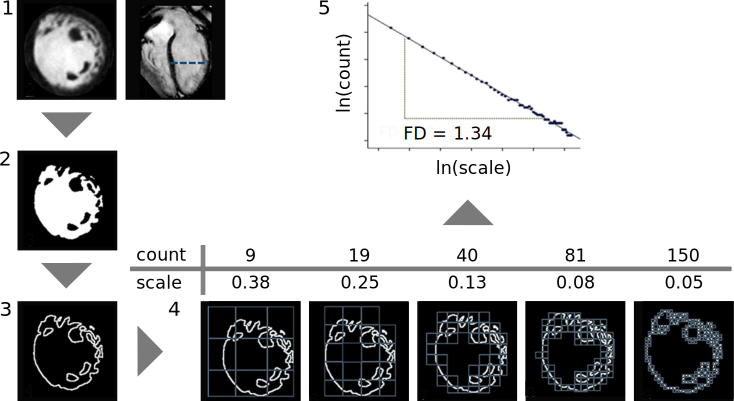
\includegraphics[trim = 0mm 0mm 0mm 0mm, clip, width=\textwidth]{Chapter6/Figures/FD_scheme.pdf}
	\caption[\textbf{FD phenotyping scheme. }]{\textbf{FD phenotyping scheme. }FD is determined for each of the LVSA slices derived from standard 2D CMR images. 1. An example LVSA slice is depicted on the left, its location in the heart is indicated by the dashed line of the heart image on the right. 2. The image is binarised into blood pool (white) and other structures (black). 3. The border between the white and the black background is the endocardial wall, which can be extracted via edge detection. 4. A standard box-counting method is applied to the image of the extracted border, where grids of known spacing (scale) are placed on top of the image and boxes containing at least one pixel of endocardial borders are counted. 5. The slope of the regression of the ln-transformed scale versus the ln-transformed count is the FD. Adapted from \citep{Captur2013}.} 
	 	\label{fig:scheme-fd}
\end{figure}

\section{The complexity of trabeculation shows a consistent base to apex pattern}
For \num{1192} out of the \num{1207} genotyped samples, FD measurements could successfully be computed at each slice. Their distribution from base to apex is depicted in \cref{fig:perslice-fd}. Both at the tip of the apex and the end of the basal zone, FD is generally lowest and increases towards the mid-section of the heart. Similar results have been observed by \citep{Kawel2012} and \citep{Captur2014}. The latter have shown that most variation between healthy and diseased individuals exists in FD measurements derived from the apical slices of the heart ( \cref{fig:perslice-fd}\subfig{A}) and used the maximal FD value observed in these slices as their final phenotype. I followed the strategy of dividing the measurements into apical and basal (\cref{fig:perslice-fd}\subfig{B}) and used the maximum FD observed in each group as final phenotypes. For individuals with uneven numbers of slices, the center slice was not considered for the computation of the maximum values.
\\
\begin{figure}[hbtp]
	\centering
	\includegraphics[trim = 0mm 0mm 0mm 0mm, clip, width=\textwidth]{Chapter6/Figures/FDalongHeart.pdf}
	\caption[\textbf{FD measurements from base to apex. }]{\textbf{FD measurements from base to apex. } A. Location of the 2D CMR slices and their classification into apical and basal. B. FD measurements for all samples were interpolated via a cubic spline function to the maximum number of \num{10} slices for easier visualisation. Subsequent analyses were done based on the original, non-interpolated FD measurements.} 
	 	\label{fig:perslice-fd}
\end{figure}

\section{Relationship between trabeculation phenotypes and covariates}
\begin{figure}[hbtp]
	\centering
	\includegraphics[trim = 0mm 0mm 0mm 0mm, clip, width=\textwidth]{Chapter6/Figures/pairs_fdcovariates.pdf}
	\caption[\textbf{Relationship between FD measures and covariates. }]{\textbf{Relationship between FD measures and covariates. }Continuous variables: the univariate-distribution of each variable is depicted on the diagonal. The upper triangular matrix shows the bi-variate distribution while the lower triangular matrix shows the regression line of their linear fit. Categorical variables (sex): Distribution (first row) and counts (first column) are depicted. } 
	 	\label{fig:covariates-FD}
\end{figure}

I analysed the distribution of the \num{2} FD measurements  \(\text{FD}_\text{max}^\text{basal}\) and \(\text{FD}_\text{max}^\text{apical}\)in relation to biological and cardiac covariates. \Cref{fig:covariates-FD} shows the distribution of FD measurements and covariates, both as their respective univariate distribution (diagonal) and their dependent distributions. Both FD measurements show significant correlation with age, weight and left ventricular mass.   \(\text{FD}_\text{max}^\text{basal}\) is additionally significantly associated with height, while  \(\text{FD}_\text{max}^\text{apical}\) also shows significant correlation with sex (\cref{tab:covariates-FD}). The association of LVM and \(\text{FD}_\text{max}^\text{apical}\)  confirms the findings of the study by Captur and colleagues \citep{Captur2014}, who found increased FD measures for individuals with increased LVM. However, the causality of the relationship has not been determined yet. All significantly associated covariates except for LVM, as the causal relationship to FD measurements is unclear, were used as covariates in the genome-wide association study. 

% Table generated by Excel2LaTeX from sheet 'FDCovariates'
\begin{table}[htbp]
  \centering
  \caption[\textbf{Association of \(\text{FD}_\text{max}^\text{basal}\) and \(\text{FD}_\text{max}^\text{apical}\) with covariates. }]{\textbf{Association of \(\text{FD}_\text{max}^\text{basal}\) and \(\text{FD}_\text{max}^\text{apical}\) with covariates. } Association was determined based on a simple linear model for each FD measurement with all covariates as explanatory variables without interaction effects.}
    \begin{tabular}{lll}
    \toprule
          &  \(\text{FD}_\text{max}^\text{basal}\) & \(\text{FD}_\text{max}^\text{apical}\) \\
    \midrule
    Sex   & \num{5.47E-01} & \num{4.96E-03} \\
    Age   & \num{3.04E-08} & \num{2.87E-04} \\
    Height & \num{4.33E-02} & \num{4.43E-01} \\
    Weight & \num{1.25E-04} & \num{4.55E-05} \\
    LVM   & \num{1.21E-12} & \num{2.62E-03} \\
    Slices & \num{8.02E-01} & \num{3.89E-01} \\
    \bottomrule
    \end{tabular}%
  \label{tab:covariates-FD}%
  \vspace{-2mm}
\end{table}%
\section{Left ventricular trabeculation is associated with two genomic loci}
The extraction of \gls{fd} measurements from the 2D cardiac magnetic resonance images yields quantitative phenotypes capturing the complexity of trabeculation in the left ventricle. I used the two summary measures \(\text{FD}_\text{max}^\text{basal}\) and \(\text{FD}_\text{max}^\text{apical}\) described above as the response variables in a \gls{mtgwas} with the genetic marker and sex, age, height and weight as covariates. Since the dataset contained related individuals, I extended to model used in \cref{section:GWAS-3Dheart} to a \gls{lmm} by including an additional random genetic effect based on the \gls{rrm} of the samples. The \gls{rrm} was estimated from the samples' genotypes as described in \cref{subsubsection:grm}. The manhattan and qq-plots for the joint analysis of \(\text{FD}_\text{max}^\text{basal}\) and \(\text{FD}_\text{max}^\text{apical}\) are depicted in \cref{fig:manhattan-FD} and \cref{fig:qq-FD}, showing two loci that reach genome-wide significance. As a comparison, \gls{stgwas} of  \(\text{FD}_\text{max}^\text{basal}\) and \(\text{FD}_\text{max}^\text{apical}\) only discovered the association on chromosome 2 (with response variable \(\text{FD}_\text{max}^\text{apical}\); \cref{fig:manhattan-FD-single}), demonstrating the power of the multi-trait approach.
%
\begin{figure}[hbtp]
	\centering
	\includegraphics[trim = 0mm 0mm 0mm 0mm, clip, width=\textwidth]{Chapter6/Figures/lm_mt_pcs_manhattanplot.png}
	\caption[\textbf{Manhattan plot of multi-trait GWAS on left ventricular trabeculation. }]{\textbf{Manhattan plot of multi-trait GWAS on left ventricular trabeculation. } The maximal apical and basal \gls{fd} were modelled jointly in an any effect \gls{mtgwas}. The p-values of all genome-wide \glspl{snp} are depicted. The horizontal grey line is drawn at the level of genome-wide significance: \(p = 5 \times 10^{-8}\).} 
	 	\label{fig:manhattan-FD}
\end{figure}
%
\begin{figure}[hbtp]
	\centering
	\includegraphics[trim = 0mm 0mm 0mm 0mm, clip, width=0.6\textwidth]{Chapter6/Figures/lm_mt_pcs_qqplot.png}
	\caption[\textbf{Quantile-quantile plot of multi-trait GWAS on left ventricular trabeculation .}]{\textbf{Quantile-quantile plot of multi-trait GWAS on left ventricular trabeculation.} The observed genome-wide p-values of the multi-trait \gls{fd} \gls{gwas} are plotted against equally spaced values in \([0,1]\) of the same sample size (expected p-values). The diagonal line starts at the origin and has slope one.} 
	 	\label{fig:qq-FD}
\end{figure}
%
\noindent A summary of the two loci that reach genome-wide significance is shown in \cref{tab:sig-FD} and \cref{fig:locuszoom-fd}. The locus on chromosome~2 lies within an intron of a long intergenic noncoding RNAs (lincRNA) of unknown function (\cref{fig:locuszoom-fd}, upper panel). The second associated locus is positioned in intron \num{24} of the \textit{ADAMTSL1} gene (\cref{fig:locuszoom-fd}, lower panel). \textit{ADAMTSL1} is also known as \textit{Punctin} and two of its intronic and intergenic variants  (rs7869627: intron \num{17}; rs1411242: intergenic between \textit{SH3GL2} and \textit{ADAMTSL1}) have been found associated with blood pressure phenotypes \citep{Sabatti2009}. rs7855681 is in weak \gls{ld} with rs7869627 ( \(r^2=0.119\)). 

% Table generated by Excel2LaTeX from sheet 'AssociationFD'
\begin{table}[htbp]
  \centering
  \caption[\textbf{SNPs with strongest association in left ventricular trabeculation GWAS. }]{\textbf{SNPs with strongest association in left ventricular trabeculation GWAS. } For each locus, the p-values for \glspl{snp} in \gls{ld} with an \(r^2 > 0.8\) in a \num{50}kb window were compared and only the \gls{snp} with smallest p-value per locus listed below. M allele: major allele, m allele:  minor allele, MAF: minor allele frequency. }
    \begin{tabular}{lrllll}
    \toprule
    SNP   & \multicolumn{1}{l}{Chr} & Position & P-value & M/m allele & MAF \\
    \midrule
    rs7603133 & 2     & \num{3103708} & \num{3.23E-08} & A/G     & \num{0.09} \\
    rs7855681 & 9     & \num{18855498} & \num{3.46E-08} & A/C     & \num{0.32} \\
    \bottomrule
    \end{tabular}%
  \label{tab:sig-FD}%
\end{table}%
%
\begin{figure}[hbtp]
	\centering
	\includegraphics[trim = 0mm 0mm 0mm 0mm, clip, width=0.8\textwidth]{Chapter6/Figures/locuszoom.png}
	\caption[\textbf{Genomic context of loci associated loci with left ventricular trabeculation. }]{\textbf{Genomic context of loci associated loci with left ventricular trabeculation.  }The p-values and genomic location of the two loci reaching genome-wide significance are shown in relation to the p-values of surrounding genotypic markers. Markers are coloured by the level of \gls{ld} they share with the \gls{snp} of interest. For both loci, all \glspl{snp} that are associated were imputed. For the locus on chromosome~9 (lower panel), an additional \gls{snp} which was directly genotypes but has not passed the genome-wide significant level has been marked in red. Generated with LocusZoom \citep{Pruim2010}.}  
	 	\label{fig:locuszoom-fd}
\end{figure}
%
Punctin is a secreted glycoprotein that can be detected in contacts between cells and components of the extra-cellular matrix, but that has not been observed in cell-cell contacts \citep{Hirohata2002}. It is part of the ADAMTS-like protein family which lack the proteolytic activity of their name-lending metalloprotease protein family. While other proteins of the ADAMTS-like family have been shown to be associated with connective tissue disorders and affecting the formation of the extra-cellular matrix \citep{Ahram2009,Hubmacher2015}, the function of punctin remains unknown. However, progress has been made in understanding the regulation of its secretion through post-translational modification of its tryptophane \num{42} residue \citep{Wang2009}. A recently published study shows a strong systemic phenotype for the mutation of this tryptophane residue, inhibiting the secretion of the protein. However, no further advances in understanding the mechanisms or finding binding partners of ADAMTSL1 could be made \citep{Hendee2017}.

The locus on chromosome~1 (SNP: rs113719231 ) discovered in \cref{section:GWAS-3Dheart} is located near the \textit{PRDM16} gene which has been associated with \gls{lvnc} \citep{Arndt2013}. A linear model with the rs113719231 genotypes, sex, age, height and weight as explanatory variables and \(\text{FD}_\text{max}^\text{basal}\)/\(\text{FD}_\text{max}^\text{apical}\) as response variables did not show any association, even without the burden of the genome-wide significance threshold (\(p = 0.78\)/\(p = 0.77\)).

The clinical phenotype of left ventricular non-compaction has been found associated with a number of other cardiac and cardiovascular phenotypes such as conduction abnormalities \citep{Yousef2009}, arrhythmias \citep{Ritter1997,Oechslin2000,Yousef2009}, coronary artery disease \citep{Ritter1997,Junga1999,Jenni2002,Soler2002} and myocardial infarction \citep{Swinkels2007,Toufan2012,Guvens2012}. In addition, a study on population variation of left ventricular trabeculation found associations between the increase in left ventricular trabeculation and prevalence of hypertension, left ventricular mass and wall thickness \citep{Captur2015}. For the majority of these phenotypes, original \gls{gwas} and meta-analysis of \gls{gwas} have been conducted including atrial fibrillation \citep{Gudbjartsson2007,Christophersen2017}, atrioventricular conduction \citep{Denny2010}, coronary heart disease \citep{Schunkert2011,Lee2013a,Nikpay2015}, myocardial infarction \citep{Kathiresan2009,Hirokawa2015,Nikpay2015,Dehghan2016} and blood pressure phenotypes \citep{Ehret2011,Wain2011}. For studies where the summary statistics of the genome-wide associations were made publicly available (blood pressure phenotypes \citep{Ehret2011,Wain2011}, coronary artery disease \citep{Schunkert2011} and myocardial infarction \citep{Nikpay2015}), I collected the effect size estimate (continuous traits) and odds ratios (case-control setting) for the associated loci on chromosome 2 and 9. The \gls{snp} with the highest association on chromosome 9 (rs7855681) was contained in all available studies. For the locus on chromosome 2, the \gls{snp} with the highest association was not contained in any of the studies, however rs6758505 which is in strong \gls{ld} with the discovered \gls{snp} in Europeans (\(r^2=1\)) was found in one of the studies. \Cref{fig:consortia} depicts the effect size estimates and odds ratios for both \glspl{snp}  estimated for different blood pressure measurements, coronary artery disease and myocardial infarction. For all phenotypes, the confidence intervals of effect size/odds ratio estimates contain zero and one, respectively and thus show no effect of the \glspl{snp}  on these phenotypes. 
%
\begin{figure}[hbtp]
	\centering
	\includegraphics[trim = 0mm 0mm 0mm 0mm, clip, width=0.8\textwidth]{Chapter6/Figures/forestplotCardioConsortia.pdf}
	\caption[\textbf{Effect estimates of associated FD SNPs with other cardiovascular phenotypes. }]{\textbf{Effect estimates of associated FD SNPs with other cardiovascular phenotypes. }Effect size estimates and odds rations for the \glspl{snp} associated with \gls{fd} were derived from previous published studies on blood pressure (BP) phenotypes and risk for coronary artery diseases and myocardial infarction. The diamond indicates the effect estimates, the error bars their confidence interval. The size of the diamond represents the sample size of the study and is normalised to the largest study size (pulse pressure: \(N=\)\num{71663}). All studies were conducted as meta-analyses in the scope of large consortia (faceting labels). The dashed vertical line indicates the value of no effect. }
%For the locus on chromsome 2, a SNP (rs6758505) in perfect lD with the discovered SNP (rs7603133) was contained in the analysis and its values are depicted (). For the locus on chromosome 9 the original SNP was contained in the studies. }  
	 	\label{fig:consortia}
\end{figure}
%
A database search of the \gls{gwas} catalogue \citep{MacArthur2017} for associated \glspl{snp} and \glspl{snp} in \gls{ld} (based on entries in the \gls{gwas} catalogue, 0.7.08.2018) and the Global Biobank engine \citep{GBE2017} did not yield associations with any other phenotype. 

\section{Summary}
In this chapter, I used phenotypes derived from a guided feature extraction method to map naturally occurring genetic variation in healthy individuals to a clinically relevant phenotype. The association of the \gls{fd} phenotypes as a quantification of left ventricular trabeculation detected two loci that are linked on a genome-wide significant level. Both loci lie in intronic regions and have no direct protein-coding consequences. Loci in proximity to the association detected within the ADAMTSL1 gene have been implicated in cardiac phenotypes such a blood pressure. However, the absence of any effect for this locus in well-powered published \gls{gwas} of blood pressure phenotypes points towards a blood pressure-independent effect on left ventricular trabeculation.

For quantitative, continuous phenotypes and additive genotype effects, understanding naturally occurring variation can give insights into the genetic architecture of the traits and might help to understand more extreme disease phenotypes. In order to extend this study and confirm results in a larger cohort, we applied for access to the UK Biobank a `large, population-based prospective study, established to allow detailed investigations of the genetic and non-genetic determinants of the diseases of middle and old age' \citep{Sudlow2015}. Within this project, \num{500000} individuals have been genotyped and phenotyped for wide array of traits, including 2D cardiac magnetic resonance imaging scans on an expected \num{100000} individuals. In contrast to the 3D heart phenotypes investigated in \cref{chapter:GWAS-3Dheart}, the \gls{fd} phenotypes can be automatically extracted from these images. Upon access to the data,  phenotype extraction and a \gls{mtgwas} with the same model and parameters as described in this chapter will be conducted. 

In addition to this replication study, investigating the genetic variation driving the healthy phenotype differences in individuals of different ethnicities \citep{Kawel2012,Captur2014} will be of great interest. While the cohort in this study only contained a minority of non-European samples, a more diverse cohort structure might be observed in the UK Biobank cohort, enabling this analysis. 


\section{LiMMBo for multi-trait GWAS and beyond}
\label{section:conclusion-limmbo}
In this chapter, I introduced \gls{limmbo}, a new method for the multivariate analysis of large trait numbers, which uses a bootstrap method to estimate complex trait covariance matrices. The main benefit of \gls{limmbo} is that it scales to \num{100}s of phenotypes, both because of its inherent sub-sampling method and that the most computationally intense part of the method can be parallelised. To take advantage of the parallelisation, I implemented an optional automatic detection for multiple cores which allows for easy realisation of this process via the \textit{Parallel Python Software} \citep{PPSoftware}. In practice, this means that trait sizes up to 30 or 40 can be in hours, rather than taking several days as for standard \gls{reml}-based methods. Most notably, complex datasets of \num{100}s of traits, which is out of scope for the \gls{reml} approaches, are feasible when using \gls{limmbo}. I showed that the covariance matrices estimated via \gls{limmbo} are as good an estimator of the real covariance matrices as the ones of the validated \gls{reml} approach. Consequently, these covariance matrices produce well calibrated null models when used in \gls{lmm} for \gls{gwas}, showing the validity of the approach. To show the advance of \gls{limmbo}, I demonstrated the power gain for multi-trait \gls{gwas} of high-dimensional phenotypes with \gls{limmbo} over standard single-trait models across a wide range of phenotype architectures. I made \gls{limmbo} accessible as an open source, python module at \url{https://github.com/HannahVMeyer/LiMMBo/tree/master/limmbo}. \gls{limmbo} is compatible with the LIMIX package for linear mixed models \citep{Lippert2014}.  

The bootstrapping has proven powerful to reduce the computational complexity for estimating the covariance parameters and made the analysis of complex datasets with high trait numbers possible. However, so far, I only examined the complexity and calibration dependent on the size of the overall phenotype set \(P\). Of additional interest would be understanding the (co-)dependence of the bootstrap size \(s\),  the number of bootstraps \(b\) and the  co-sampling of traits \(c\). Based on already simulated datasets, a systematic comparison of the run times, covariance estimates and calibration of different combinations of \(s\) and \(b\) could be conducted. For each of these combinations, different thresholds for \(c\) could be examined.

Much of the attraction of linear mixed models in genetics has been their ability to model complex genetic relatedness. As described by \citep{Kang2010} and demonstrated in this chapter, simple linear models are not suitable for analysing phenotypes with complex underlying genetic relatedness, whereas linear mixed models with the covariance matrices estimated by \gls{limmbo} are appropriate and possible up to \num{100}s of traits. Complex relatedness in populations is wide-spread in plant and animal breeding \citep{Bolormaa2014,Yang2014}, and increasingly common in human bottleneck populations \citep{Tachmazidou2013}. Furthermore, as the population numbers increase in human genetics, complex cryptic relationship structures are more prevalent \citep{Reich2001}, meaning that methods such as \gls{limmbo} will be more applicable in the future in human genetics. 

Trait-by-trait covariance matrices are useful for a variety of high dimensional big data problems across genomics, from statistical genetics to single cell analysis. The ability to accurately estimate large trait-by-trait covariance matrices using this bootstrap method may be applicable to more domains than \gls{gwas}, e.g. many gene expression studies use covariance matrices. Previous work from \citet{Schaefer2005} showed the large gene dimensions coupled with small(er) sample sets means that empirical covariance matrices could not be accurately estimated; other investigators \citep{Ledoit2004,Furrer2007,Bickel2008} used shrinkage methods to create valid covariance matrices. The work from \citet{Teng2009} uses subsampling but with strong shrinkage priors to generate the final covariance matrix. By fitting the average to closest true covariance, \gls{limmbo} ensures positive-semidefiniteness of the covariance while avoiding ill-conditioned matrices, which usually introduces large biases in the final use of these models. Thus, covariance estimation based on the method implemented in \gls{limmbo} might be applicable and useful in other areas of quantitative genetics.  

The ability to generate large cohorts of well phenotyped and genotyped individuals has forced the development of many new methods in statistical genetics. With the advent of genotyped human cohorts up to \num{500000} individuals with over \num{2000} different traits \citep{Sudlow2015}, and plant phenotyping routinely in the \num{1000}s of individuals from structured crosses with \num{100}s of (image-based) phenotypes \citep{Atwell2010,Yang2014}, new informative and scaleable methods are needed. \gls{limmbo} extends the reach of linear mixed models into this new regime, allowing for new complex genetic associations to be made.


\beginsupplement
\section{Quality control: genotyping}

\begin{figure}[hbtp]
	\centering
	\includegraphics[trim = 0mm 0mm 0mm 20mm, clip, width=0.8\textwidth]{Figures/Venn_genotyping_batches.png}
	\caption{\textbf{.} .}
 	\label{fig:probeoverlap}
\end{figure}

\begin{figure}[hbtp]
	\centering
	\includegraphics[trim = 0mm 0mm 0mm 20mm, clip, width=0.8\textwidth]{Figures/SampleQC.pdf}
	\caption{\textbf{.} .}
 	\label{fig:sampleQC}
\end{figure}

\begin{figure}[hbtp]
	\centering
	\includegraphics[trim = 0mm 0mm 0mm 20mm, clip, width=0.8\textwidth]{Figures/SNPQC.pdf}
	\caption{\textbf{.} .}
 	\label{fig:SNPQC}
\end{figure}

\begin{figure}[hbtp]
	\centering
	\includegraphics[trim = 0mm 0mm 0mm 20mm, clip, width=0.8\textwidth]{Figures/kinshipQC.pdf}
	\caption{\textbf{.} .}
 	\label{fig:kinshipQC}
\end{figure}

\section{Quality control: imputation}

\begin{figure}[hbtp]
	\centering
	\includegraphics[trim = 0mm 0mm 0mm 20mm, clip, width=0.8\textwidth]{Figures/perBatchSNPsperChr.pdf}
	\caption{\textbf{.} .}
 	\label{fig:imputeQC}
\end{figure}


\titleformat*{\chapter}{\normalfont}
\printbibliography[heading=bibintoc]


\end{document}


